\documentclass[10pt]{mypackage}

% sans serif font:
%\usepackage{cmbright}
%\usepackage{sfmath}
%\usepackage{bbold} %better blackboard bold

%serif font + different blackboard bold for serif font
\usepackage{newpxtext,eulerpx,eucal}
\renewcommand*{\mathbb}[1]{\varmathbb{#1}}

%\usepackage{mathrsfs}
%\usetikzlibrary{arrows}
\pagestyle{fancy}
\fancyhf{}
\rhead{Avinash Iyer}
\lhead{Ordinary Differential Equations: Class Notes}

\setcounter{secnumdepth}{0}

\begin{document}
\tableofcontents
\section{First-Order Differential Equations}%
\subsection{Introduction to First-Order Differential Equations}%
  Recall that for $y = f(x)$, $x$ is the independent variable and $y$ is the dependent variable.
  \begin{definition}[Differential Equation]
  A differential equation is an equation which contains derivatives of a dependent variable with respect to one or more independent variables.
  \end{definition}
  \begin{example}[A Basic Differential Equation]
    \begin{align*}
      \frac{dy}{dx} - 5y - 1 &= 0
    \end{align*}
  \end{example}
  We can classify differential equations by
  \begin{itemize}
    \item type;
    \item order;
    \item linearity.
  \end{itemize}
  \begin{definition}[Classification by Type]
  There are two types of differential equations:
  \begin{itemize}
    \item ordinary differential equations (ODEs);
    \item partial differential equations (PDEs).
  \end{itemize}
  ODEs are characterized by derivatives of the dependent variable with respect to one independent variable. PDEs are characterized by derivatives of the dependent variable with respect to multiple independent variables.
  \end{definition}
  \begin{example}[ODEs and PDEs]\hfill
    \begin{enumerate}[(1)]
      \item An ODE:
        \begin{align*}
          \frac{d^2y}{dx^2} - 2\frac{dy}{dx} + 6y &= 0
        \end{align*}
      \item A PDE:
        \begin{align*}
          \pd{^2u}{x^2} + \pd{^2u}{y^2} &= 0
        \end{align*}
    \end{enumerate}
  \end{example}
  \begin{definition}[Classificiation by Order]
    The order of the highest derivative in a differential equation is the order of the differential equation.
  \end{definition}
  \begin{example}[Differential Equations of Varying Orders]\hfill
    \begin{enumerate}[(1)]
      \item 
        \begin{align*}
          \diff{^2y}{x^2} + 5\left(\frac{dy}{dx}\right) - 4y &= x \tag*{order 2}
        \end{align*}
      \item 
        \begin{align*}
          2\frac{dy}{dx} + y &= 0\tag*{order 1}
        \end{align*}
      \item 
        \begin{align*}
          \sin(x)y''' - \left(\cos x\right)y' &= 2\tag*{order 3}
        \end{align*}
    \end{enumerate}
  \end{example}
  In general, we write a differential equation of order $n$ in the form
  \begin{align*}
    \underbrace{F\left(x,y,\frac{dy}{dx},\frac{d^2y}{dx^2},\dots,\frac{d^ny}{dx^n}\right)}_{\text{$n+2$ variables}} = 0.
  \end{align*}
  \begin{example}
    Suppose we have the differential equation
    \begin{align*}
      \frac{d^3y}{dx^3} + y^2 &= x.
    \end{align*}
    Then, we rewrite as
    \begin{align*}
      \underbrace{\frac{d^3y}{dx^3} + y^2 - x}_{F\left(x,y,\frac{dx}{dy},\frac{d^2x}{dy^2},\frac{d^3x}{dy^3}\right)} &= 0.
    \end{align*}
    Alternatively, we can write as
    \begin{align*}
      \frac{d^3y}{dx^3} &= \underbrace{x - y^2}_{f(x,y)}.
    \end{align*}
  \end{example}
  \begin{definition}[Classification by Linearity]
    We much prefer to analyze linear differential equations over nonlinear differential equations.\newline

    A differential equation is linear if it has the following form:
    \begin{align*}
      a_n(x)\frac{d^ny}{dx^n} + a_{n-1}(x)\frac{d^{n-1}y}{dx^{n-1}} + \cdots + a_{1}(x)\frac{dy}{dx} + a_0(x)y &= g(x).
    \end{align*}
    \begin{enumerate}[(1)]
      \item The power of each term involving $y$ and all its derivatives is one.
      \item All coefficients are exclusively functions of $x$.
    \end{enumerate}
    A differential equation that is not linear is called nonlinear.
  \end{definition}
  \begin{example}[Linear Differential Equations (or lack thereof)]\hfill
    \begin{enumerate}[(1)]
      \item 
        \begin{align*}
          x^3\frac{d^3y}{dx^3} - x^2\frac{d^2y}{dx^2} + 3x\frac{dy}{dx} + 5y &= e^x \tag*{Linear}
        \end{align*}
      \item 
        \begin{align*}
          yy'' - 2y' &= x\tag*{Nonlinear}
        \end{align*}
      \item 
        \begin{align*}
          \frac{d^3y}{dx^3} + y^2 &= 0 \tag*{Nonlinear}
        \end{align*}
    \end{enumerate}
  \end{example}
  \begin{definition}[Autonomous Differential Equations]
    An autonomous (first-order) differential equation is a differential equation in the following form:
    \begin{align*}
      \frac{dy}{dx} &= f(y).
    \end{align*}
  \end{definition}
  \begin{definition}[Solution to an ODE]
    Consider the general ODE
    \begin{align*}
      F\left(x,y,\frac{dy}{dx},\frac{d^2y}{dx^2},\dots,\frac{d^ny}{dx^n}\right) &= 0.\tag*{(\textasteriskcentered)}
    \end{align*}
    A solution of (\textasteriskcentered) is a function $y = f(x)$ that satisfies the ODE; that is,
    \begin{align*}
      F\left(x,f(x),f'(x),f''(x),\dots,f^{(n)}(x)\right) &= 0
    \end{align*}
    for every $x$ in the domain of $f(x)$.\newline

    Notice that $f$ is an element of a family of functions that satisfy the differential equation.
  \end{definition}
  \begin{example}[Verifying a Solution]
    We wish to show that $y = xe^{x}$ is a solution to
    \begin{align*}
      y'' - 2y' + y &= 0
    \end{align*}
    on $(-\infty,\infty)$.\newline

    In order to do this, we plug the proposed solution into the ODE:
    \begin{align*}
      y'' - 2y' + y &= \frac{d^2}{dx^2}\left(xe^{x}\right) - 2\frac{d}{dx}\left(xe^x\right) + xe^x\\
                    &= \left(xe^x + 2e^x\right) - 2\left(xe^x + e^x\right) + xe^x\\
                    &= 0.
    \end{align*}
  \end{example}
  \begin{definition}[Equilibrium Solution]
    An equilibrium solution of a differential equation is a \textit{constant function} that satisfies the differential equation.
  \end{definition}
  \begin{example}
    We want to find equilibrium solutions for the following equations:
    \begin{enumerate}[(1)]
      \item $\frac{dy}{dt} = 2-y$
      \item $\frac{dy}{dt} = y^2 - 3y - 4$.
    \end{enumerate}
    In order to find equilibrium solutions, we know that $\frac{dy}{dt} = 0$. Thus, the equilibrium solutions are, respectively,
    \begin{enumerate}[(1)]
      \item $y(t) = 2$
      \item $y(t) = -1$ or $y(t) = 4$.
    \end{enumerate}
  \end{example}
  For first-order ODEs of the form
  \begin{align*}
    \frac{dy}{dt} = f(t,y),
  \end{align*}
  equilibrium solutions are found by taking $\frac{dy}{dt} = 0$, and solving for $y$.
  \subsection{Modeling with Differential Equations}%
  \begin{definition}[Initial Value Problem]
  An initial value problem is a problem with a given ODE and an initial condition.
  \end{definition}
  \begin{example}[Initial Value Problems]\hfill
    \begin{enumerate}[(1)]
      \item We want to find
    \begin{align*}
      \frac{dy}{dx} &= f\left(x,y\right)
    \end{align*}
    such that $y\left(x_0\right) = y_0$.
    \item
      \begin{align*}
        \frac{d^2y}{dx^2} &= f\left(x,y,\frac{dy}{dx}\right)
      \end{align*}
      must satisfy $y\left(x_0\right) = y_0$, $y'\left(x_0\right) = y_1$.
    \end{enumerate}
  \end{example}
  Modeling primarily occurs via the following feedback loop:
  \begin{itemize}
    \item real-world problem;
    \item mathematical model;
    \item solution;
    \item result/prediction.
  \end{itemize}
  As predictions from the model begin to stray from real-world observations, we update the model to reflect these new observations.
  \begin{example}[Vertical Motion]
    Consider someone who throws a rock off a building.\newline

    We let $y(t)$ denote the height of the ball at time $t$, with $y_0$ denoting initial height. The acceleration due to gravity is equal to $a(t) = v'(t) = y''(t) = g$.\newline

    Our ODE is
    \begin{align*}
      y''(t) &= -g \tag*{for $0 \leq t \leq T$.}
    \end{align*}
    We require some initial conditions:
    \begin{itemize}
      \item $y(0) = y_0$ (initial position);
      \item $y'(0) = v_0$ (initial velocity).
    \end{itemize}
    Thus, we have created our second-order initial value problem.\newline

    To solve this second-order initial value problem analytically, we start with
    \begin{align*}
      y'' &= -g.
    \end{align*}
    Taking our first integral with respect to $t$, we have
    \begin{align*}
      y' &= -gt + c_1.
    \end{align*}
    Now, taking our second integral, 
    \begin{align*}
      y(t) &= -\frac{1}{2}gt^2 + c_1 t + c_2.
    \end{align*}
    This version of $y(t)$ is the general solution.\newline

    Applying our initial condition on $y'(t)$, we have $y'(0) = c_1$, meaning $c_1 = v_0$, and applying the initial condition to $y(t)$, we have $y(0) = c_2$, meaning $c_2 = y_0$.\newline

    Thus, the solution to this initial value problem is
    \begin{align*}
      y(t) &= -\frac{1}{2}gt^2 + v_0 t + y_0.
    \end{align*}
  \end{example}
  \begin{example}[Population Growth, Exponential and Logistic]
    Let $P(t)$ be the population of living fish in a lake at time $t$.\newline

    We know that the rate of growth in population is proportional to the population. In other words,
    \begin{align*}
      \frac{dP}{dt} &= kP(t)
    \end{align*}
    for some constant $k > 0$.\newline

    We can also include an initial condition, $P(0) = P_0$.\newline

    We can see (relatively easily) that
    \begin{align*}
      P(t) &= P_0e^{kt}.
    \end{align*}
    However, this is not particularly realistic; there is no theoretical upper bound on the model, even though in real life, ecosystems tend to have carrying capacities.\newline

    The logistic population model with growth rate $k$ and carrying capacity $N$ is is
    \begin{align*}
      \frac{dP}{dt} &= kP\left(1 - \frac{P}{N}\right).
    \end{align*}
    We can analyze this equation qualitatively first (before finding an analytical solution).
    \begin{itemize}
      \item If $P > N$, we can see that $\frac{dP}{dt} < 0$, which is expected since, if population is greater than carrying capacity, we expect population to approach carrying capacity.
      \item If $P < N$ (assuming $P$ is positive), we see that $\frac{dP}{dt} > 0$, meaning population increases as it approaches carrying capacity. In particular, as population increases, the growth rate decreases.
      \item The equilibrium solutions occur at $P = 0$ or $P = N$.
    \end{itemize}
    \begin{center}
      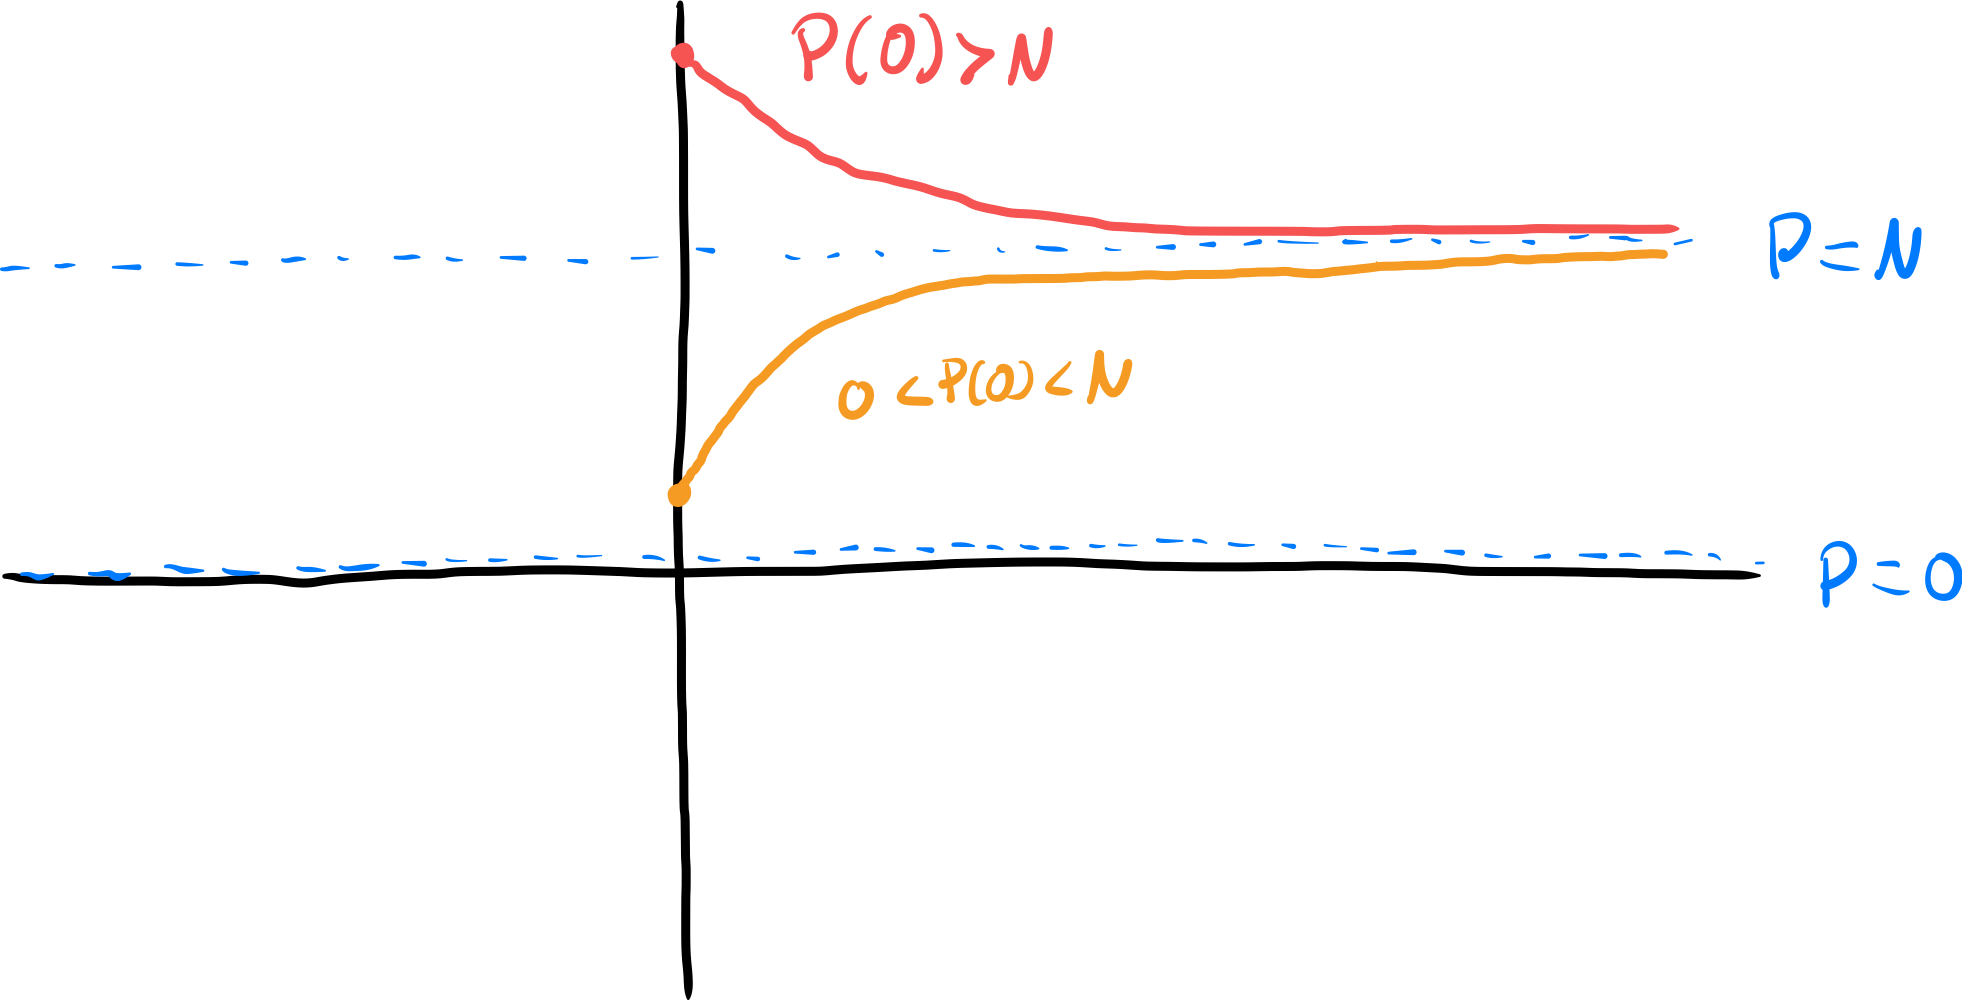
\includegraphics[width=10cm]{images/logistic_map.png}
    \end{center}
  \end{example}
\subsection{Separable First-Order Differential Equations}%
Consider the first-order differential equation
\begin{align*}
  \frac{dy}{dt} &= f(t,y).
\end{align*}
\begin{definition}[Separable Differential Equation]
  A differential equation of the form
  \begin{align*}
    \frac{dy}{dt} &= g(t)h(y)
  \end{align*}
  is called separable.
\end{definition}
\begin{note}
\begin{align*}
  f(t,y) = g(t)h(y).
\end{align*}
\end{note}
\begin{example}\hfill
  \begin{enumerate}[(1)]
    \item We can see that $\frac{dP}{dt} = kP$ is separable; $g(t) = k$, $h(y) = P$.
    \item We can see that $\frac{dy}{dt} = -\frac{t}{y}$ is also separable; $g(t) = -t$, $h(y) = \frac{1}{y}$.
    \item We can see that $\frac{dy}{dt} = y + t$ is not separable.
  \end{enumerate}
\end{example}
\begin{method}[Separation of Variables]
  We want to solve $\frac{dy}{dt} = g(t)h(y)$.
  \begin{enumerate}[(1)]
    \item We take $\frac{dy}{h(y)} = g(t)\:dt$ by multiplying $dt$ on both sides and dividing by $h(y)$.
    \item Integrate both sides with respect to their corresponding variable, yielding
      \begin{align*}
        \int_{}^{} \frac{1}{h(y)}\:dy &= \int_{}^{} g(t)\:dt.
      \end{align*}
    \item We get
      \begin{align*}
        H(y) &= G(t) + C,
      \end{align*}
      where $H(y)$ and $G(t)$ are antiderivatives of $\frac{1}{h(y)}$ and $g(t)$ respectively.
  \end{enumerate}
\end{method}
\begin{example}[Solving the Exponential Population Growth Model by Separation of Variables]
  Let $\frac{dP}{dt} = kP$, $P(0) = P_0$.
  \begin{align*}
    \frac{dP}{dt} &= kP\\
    \frac{dP}{P} &= k\:dt\\
    \int_{}^{} \frac{1}{P}\:dP &= \int_{}^{} k\:dt\\
    \ln|P| &= kt + C\\
    |P| &= e^{kt + C}\\
      &= e^{kt}e^{C}\\
    P &= \left(\pm e^{C}\right)e^{kt}\\
      &= Ae^{kt}.
  \end{align*}
  Our solution is now of the form $P(t) = Ae^{kt}$ (where $A = \pm e^{C}$). This is not the general solution, though, since it lacks our equilibrium solution of $P = 0$. Thus, the general solution is
  \begin{align*}
    \begin{cases}
      P(t) = Ae^{kt}\\
      P(t) = 0
    \end{cases}
  \end{align*}
  With the initial condition of $P(0) = P_0$, we have
  \begin{align*}
    P_0 = P(0)
         &= Ae^{k\cdot 0}\\
         &= A.
  \end{align*}
  Thus, the particular solution to our initial value problem is $P(t) = P_0e^{kt}$.
\end{example}
\begin{example}[Solving a Sample Differential Equation by Separation of Variables]
  Let $\frac{dy}{dt} = y^2 - 4$. Note that, even though this is not a linear equation, this is a separable equation. We start with the equilibrium solutions, which are at $y(t) = 2$ and $y(t) = -2$.\newline

  If $y\neq \pm 2$, we have
  \begin{align*}
    \frac{dy}{dt} &= y^2 - 4\\
    \frac{1}{y^2 - 4}\:dy &= dt\\
    \int_{}^{} \frac{1}{4(y-2)} - \frac{1}{4(y+2)}\:dy &= \int_{}^{} \:dt\\
    \frac{1}{4}\left(\ln\left|\frac{y-2}{y+2}\right|\right) &= t + C_1\\
    \ln \left\vert \frac{y-2}{y+2} \right\vert &= 4t + C_2\\
    \left\vert \frac{y-2}{y+2} \right\vert &= e^{C_2}e^{4t}\\
                                           &= C_3e^{4t}\\
    \frac{y-2}{y+2} &=  \pm C_3 e^{4t}\\
                    &= C e^{4t}\\
    y &= 2 + y Ce^{4t} + 2Ce^{4t}\\
    y &= \frac{2\left(1 + Ce^{4t}\right)}{1-Ce^{4t}}.
  \end{align*}
  Thus, our general solution is
  \begin{align*}
    \begin{cases}
     y(t) = \frac{2\left(1 + Ce^{4t}\right)}{1-Ce^{4t}} \\
     y(t) = 2\\
     y(t) = -2
    \end{cases}
  \end{align*}
\end{example}
\begin{example}[Solving the Logistic Population Growth Model]
  Let $\frac{dP}{dt} = kP\left(1-\frac{P}{N}\right)$. Our equilibrium solutions are at $P(t)=0$ and $P(t)=N$. For non-equilibrium solutions, we have
  \begin{align*}
    \frac{dP}{dt} &= kP\left(1-\frac{P}{N}\right)\\
    \frac{1}{P\left(1-\frac{P}{N}\right)}\: dP &= k\:dt\\
    \int_{}^{} \frac{1}{P\left(1-\frac{P}{N}\right)}\:dP &= \int_{}^{} k\:dt\\
    \int_{}^{} \frac{-N}{P\left(P-N\right)}\:dP &= kt + C_1\\
    \int_{}^{} \frac{1}{P} - \frac{1}{P-N}\:dP &= kt + C_1\\
    \ln \left\vert P \right\vert - \ln \left\vert P-N \right\vert &= kt + C_1\\
    \ln \left\vert \frac{P}{P-N} \right\vert &= kt + C_1\\
    \left\vert \frac{P}{P-N} \right\vert &= e^{C_1}e^{kt}\\
    \frac{P}{P-N} &= \pm e^{C_1}e^{kt}\\
                  &= Ce^{kt}\\
    P\left(1-Ce^{kt}\right) &= -NCe^{kt}\\
    P &= N\frac{Ce^{kt}}{Ce^{kt} - 1}.
  \end{align*}
  Therefore, our general solution is
  \begin{align*}
    \begin{cases}
      P(t) = N\frac{Ce^{kt}}{Ce^{kt} - 1}\\
      P(t) = 0\\
      P(t) = N
    \end{cases}.
  \end{align*}
\end{example}
\begin{example}[A Non-Separable Linear Differential Equation]
  Consider the linear differential equation
  \begin{align*}
    \frac{dy}{dt} + a(t) y &= b(t).
  \end{align*}
  Notice that
  \begin{align*}
    \frac{dy}{dt} &= -a(t)y + b(t),
  \end{align*}
  which is not able to be separated.\newline

  In order to solve such an equation, we will need to use an integrating factor.
\end{example}
\subsection{Slope Fields}%
\begin{definition}
  A slope field is a set of short line segments that indicate slope $\frac{dy}{dx}$ at a set of points $(x,y)$ in the $x,y$-plane.\newline

  It is a graphical method of displaying the general slope and behavior of functions that satisfy $\frac{dy}{dx} = f(x,y)$.
\end{definition}
\begin{example}
  Consider $\frac{dy}{dx} = 1-y$. We can select some samples of slopes as follows:
  \begin{center}
    \begin{tabular}{c|c}
      Point & $\frac{dy}{dx}$\\
      \hline
      $(0,0)$ & $1$\\
      $(1,0)$ & $1$\\
      $(0,1)$ & $0$\\
      $(0,2)$ & $-1$
    \end{tabular}
  \end{center}
  Thus, we can draw the slope field:
  \begin{center}
    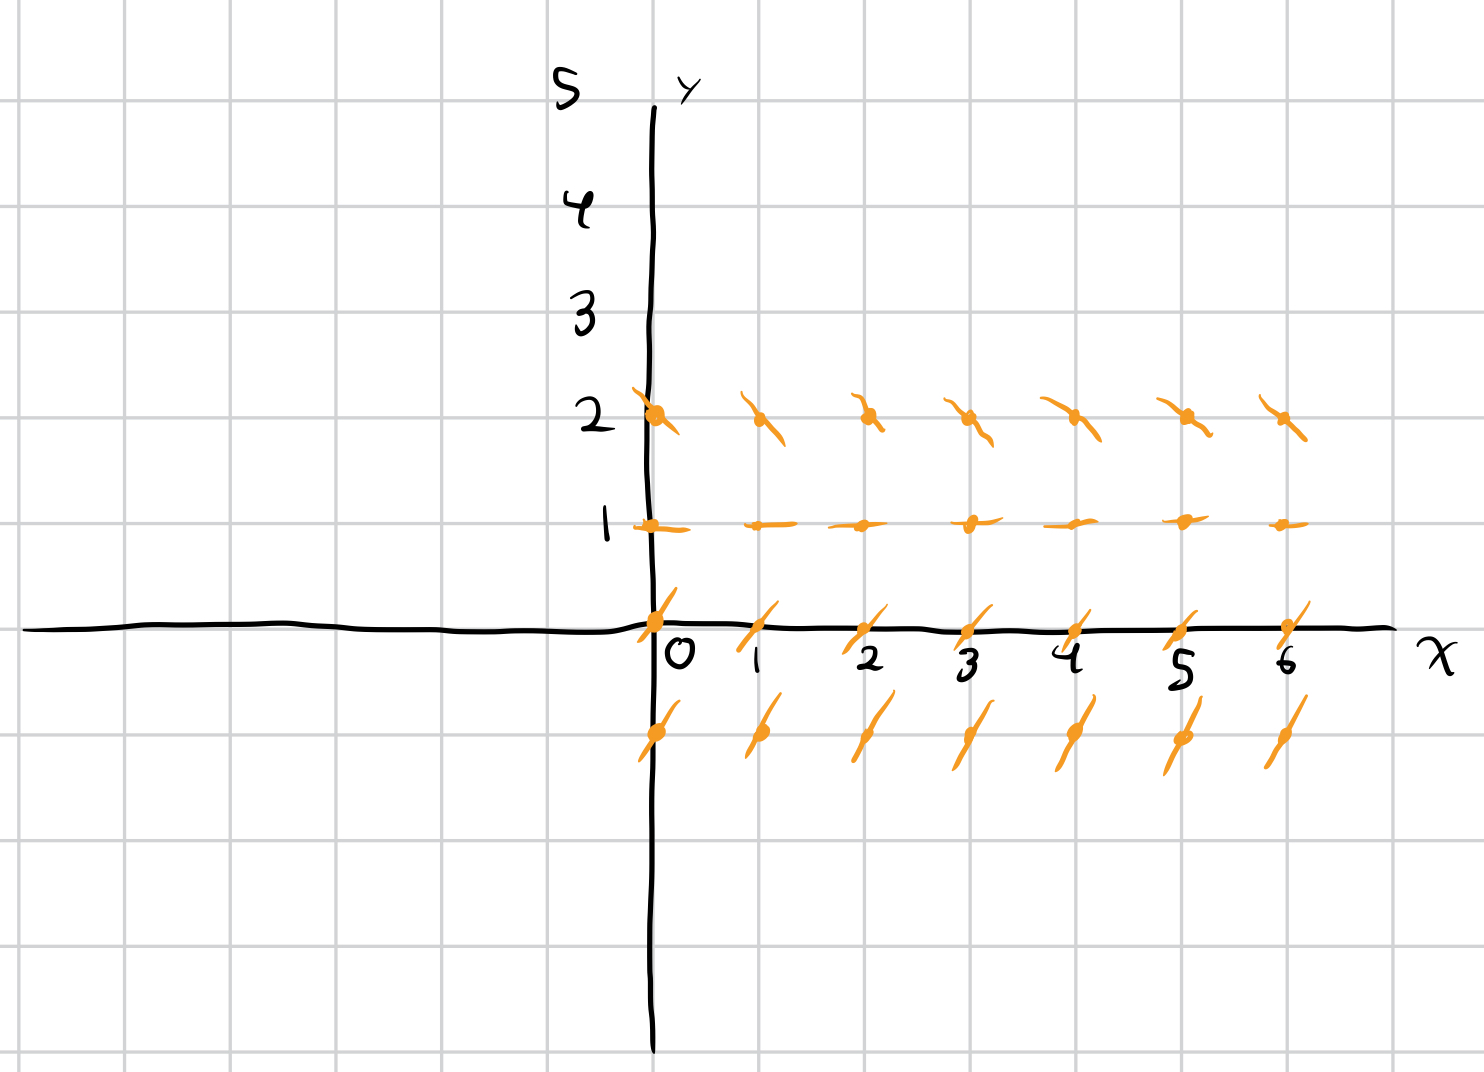
\includegraphics[width=7cm]{images/slope_field_2.png}
  \end{center}
  Qualitatively, we can see that
  \begin{itemize}
    \item at $y = 1$, all line segments are horizontal;
    \item for $y < 1$, all line segments have positive slope;
    \item for $y > 1$, all line segments have negative slope.
  \end{itemize}
  Using a computer, we can generate a better slope field:
  \begin{center}
    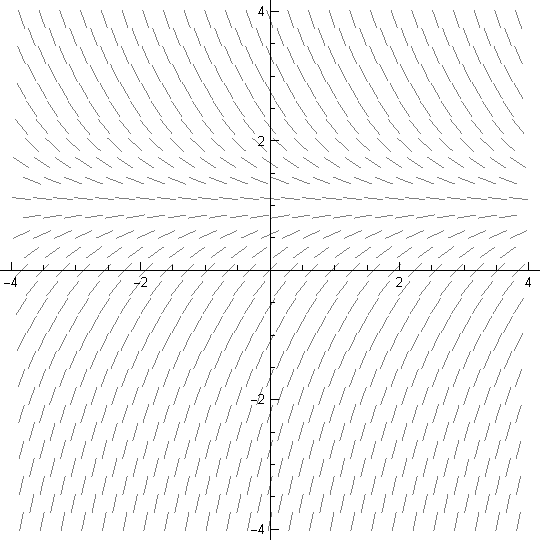
\includegraphics[width=10cm]{images/slopefieldnoexp.pdf}
%    \begin{tikzpicture}
%\begin{axis}[
%  axis x line*=center,
%  axis y line*=center,
%	xmin = -4, xmax = 4,
%	ymin = -4, ymax = 4,
%	zmin = 0, zmax = 1,
%	axis equal image,
%    xtick={-4,-3,-2,-1,0,1,2,3,4},
%    ytick={-4,-3,-2,-1,0,1,2,3,4},
%	view = {0}{90},
%]
%	\addplot3[
%    color=black!70!white,
%		quiver = {
%			u = {1/sqrt(1+(1-y)^2)},
%			v = {(1-y)/sqrt(1+(1-y)^2)},
%			scale arrows = 0.25,
%		},
%		-stealth,
%		domain = -4:4,
%		domain y = -4:4,
%	] {0};
%\end{axis}
%\end{tikzpicture}
  \end{center}
  Analytically, we solve the equation by separation of variables:
  \begin{align*}
    \frac{dy}{dx} &= 1-y\\
    \frac{dy}{1-y} &= dx\\
    \int_{}^{} \frac{1}{1-y}\:dy &= \int_{}^{} \:dx\\
    -\ln|1-y| &= x + C\\
    \left\vert 1-y \right\vert &= e^{-x-C_1}\\
    1-y &= \pm e^{-C_1}e^{-x}\\
    y &= 1-Ae^{-x}.
  \end{align*}
  With the initial condition of $y(0) = -1$, we get $y = 1-2e^{-x}$.

  \begin{center}
    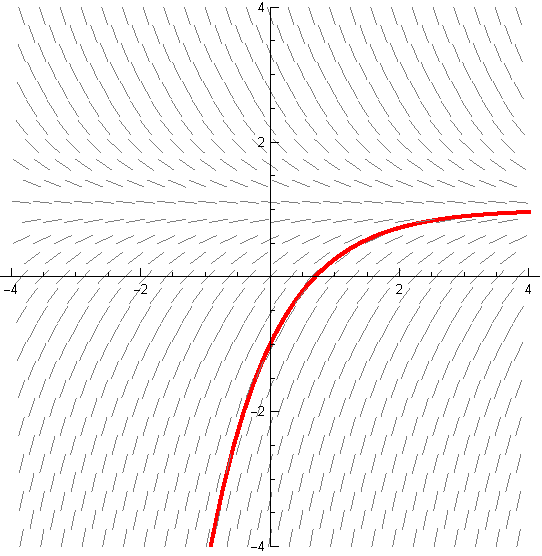
\includegraphics[width=10cm]{images/abcdef.pdf}
%    \begin{tikzpicture}
%\begin{axis}[
%  axis x line*=center,
%  axis y line*=center,
%	xmin = -4, xmax = 4,
%	ymin = -4, ymax = 4,
%	zmin = 0, zmax = 1,
%	axis equal image,
%	view = {0}{90},
%    xtick={-4,-3,-2,-1,0,1,2,3,4},
%    ytick={-4,-3,-2,-1,0,1,2,3,4},
%]
%	\addplot3[
%    color=black!20!white,
%		quiver = {
%			u = {1/sqrt(1+(1-y)^2)},
%			v = {(1-y)/sqrt(1+(1-y)^2)},
%			scale arrows = 0.25,
%		},
%		-stealth,
%		domain = -4:4,
%		domain y = -4:4,
%	] {0};
%\addplot[
%		-stealth,
%		domain = -4:4,
%    samples=100,
%    color=red
%    ]{1 - 2*pow(e,-x)};
%\end{axis}
%\end{tikzpicture}
  \end{center}
\end{example}
\subsection{Euler's Method}%
We want to approximate solutions to the differential equation $y' = f(x,y)$, $y(x_0) = y_0$. In the diagram, we can see the use of the slope field to calculate the approximate values of $\left(x_i,y_i\right)$.
\begin{center}
  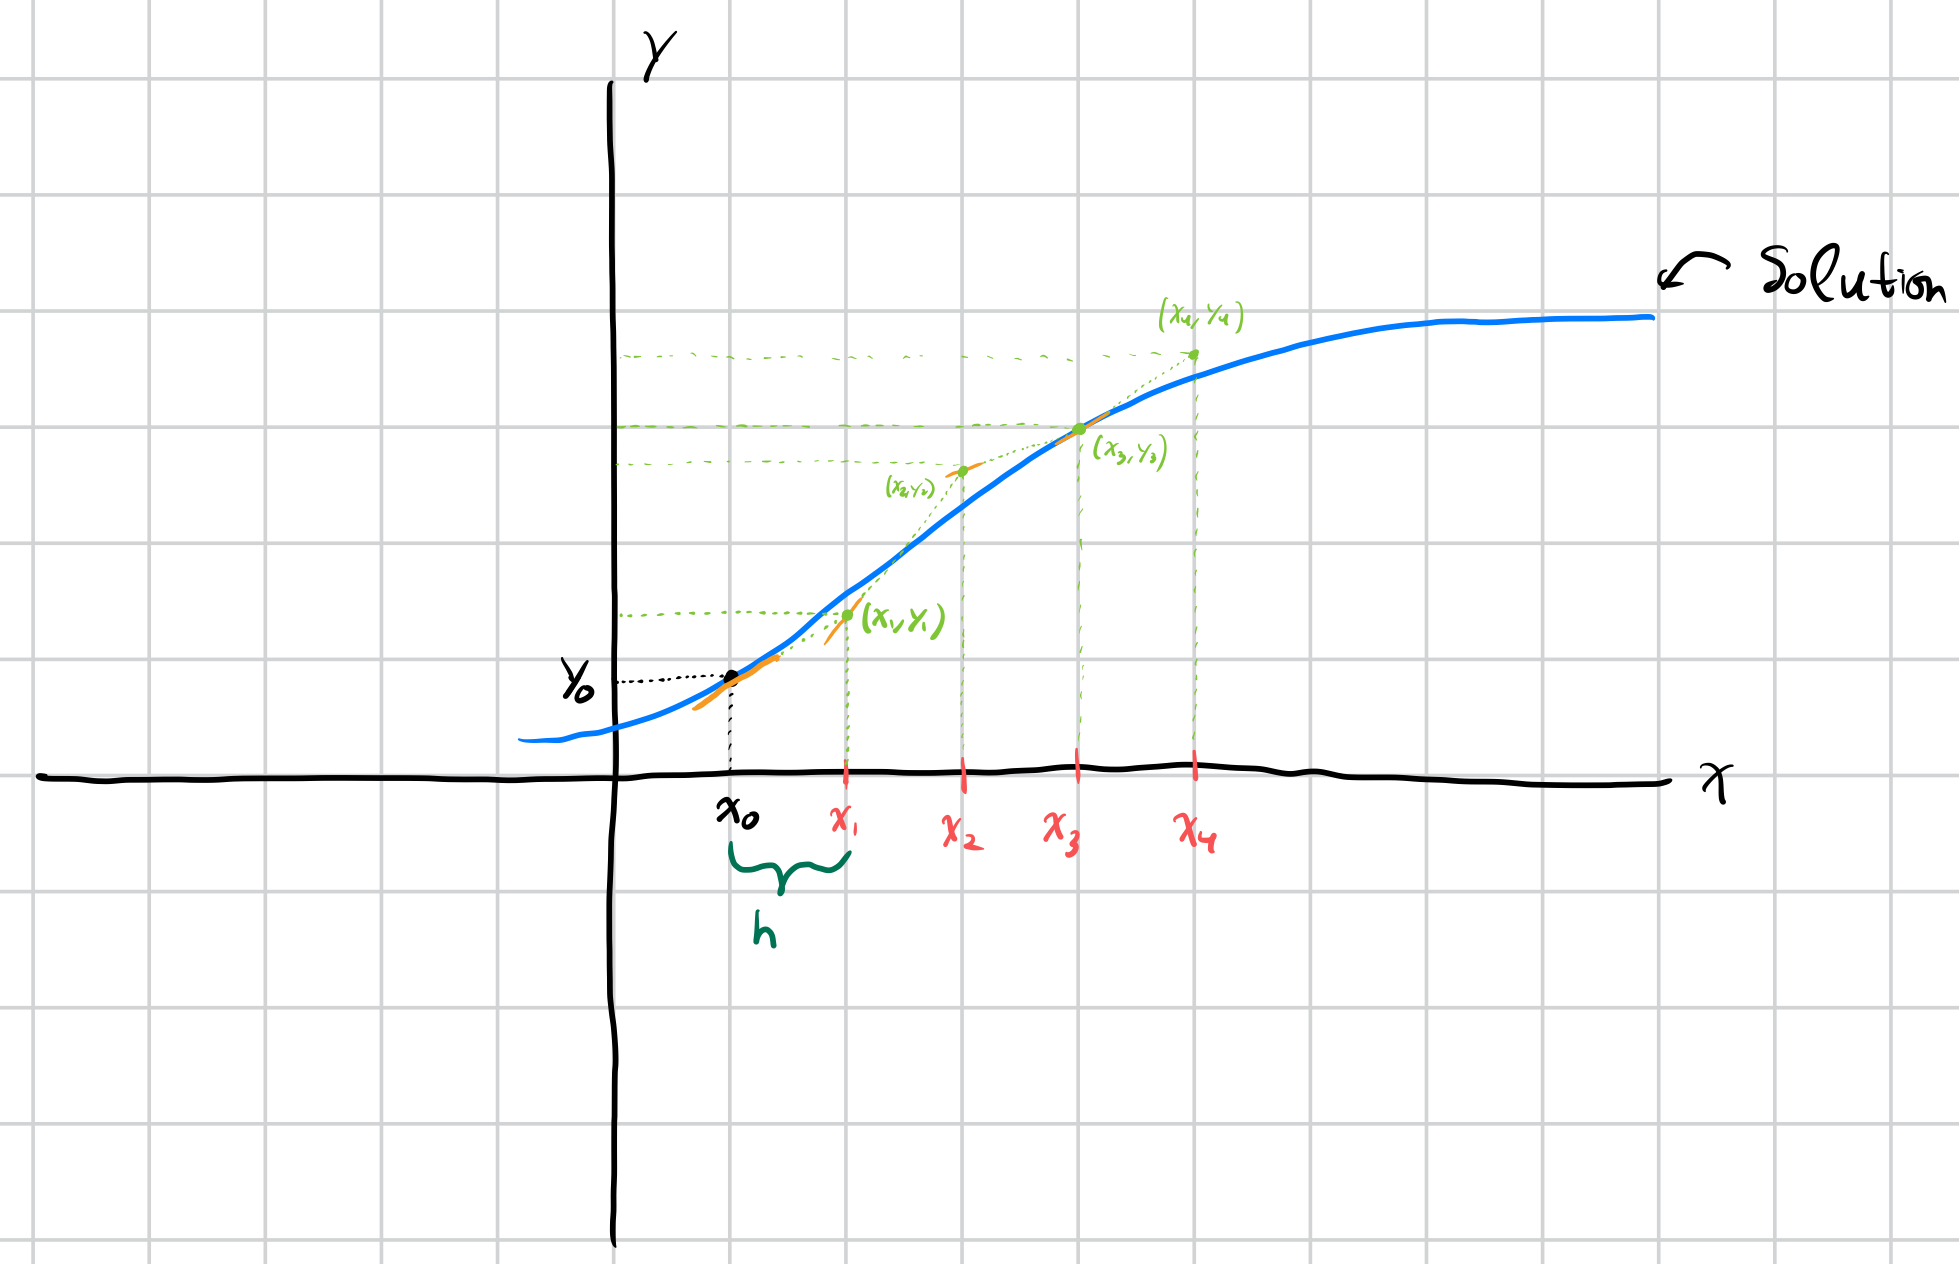
\includegraphics[width=15cm]{images/eulers_method_1.png}
\end{center}
\begin{method}[Euler's Method]
  To approximate the curve at $x_1 = x_0 + h$, we take the point-slope form:
  \begin{align*}
    \frac{y_1 - y_0}{\left(x_0 + h\right)-x_0} &= f\left(x_0,y_0\right)\\
    y_1 &= y_0 + hf\left(x_0,y_0\right).
  \end{align*}
  In general, we have
  \begin{align*}
    y_{k+1} &= y_k + hf\left(x_k,y_k\right).
  \end{align*}
\end{method}
\begin{example}
  Consider the differential equation $y' = 2y-1$. With the step size $\Delta x = h = 0.5$ and $y(0) = 1$, we can approximate $y(1)$ by
  \begin{center}
    \begin{tabular}{c|c|c|c}
      k & $x_k$ & $y_k$ & $f\left(x_k,y_k\right)$\\
      \hline
      $0$ & $1$ & 1 & 1\\
      $1$ & $1.5$ & $1.5$ & $2$\\
      $2$ & $2$ & $2.5$ & ---
    \end{tabular}
  \end{center}
  Thus, using Euler's method with a step size of $0.5$, we find that $y(1)\approx 2.5$. The table is read left to right, changing columns after calculating $f\left(x_k,y_k\right)$, then using it to calculate $y_{k+1}$.\newline

  Solving the differential equation analytically, we find
  \begin{align*}
    \frac{dy}{dx} &= 2y-1\\
    \int_{}^{} \frac{1}{2y-1}\:dy &= \int_{}^{} \:dx\\
    \frac{1}{2}\ln\left\vert 2y-1 \right\vert &= x + C_1\\
    \ln\left\vert 2y-1 \right\vert &= 2x + C_2\\
    \left\vert 2y-1 \right\vert &= e^{C_2}e^{2x}\\
    2y-1 &= \pm e^{C_2}e^{2x}\\
    y &= \frac{1}{2} + Ae^{2x}.
  \end{align*}
  Plugging in our initial condition, we find $A = \frac{1}{2}$, and the exact value of $y(1)$ is $\frac{1}{2} + \frac{1}{2}e^2$, which is approximately $4.1945$.\newline

  We can make our approximation via Euler's method better using a shorter step size.\newline

  For instance, by using a step size of 0.1, we find:
  \begin{center}
    \begin{tabular}{c|c|c|c}
      $k$ & $x_k$ & $y_k$ & $2y_k - 1$\\
      \hline
      $0$ & $0$ & $1$ & $1$\\
      1 & $0.1$ & $1.1$ & $1.2$ \\
      $2$ & $0.2$ & $1.22$& $1.44$ \\
      $3$ & $0.3$ & $1.364$& $1.728$\\
      $4$ & $0.4$ &$1.537$ & $2.07$\\
      $5$ & $0.5$ & $1.744$& $2.49$\\
      $6$ & $0.6$ & $1.993$ & $2.97$\\
      $7$ & $0.7$ & $2.29$ & $3.58$\\
      $8$ & $0.8$ & $2.65$ & $4.30$\\
      $9$ & $0.9$ & $3.08$& $5.16$\\
      $10$ & $1$ & $3.596$ & ---
    \end{tabular}
  \end{center}
  Note that our final approximation of $3.596$ is much better than the approximation under $h = 0.5$.\newline

  In order to understand if our estimate with Euler's method is an overestimate or underestimate, we use the second derivative test.
  \begin{align*}
    y' &= 2y - 1\\
    y'' &= 2y'\\
       &= 2\left(2y-1\right)\\
       &= 4y-2.
  \end{align*}
  In particular, our initial condition of $y(0) = 1$ suggests that $y'' = 2 > 0$, meaning Euler's method will return an underestimate (as the tangent lines will lie below the true curve).
\end{example}
\subsection{Existence and Uniqueness}%
Given an initial value problem
\begin{align*}
  \frac{dy}{dt} &= f(t,y)\\
  y\left(t_0\right) &= y_0,
\end{align*}
we ask the following two questions.
\begin{enumerate}[(1)]
  \item When does a solution to this initial value problem exist?
  \item If it does exists, is the solution unique?
\end{enumerate}
\begin{example}
  Consider the polynomial
  \begin{align*}
    \underbrace{2x^5 - 10x + 5}_{f} = 0,
  \end{align*}
  and suppose want to find solutions to this equation.\newline

  Notice that $f$ is continuous on $[-1,1]$, with $f(-1) = 13$ and $f(1) = 3$.\newline

  By the Intermediate Value Theorem, this must mean $f$ takes on the value of $0$ at at least one value between $x=-1$ and $x=1$.
\end{example}
\begin{theorem}[Existence and Uniqueness]
  Let $R$ be a rectangular region in the $t,y$-plane containing the point $\left(t_0,y_0\right)$ in the interior of $R$. In particular, $R = \set{(t,y)\mid a<t<b, c < y < d}$, and $\left(t_0,y_0\right)\in R$.\newline

  If $f(t,y)$ and $\pd{f}{y}$ are continuous on $R$, then there exists $\ve > 0$ and a unique function $y(t)$ defined on some neighborhood $t_0 - \ve < t < t_0 + \ve$ contained in $a < t < b$ such that $y(t)$ is a solution to the initial value problem
  \begin{align*}
    \frac{dy}{dt} &= f(t,y)\\
    y\left(t_0\right) &= y_0.
  \end{align*}
\end{theorem}
Note the two major conditions here:
\begin{itemize}
  \item the continuity of $f$ on $R$; this guarantees existence\\
  \item the continuity of $\pd{f}{y}$ on $R$; this guarantees uniqueness.
\end{itemize}
\begin{center}
  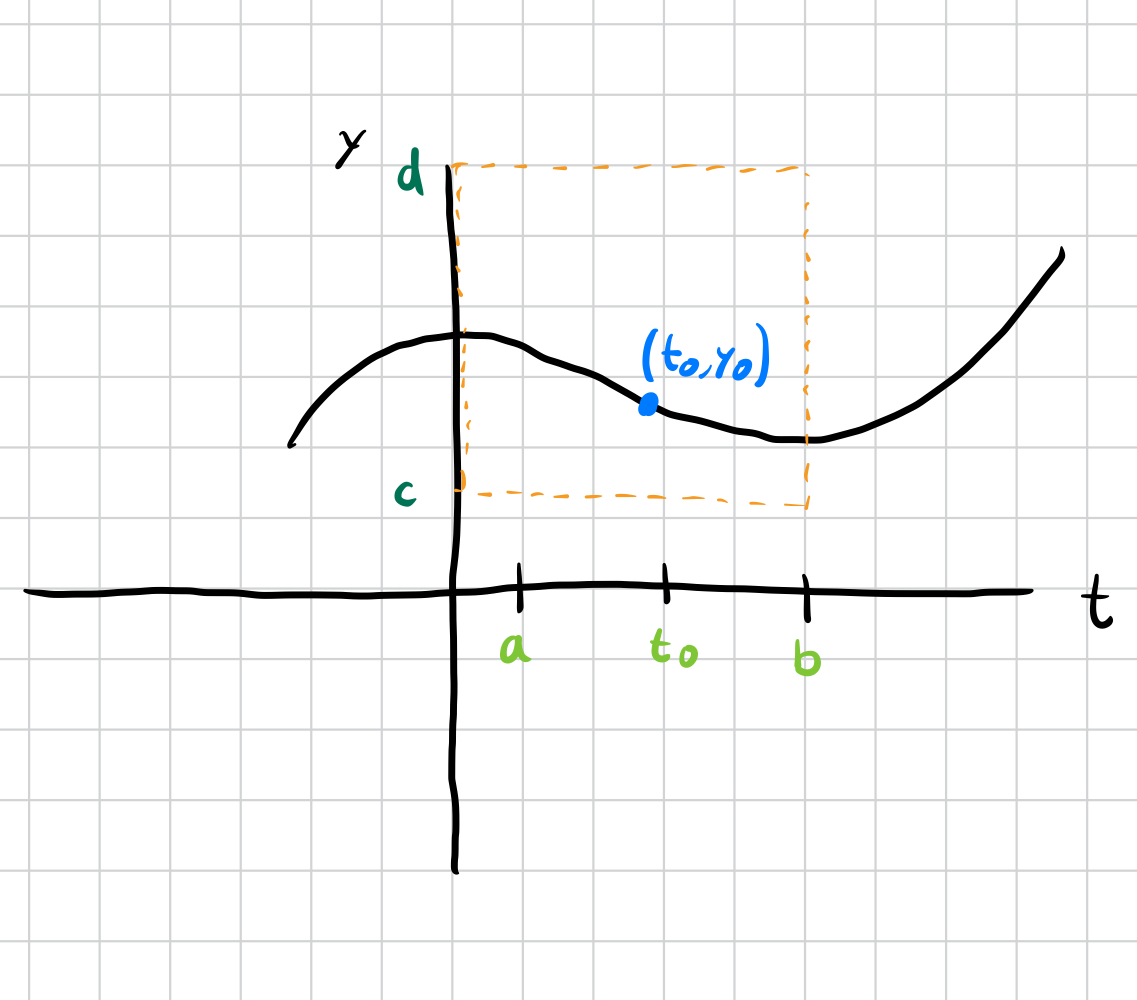
\includegraphics[width=7cm]{images/existence_uniqueness.png}
\end{center}
If one of the conditions is not satisfied, we may have
\begin{itemize}
  \item exactly one solution;
  \item many solutions;
  \item no solutions.
\end{itemize}
\begin{example}
  Consider the differential equation
  \begin{align*}
    \frac{dy}{dt} &= t^2 y^{1/2},
  \end{align*}
  and $y(0) = 0$.\newline

  We have $f(t,y) = t^2 y^{1/2}$. We have
  \begin{align*}
    \pd{f}{y} &= \frac{1}{2}t^2y^{-1/2}\\
              &= \frac{t^2}{2\sqrt{y}}.
  \end{align*}
  We can see that $f$ is continuous at $(0,0)$, but $\pd{f}{y}$ is not continuous at $(0,0)$.\newline

  Additionally, since $f$ is not defined for $y < 0$, we cannot place $(0,0)$ in the interior of any region on the $t,y$-plane.\newline

  Therefore, we cannot use the existence and uniqueness theorem on $f$.\newline

  Going forward analytically, we start with the equilibrium condition $y(t) = 0$. Using separation of variables, we have
  \begin{align*}
    \frac{dy}{dt} &= t^2y^{1/2}\\
    \int\frac{dy}{y^{1/2}} &= \int_{}^{} t^2\:dt\\
    2y^{1/2} &= \frac{t^3}{3} + C\\
    y &= \left(\frac{t^3}{6} + K\right)^{2}\\
    0 &= \left(\frac{(0)^3}{6} + K\right)^{2}\\
    K &= 0\\
    \intertext{meaning we also have a solution of}
    y(t) &= \left(\frac{t^3}{6}\right)^{2}\\
         &= \frac{t^6}{36}.
  \end{align*}
\end{example}
\begin{example}
  Let $\frac{dy}{dt} = t^2y^{1/2}$ with the (new) initial condition of $y(2) = 1$.\newline

  In particular, we can see that not only is $f(t,y)$ continuous at $0$, but so too is $\pd{f}{y}$, and there exists a region about the point $(2,1)$ such that $f$ and $\pd{f}{y}$ are continuous.\newline

  Thus, by the existence and uniqueness theorem, there exists exactly one solution to this initial value problem.
\end{example}
\begin{example}
  Let $\frac{dy}{dt} = 1 + y^2$, with the initial condition $y(0) = 0$.\newline

  We have $f(t,y) = 1 + y^2$, $\pd{f}{y} = 2y$; both of these functions are continuous on the $t,y$-plane. Thus, by the existence and uniqueness theorem, there exists a unique solution to this initial value problem.\newline

  We solve by separation of variables:
  \begin{align*}
    \frac{dy}{dt} &= 1 + y^2\\
    \int_{}^{} \frac{1}{1+y^2}\:dy &= \int_{}^{} \:dt\\
    \arctan(y) &= t + C\\
    y &= \tan\left(t + C\right)\\
    0 &= \tan\left(0 + C\right)\\
    0 &= \tan\left(C\right).
  \end{align*}
  We can let $C = 0$, meaning we have the solution
  \begin{align*}
    y(t) &= \tan t.
  \end{align*}
  \begin{center}
    \begin{tikzpicture}
\begin{axis}[
  axis x line*=center,
  axis y line*=center,
	xmin = -4, xmax = 4,
	ymin = -4, ymax = 4,
	axis equal image,
    xtick={-4,-3,-2,-1,0,1,2,3,4},
    ytick={-4,-3,-2,-1,0,1,2,3,4},
]
%	\addplot3[
%    color=black!20!white,
%		quiver = {
%			u = {1/sqrt(1+(1-y)^2)},
%			v = {(1-y)/sqrt(1+(1-y)^2)},
%			scale arrows = 0.25,
%		},
%		-stealth,
%		domain = -4:4,
%		domain y = -4:4,
%	] {0};
\addplot[
		-stealth,
		domain = -1.5:1.5,
    samples=100,
    color=red
    ]{tan(deg(x))};
\end{axis}
\end{tikzpicture}
  \end{center}
\end{example}
\begin{example}[Application of the Uniqueness Theorem]
  Suppose $f(t,y)$ satisfies the conditions for uniqueness.\newline

  Assume $y_1(t)$ and $y_2(t)$ are solutions of the differential equation $\frac{dy}{dt} = f(t,y)$.\newline

  If these solutions intersect at some $t = t_0$, then $y_1(t)$ and $y_2(t)$ are solutions to this new initial value problem of
  \begin{align*}
    \diff{y}{t} &= f(t,y)\\
    y\left(t_0\right) &= y_1\left(t_0\right) = y_2\left(t_0\right).
  \end{align*}
  Since $f$ satisfies the uniqueness theorem, it be the case that $y_1(t) = y_2(t)$.\newline

  In particular, this means that solutions to differential equations that satisfy the uniqueness conditions cannot intersect. In other words, solutions cannot equal each other at the same ``place'' at the same ``time.''
\end{example}
\begin{example}
  Consider the initial value problem
  \begin{align*}
    \frac{dy}{dt} &= \frac{2y}{t}\\
    y(1) &= 1.
  \end{align*}
  We have $f(t,y) = \frac{2y}{t}$, $\pd{f}{y} = \frac{2}{t}$. We can see that $f$ and $\pd{f}{y}$ are continuous at $(1,1)$, as well as a given region with $(1,1)$ in its interior (since continuity is only lost when $t = 0$).\newline

  Thus, there exists a unique solution to this initial value problem. We can solve the equation via separation of variables:
  \begin{align*}
    \frac{dy}{dt} &= \frac{2y}{t}\\
    \int_{}^{} \frac{1}{2y}\:dy &= \int_{}^{} \frac{1}{t}\:dt\\
    \frac{1}{2}\ln|y| &= \ln|t| + C\\
    \ln|y| &= 2\ln|t| + 2C\\
    |y| &= e^{2\ln|t|}e^{2C}\\
    y &= \pm e^{2C}t^2\\
    y &= Kt^2
  \end{align*}
  We have the initial condition $y(1) = 1$, meaning we have the solution $y(t) = t^2$.\newline

  Notice that as a function, the domain of $y$ is $\R$, but as a solution, we cannot have $t = 0$, meaning that the domain of $y(t) = t^2$ \textit{as a solution} is $t > 0$.
\end{example}
\subsection{Equilibria and Phase Lines}%
Given a differential equation
\begin{align*}
  \frac{dy}{dt} = f(t,y),
\end{align*}
we can use slope fields and Euler's method to find an approximate solution, as well as various analytic methods to find a definite solution.\newline

Given an autonomous differential equation, though,
\begin{align*}
  \frac{dy}{dt} &= f(y),
\end{align*}
particularly one with $f,\pd{f}{y}$ continuous, we can use some deeper analysis.\newline

In particular, for constant $y$, the slope at any point $(t,y)$ will be the same as at any other $(t,y)$. This means we can analyze the behavior of \textit{the entire solution} based on one particular line.
\begin{method}[Equilibrium Analysis for Autonomous Differential Equations]\hfill
  \begin{enumerate}[(1)]
    \item Solve $f(y) = 0$ to find the equilibrium solutions.
    \item Analyze the behavior of $f(y)$ around the equilibrium points.
      \begin{itemize}
        \item Draw a particular line, known as a phase line, with positive $t$.
        \item Determine if $f(y)$ is positive or negative between equilibrium points.
        \item If $f(y) > 0$, then the solution is increasing in this region, and if $f(y) < 0$, the solution is decreasing in this region.
      \end{itemize}
  \end{enumerate}
\end{method}
\begin{example}
  Let
  \begin{align*}
    \frac{dy}{dt} &= (1-y)y.
  \end{align*}
  Thus, we have $f(y) = (1-y)y$, meaning $y(1-y) = 0$ for $y=0$ and $y=1$.\newline

  For $ y = 2$, we have $f(2) = -2 < 0$, for $y = 0.5$, $f(y) = 0.25 > 0$, and $f(-1) = -2 < 0$. Thus, our equilibrium analysis looks like the following:
  \begin{center}
    \begin{tikzpicture}
      \draw (0,-3) -- (0,3);
      \filldraw (0,1) circle (2pt)
        (0,0) circle (2pt);
      \node[anchor = west] at (0,1) {$y = 1$};
      \node[anchor = west] at (0,0) {$y = 0$};
      \draw[->] (0,2) -- (0,1.5);
      \draw[->] (0,0.25) -- (0,0.5);
      \draw[->] (0,-1) -- (0,-1.5);
    \end{tikzpicture}
  \end{center}
  \begin{center}
    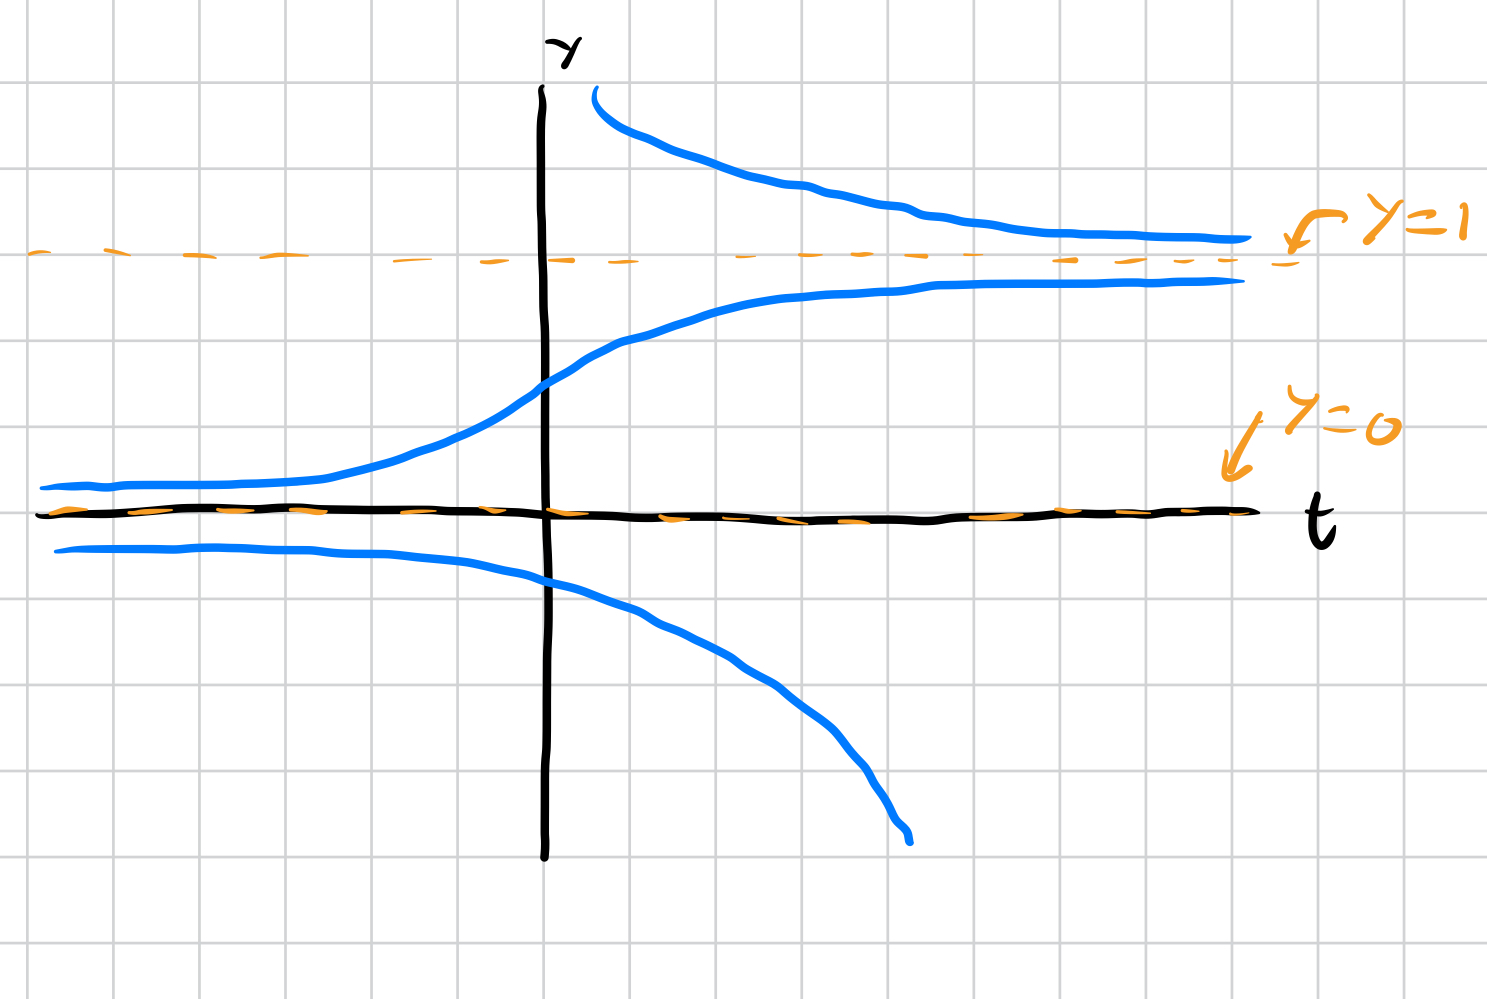
\includegraphics[width=10cm]{images/equilibrium_analysis.png}
  \end{center}
\end{example}
\begin{definition}[Classificiation of Equilibrium Points]\hfill
  \begin{enumerate}[(1)]
    \item An equilibrium point at $y=c$ is called a sink if all the solutions with the initial condition near $y = c$ approach $c$ as $t$ approaches $\infty$.
      \begin{itemize}
        \item On the phase line, $f(y)$ goes from $+$ to $-$ on the phase line as $y$ goes from $c - \ve$  to $c + \ve$.
      \end{itemize}
    \item An equilibrium point at $y=c$ is called a source if all the solutions with the initial conditions near $y = c$ move away from $c$ as $t$ approaches $\infty$.
      \begin{itemize}
        \item On the phase line, $f(y)$ goes from $-$ to $+$ on the phase line as $y$ goes from $c-\ve$ to $c + \ve$.
      \end{itemize}
    \item Every equilibrium point that is neither a source nor a sink is called a node.
      \begin{itemize}
        \item On the phase space, $f(y)$ maintains the same sign as $y$ goes from $c - \ve$ to $c + \ve$.
      \end{itemize}
  \end{enumerate}
\end{definition}
\begin{example}[Logistic Population Model]
Recall that the logistic population model is
\begin{align*}
  \frac{dy}{dt} &= \underbrace{k\left(1-\frac{y}{m}\right)y}_{f(y)},
\end{align*}
with the conditions of $k > 0$, $m > 0$. We want to draw a phase line for this model.\newline

The equilibrium solutions are at $y=0$ and $y = m$. We draw our phase line with its equilibrium points as
\begin{center}
  \begin{tikzpicture}
    \draw (0,2) -- (0,-1);
    \filldraw (0,0) circle (2pt)
    (0,1) circle (2pt);
    \node[anchor = west] at (0,0) {$y=0$};
    \node[anchor = west] at (0,1) {$y=m$};
  \end{tikzpicture}
\end{center}
To find out what happens in between, we choose
\begin{itemize}
  \item $y = -1$; $f(y) < 0$.
  \item $y = m/2$; $f(y) > 0$.
  \item $y = 2m$; $f(y) < 0$.
\end{itemize}
Therefore, our phase line is
\begin{center}
  \begin{tikzpicture}
    \draw (0,2) -- (0,-1);
    \filldraw (0,0) circle (2pt)
    (0,1) circle (2pt);
    \node[anchor = west] at (0,0) {$y=0$};
    \node[anchor = west] at (0,1) {$y=m$};
    \draw[->](0,2) -- (0,1.5);
    \draw[->](0,0.25) -- (0,0.5);
    \draw[->](0,-0.25) -- (0,-0.5);
    \end{tikzpicture}
\end{center}
\end{example}
\begin{theorem}[Linearization]
  Suppose $y_0$ is an equilibrium point of the differential equation $\frac{dy}{dt} = f(y)$, where $f(y)$ is a continuously differentiable function. Then,
  \begin{itemize}
    \item if $f'\left(y_0\right) < 0$, then $y_0$ is a sink;
    \item if $f'\left(y_0\right) > 0$, then $y_0$ is a source;
    \item if $f'\left(y_0\right) = 0$, then we do not have enough information to determine the type of $y_0$.
  \end{itemize}
\end{theorem}
\begin{remark}
  In order to do an equilibrium analysis given a graph of $f(y)$, we identify all our equilibrium points by finding the roots of $f$, then examining the slope of $f$ at each of the identified equilibrium points.
\end{remark}
\begin{example}
  Suppose
  \begin{align*}
    \frac{dy}{dt} &= \left(y-1\right)\left(y^5 - 7y^4 + 3y^3 + 8y^2 - 11\right).
  \end{align*}
  We want to classify the equilibrium point $y=1$. In order to do this, we find its derivative:
  \begin{align*}
    \pd{f}{y} &= \left(y^5 - 7y^4 + 3y^3 + 8y^2 - 11\right) + \left(y-1\right)\left(5y^4 - 28y^3 + 9y^2 + 16y\right).
  \end{align*}
  Evaluating
  \begin{align*}
    \pd{f}{y}\bigr\vert_{y=1} &= -6,
  \end{align*}
  meaning our equilibrium point at $y=1$ is a sink.
\end{example}
\subsection{Bifurcations}%
Consider a first-order differential equation
\begin{align*}
  y' &= f\left(y,c\right).
\end{align*}
The value $c\in \R$ means this differential equation is actually a family of differential equations. We say $c$ is a parameter for the differential equation.
\begin{example}[A Parametrized in a Differential Equation]
  Consider the differential equation modelling the population of fish in a pond, denoted
  \begin{align*}
    \frac{dP}{dt} &= kP\left(1-\frac{P}{M}\right) - h.
  \end{align*}
  Here, $k$ is a constant, while $h$ is a parameter denoting the harvesting rate.
\end{example}
In general, as $c$ varies in our parametrized differential equation, an equilibrium solution may split into two equilibrium solutions disappear entirely.
\begin{example}
  Consider the family
  \begin{align*}
    \frac{dy}{dt} &= y^2 - c.
  \end{align*}
  The equilibrium solutions occur when $y^2 - c = 0$, meaning that for $c > 0$, our equilibrium solutions are at $y=\pm\sqrt{c}$. If $c = 0$, then $y=0$ is an equilibrium solution, and if $c < 0$, there are no equilibrium solutions.\newline

  We can see that $c = 0$ is a bifurcation point.\newline

  For $c = -1$, our differential equation is $\frac{dy}{dt} = y^2 + 1$.
  \begin{center}
    \begin{tikzpicture}
      \draw[->] (0,-1)-- (0,0);
      \draw (0,-2) -- (0,2);
    \end{tikzpicture}
  \end{center}
  For $c = 0$, our differential equation is $\frac{dy}{dt} = y^2$.
  \begin{center}
    \begin{tikzpicture}
      \draw[->] (0,0)-- (0,1);
      \draw[->] (0,-2)-- (0,-1);
      \filldraw (0,0) circle (2pt);
      \node[anchor=west] at (0,0) {$y=0$};
      \draw (0,-2) -- (0,2);
    \end{tikzpicture}
  \end{center}
  For $c = 1$, our differential equation is $\frac{dy}{dt} = y^2 - 1$.
  \begin{center}
    \begin{tikzpicture}
      \draw[->] (0,0.5)-- (0,0);
      \draw[->] (0,-2)-- (0,-1.5);
      \draw[->] (0,1) -- (0,1.5);
      \filldraw (0,1) circle (2pt);
      \filldraw (0,-1) circle (2pt);
      \node[anchor=west] at (0,-1) {$y=-1$};
      \node[anchor=west] at (0,1) {$y=1$};
      \draw (0,-2) -- (0,2);
    \end{tikzpicture}
  \end{center}
  The bifurcation diagram is as follows. 
  \begin{center}
    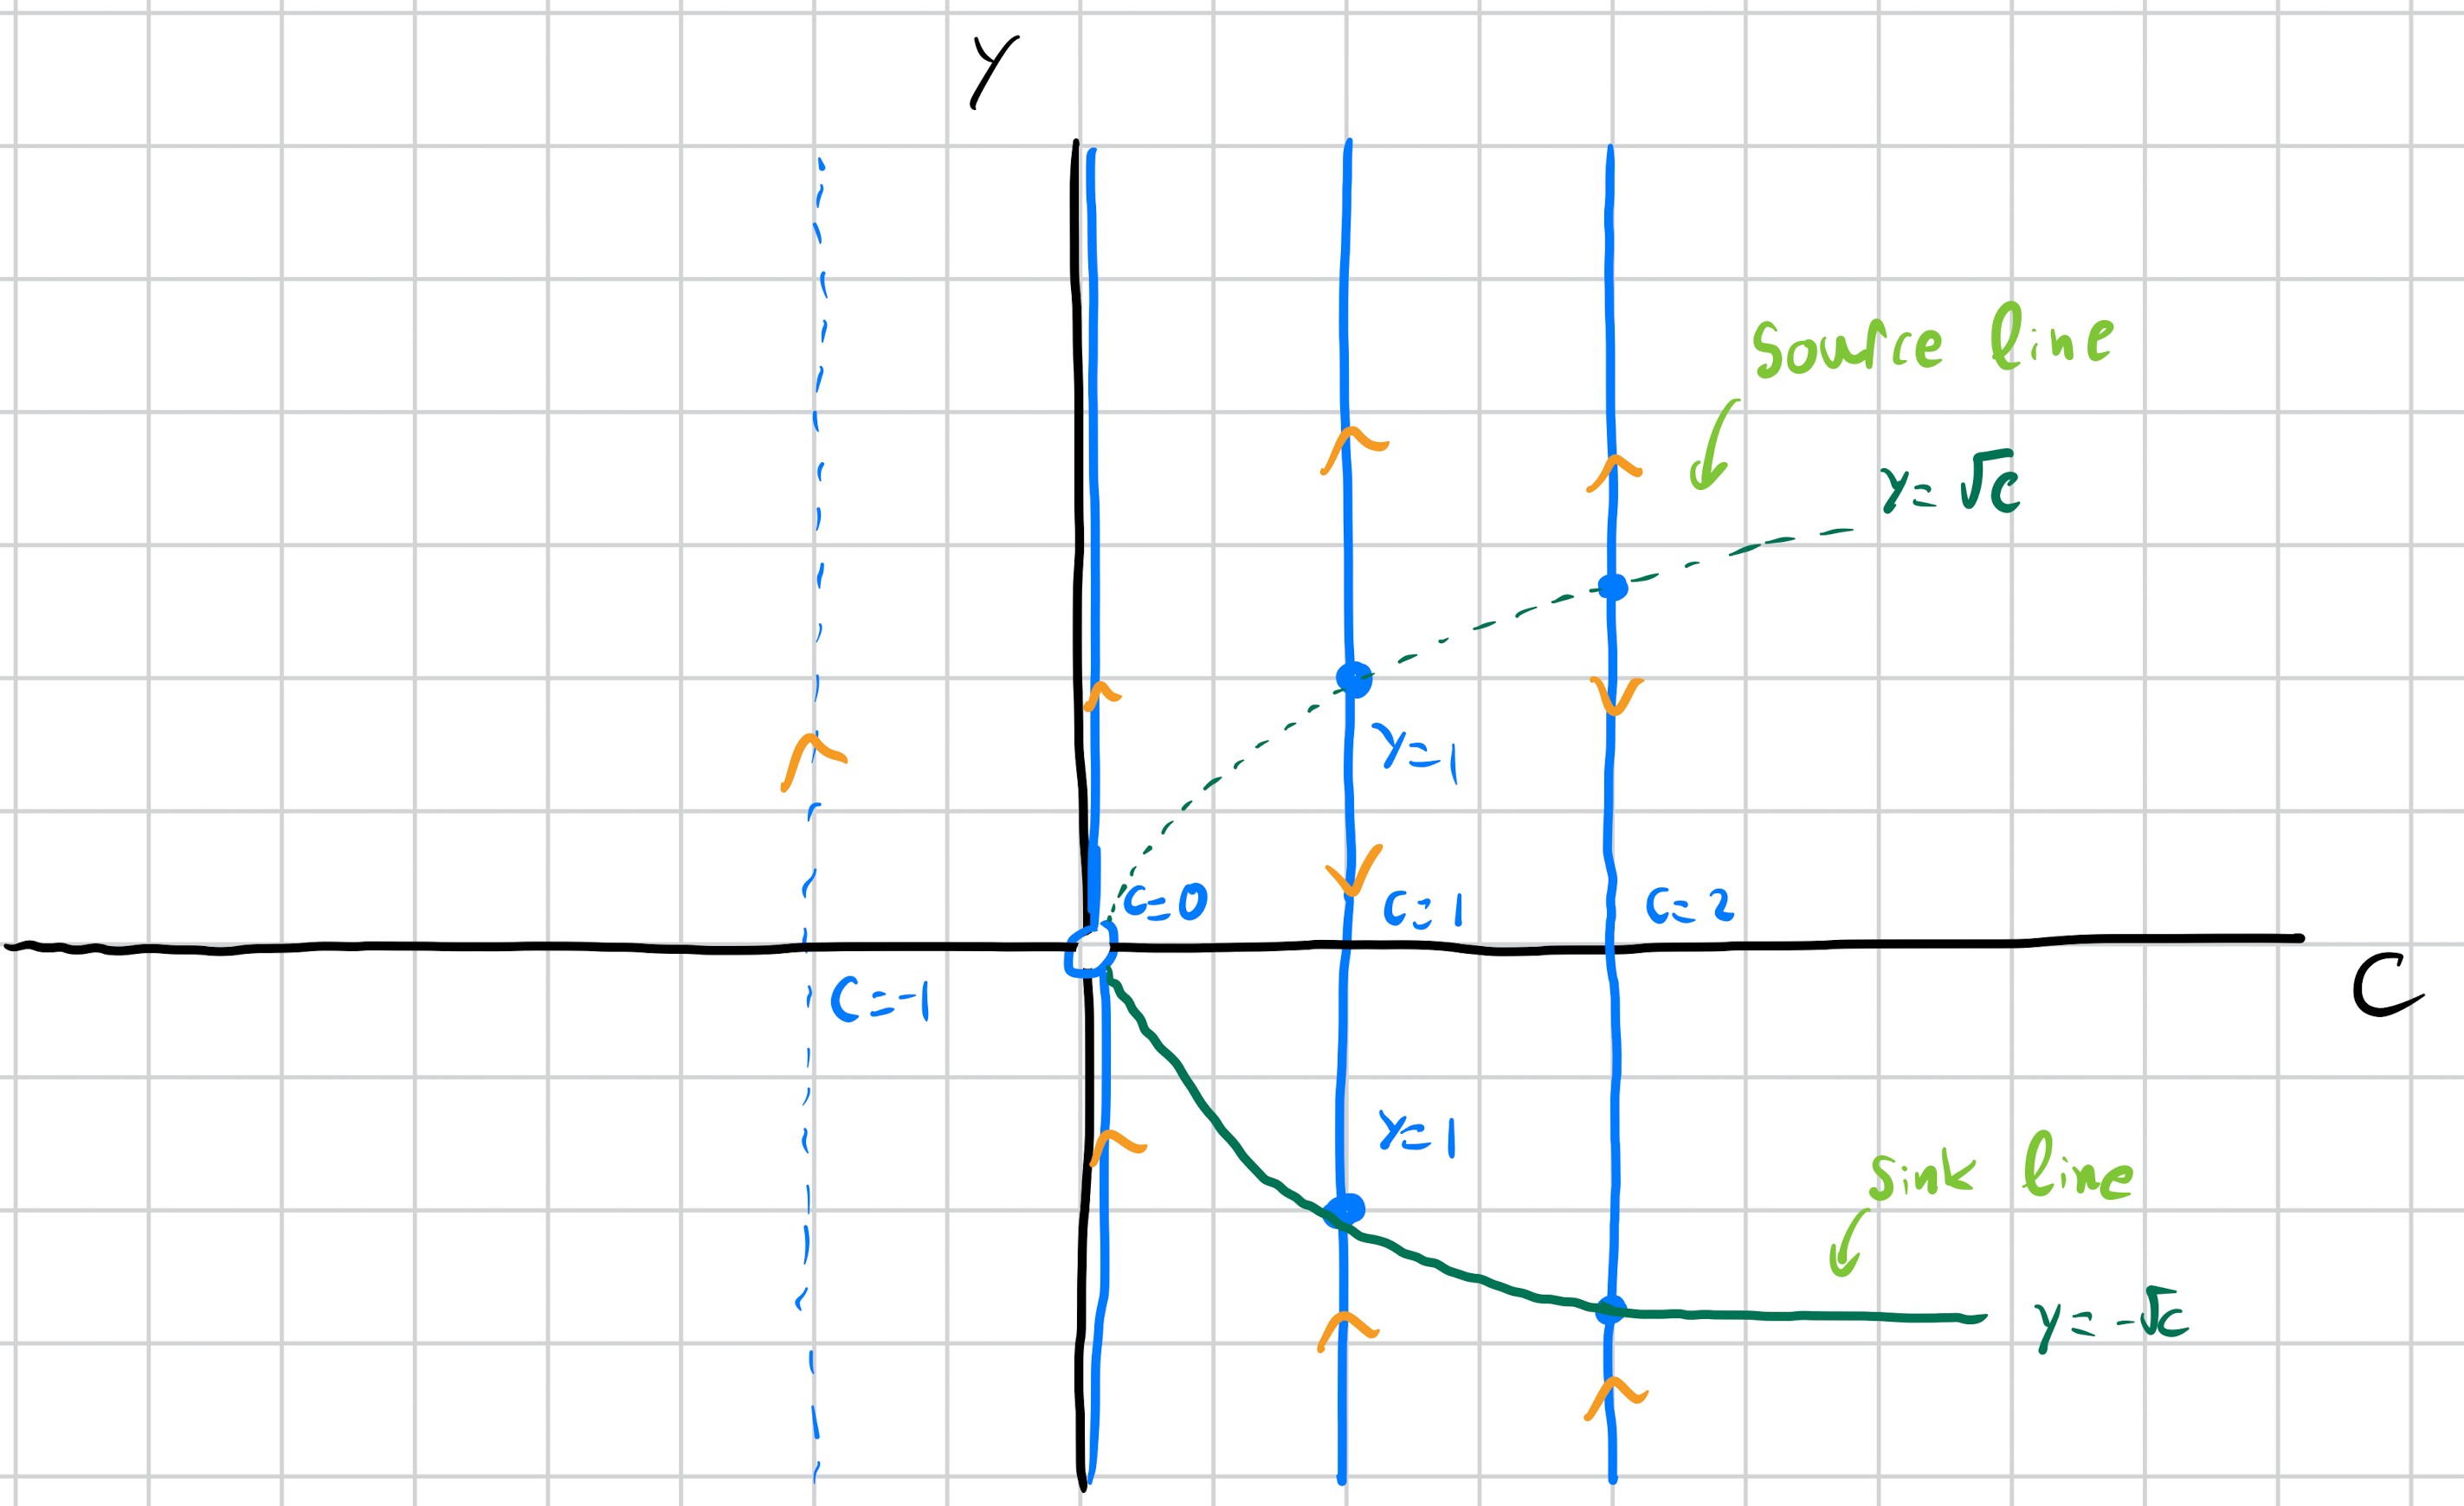
\includegraphics[width=12cm]{images/bifurcation_diagram.png}
  \end{center}
  Notice that the bifurcation point occurs when the source line and sink line meet.
\end{example}
\begin{example}[Solving a Population Model]
  Consider
  \begin{align*}
    \frac{dP}{dt} &= \underbrace{P\left(1 - P\right) - h}_{=f(P,h)}
  \end{align*}
  Equilibrium solutions occur at
  \begin{align*}
    P\left(1-P\right) - h &= 0\\
    P^2 - P + h &= 0\\
    P^2 - P + \frac{1}{4} &= \frac{1}{4} - h\\
    \left(P-\frac{1}{2}\right)^2 &= \frac{1}{4} - h\\
    P &= \frac{1}{2} \pm \sqrt{\frac{1}{4} - h}.
  \end{align*}
  Based on the values of $h$, we have no equilibrium solutions for $h > \frac{1}{4}$, one equilibrium solution for $h = \frac{1}{4}$, and two equilibrium solutions for $h < \frac{1}{4}$.
  \begin{center}
    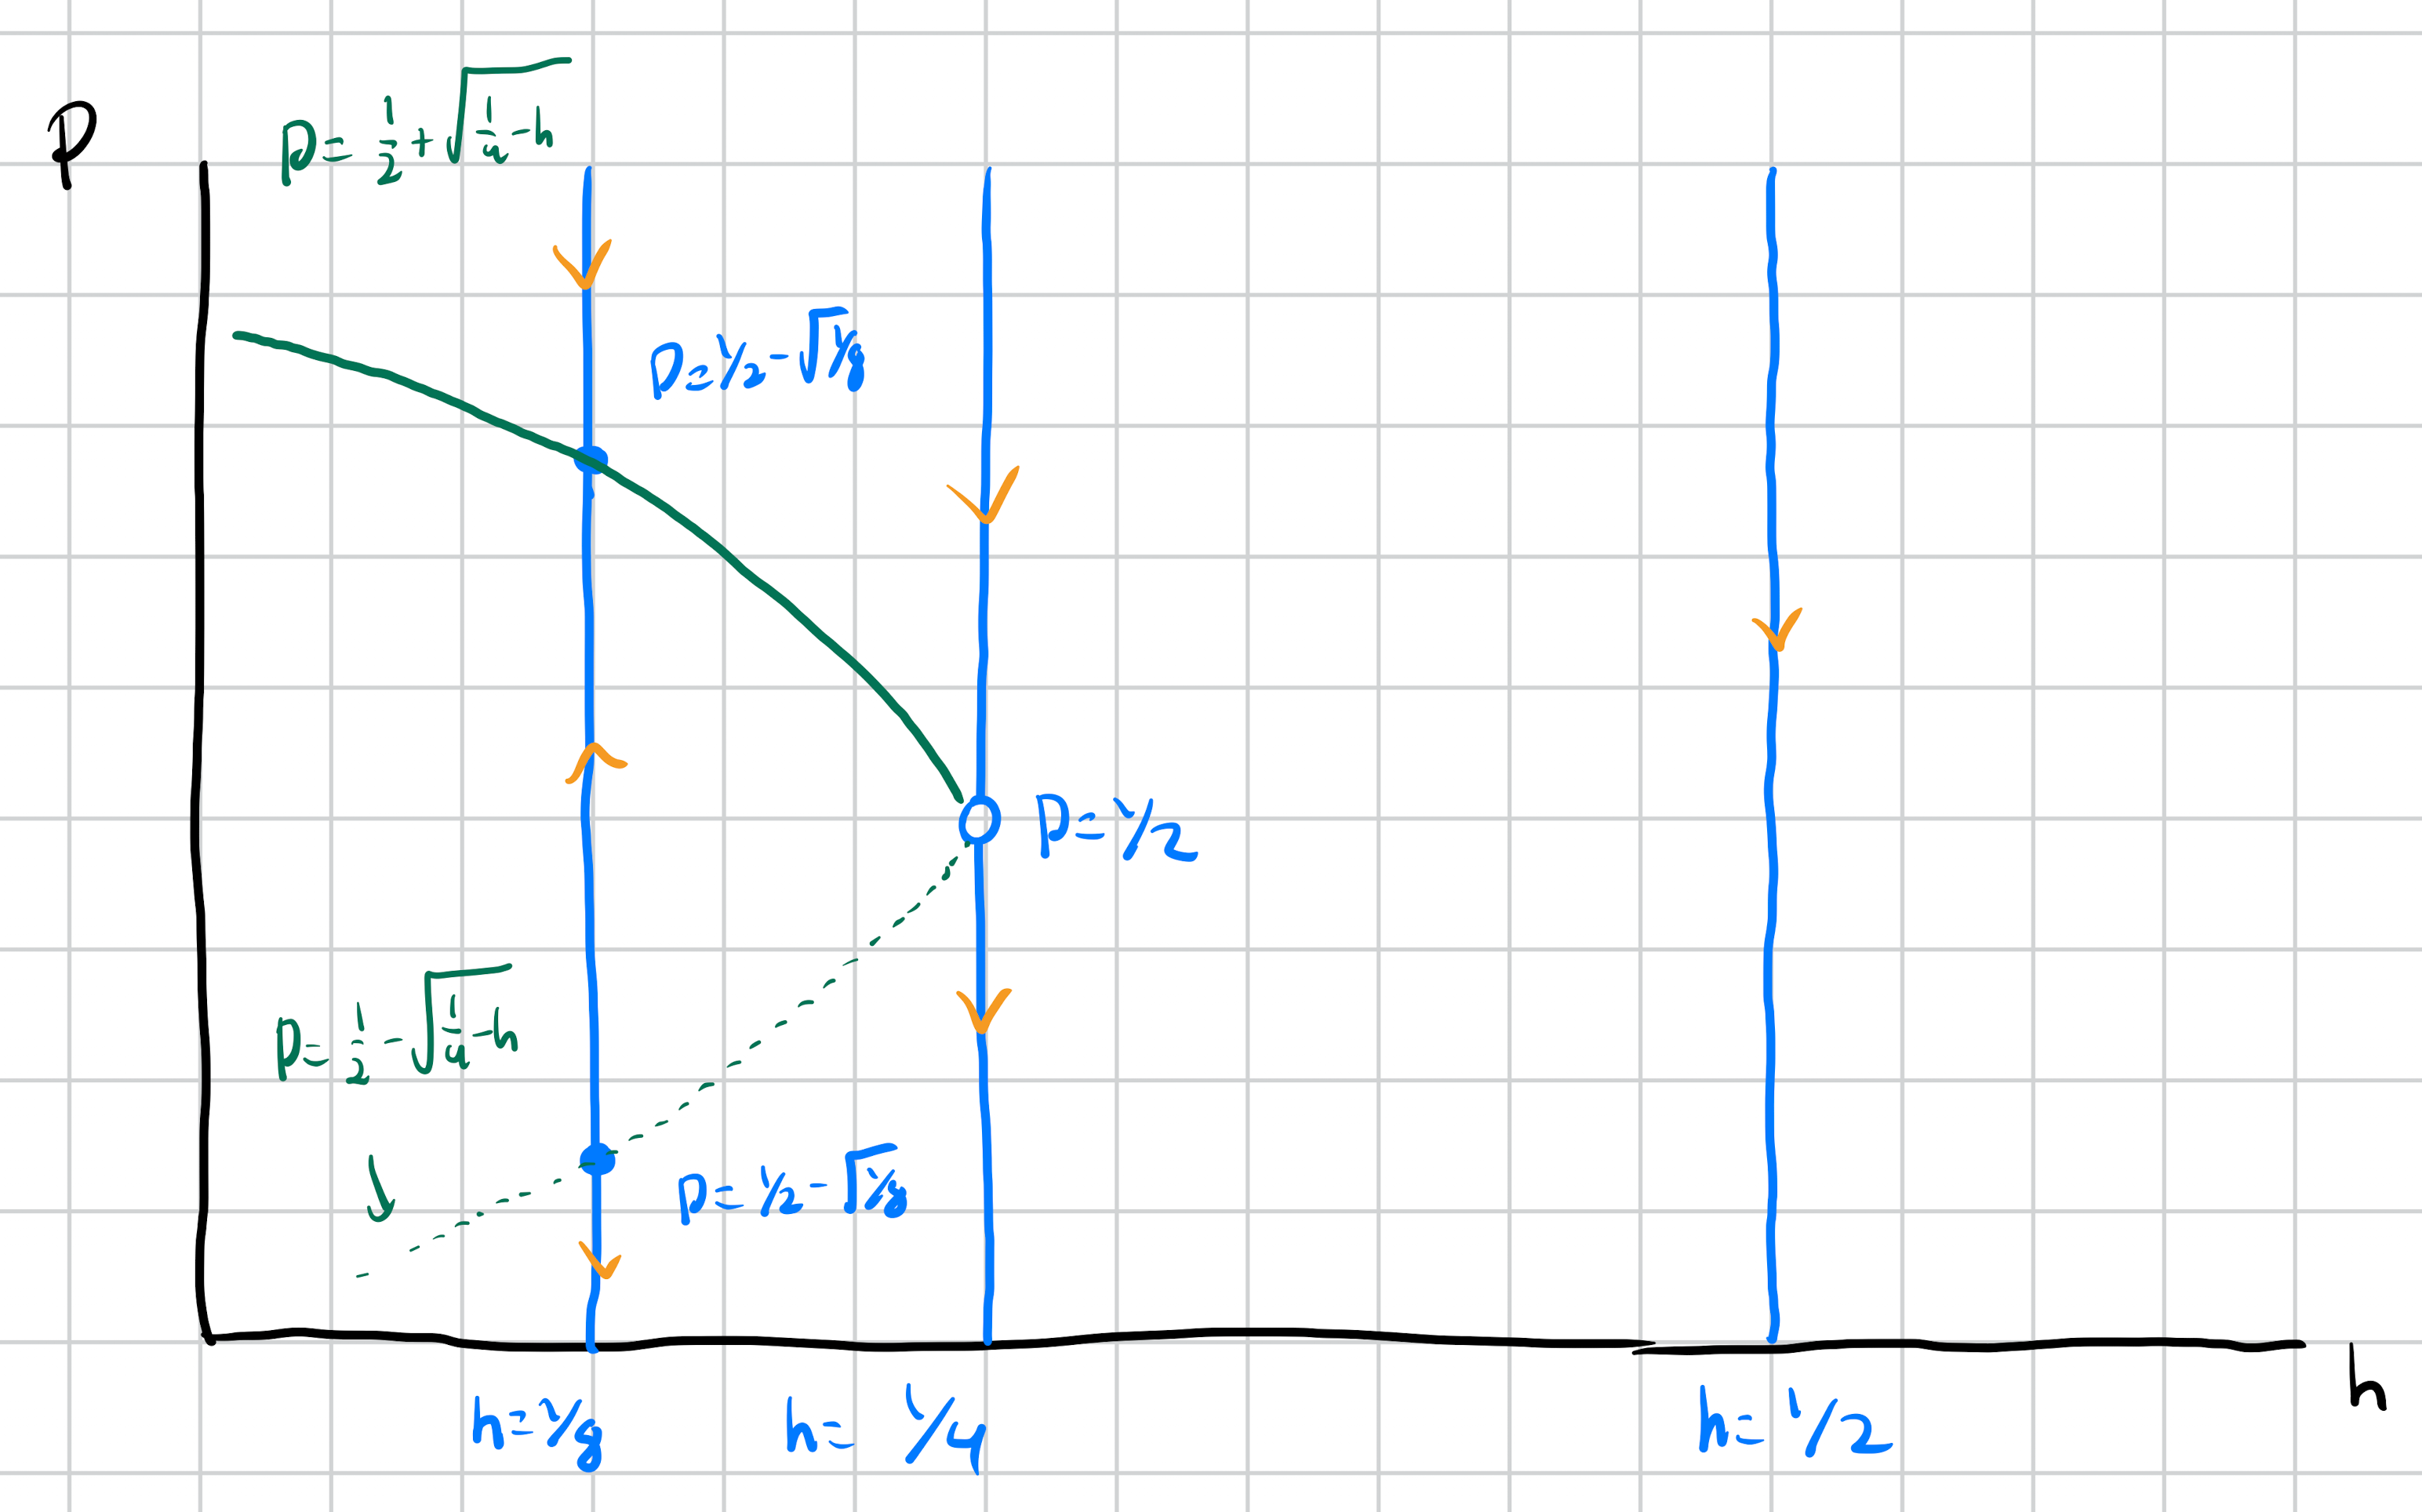
\includegraphics[width=12cm]{images/bifurcation_diagram_2.png}
  \end{center}
  \begin{itemize}
    \item If $h > 1/4$, the fish population will die out;
    \item If $h = 1/4$, the fish population will stabilize at $P = 1/2$;
    \item If $0 < h < 1/4$, the fish population will stabilize at a new, lower population.
  \end{itemize}
\end{example}
\begin{recall}
For
\begin{align*}
  \frac{dy}{dt} &= y^2 - c,
\end{align*}
there are three cases.
\begin{itemize}
  \item $c > 0$: two equilibrium solutions.
  \item $c = 0$: one equilibrium solution.
  \item $c < 0$: no equilibrium solutions.
\end{itemize}
When we graph $f$ against $y$, we see the following.
\begin{center}
  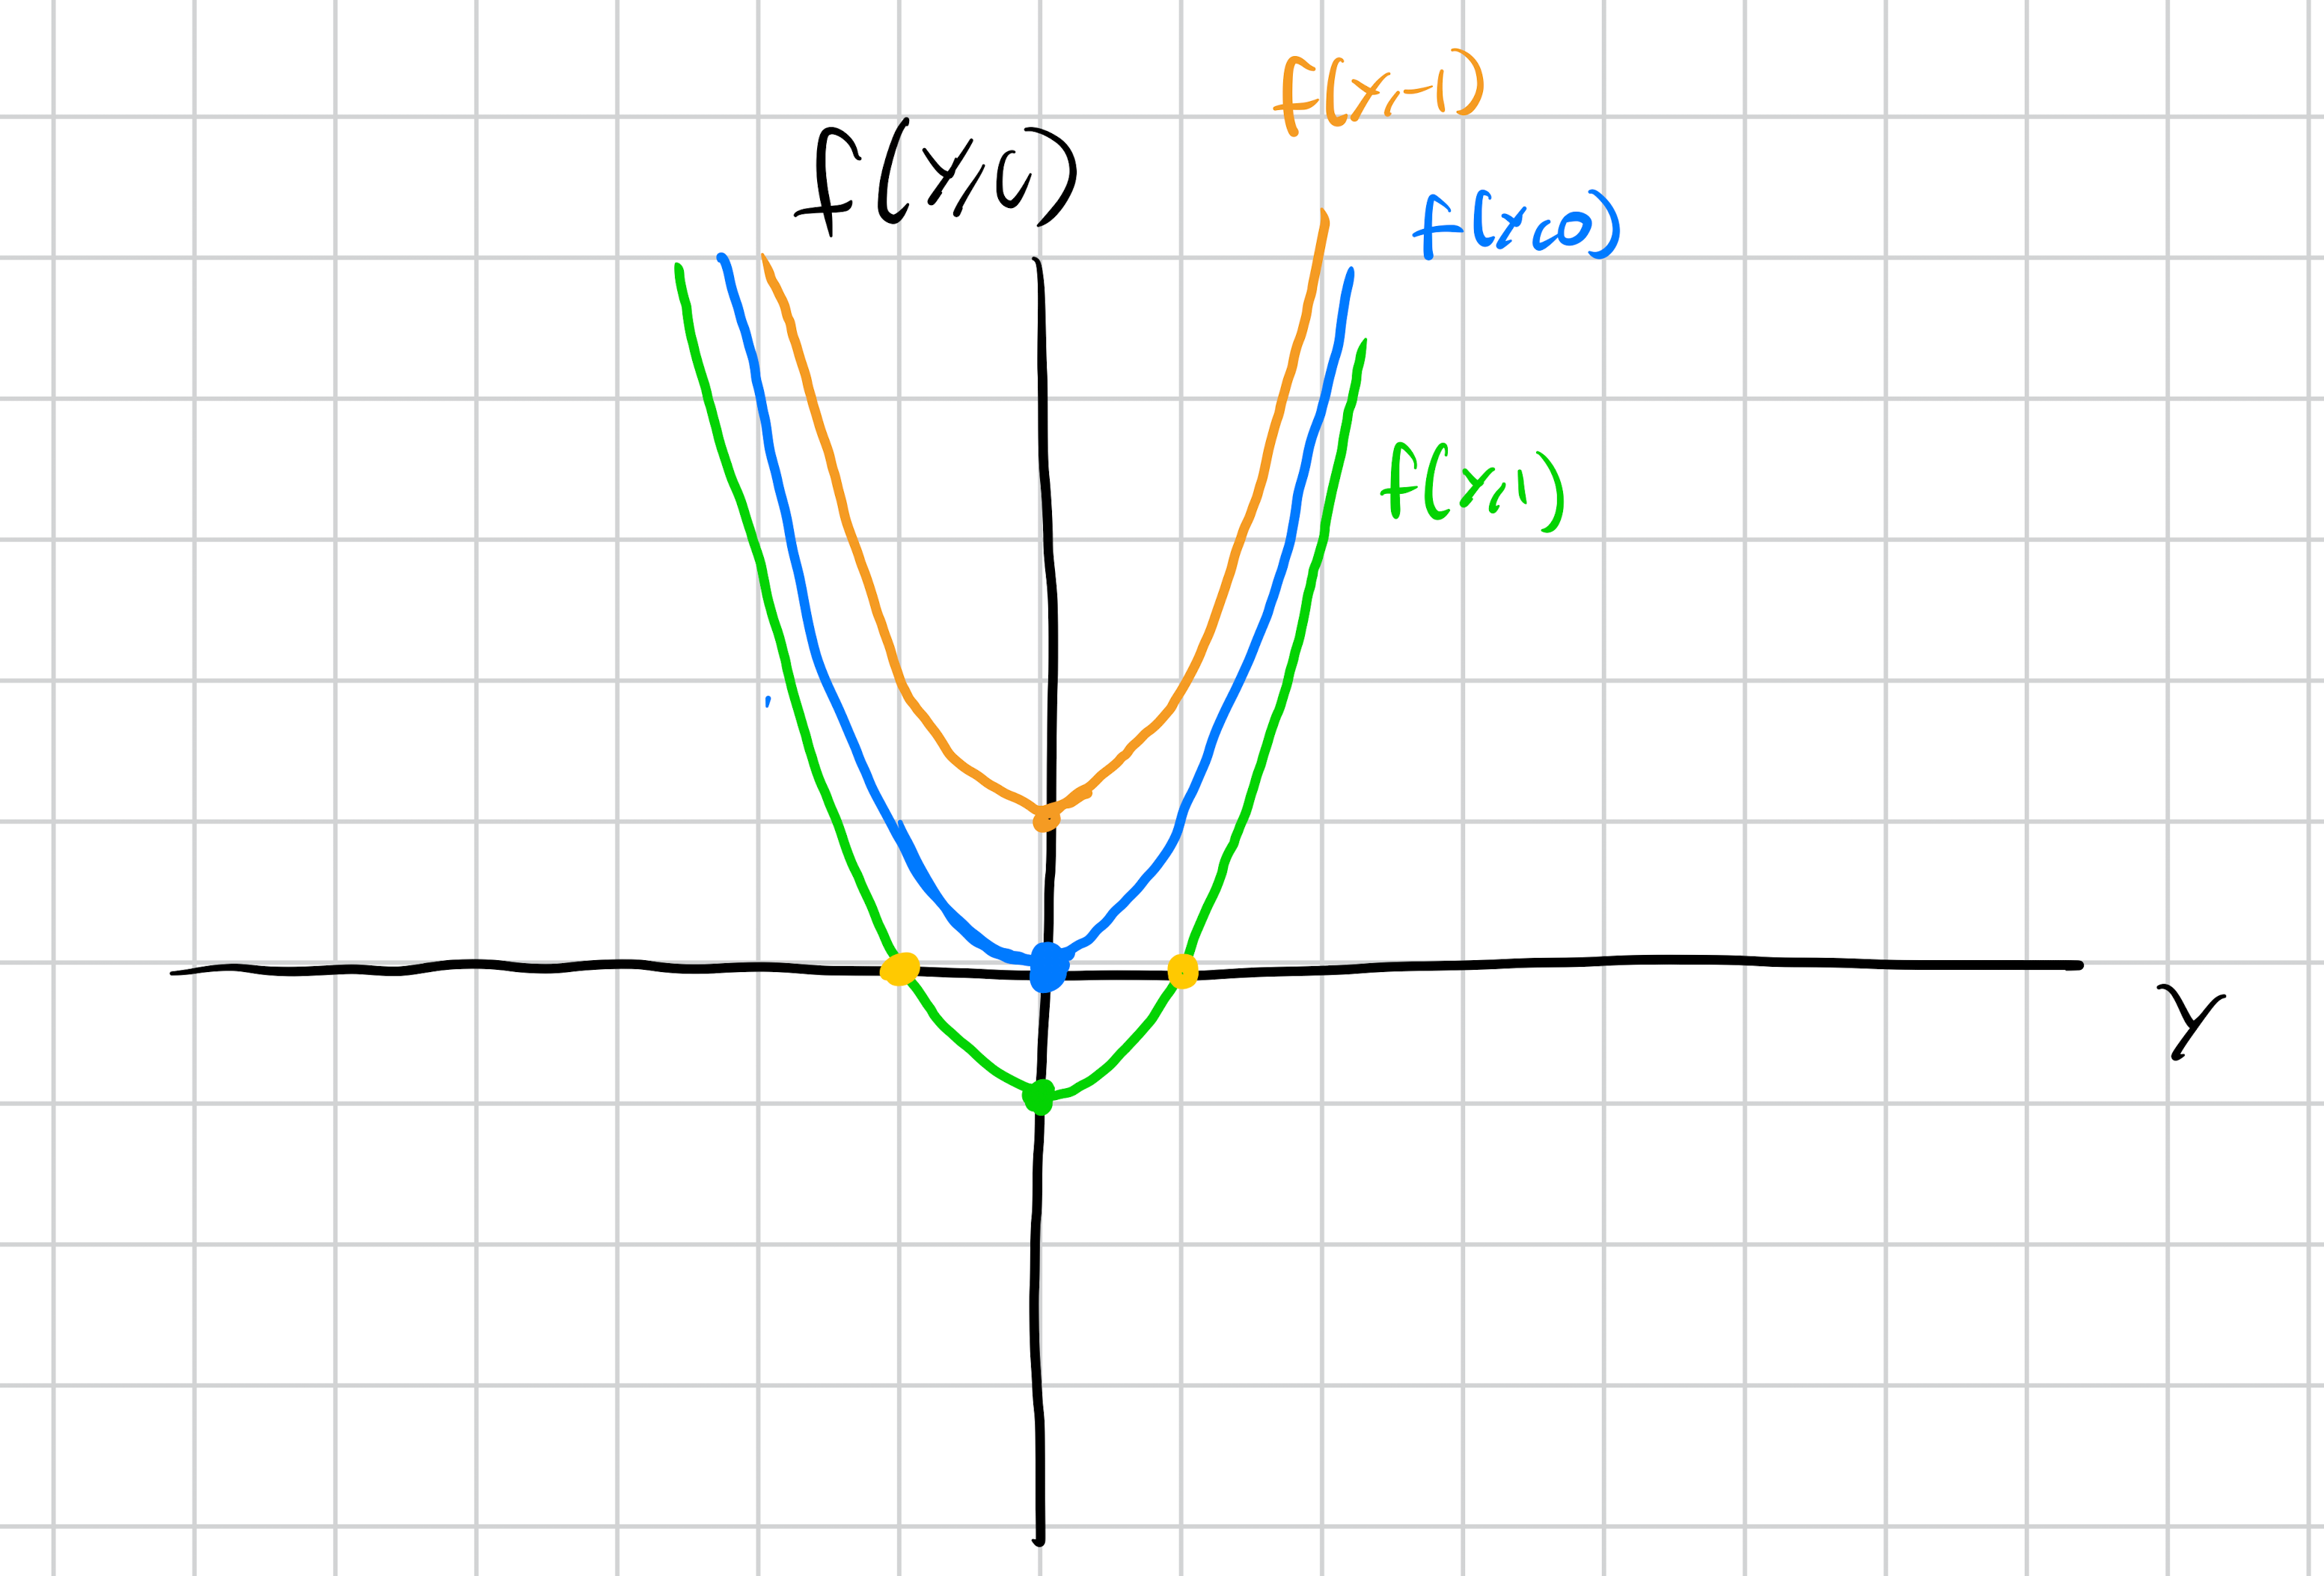
\includegraphics[width=7cm]{images/graph_to_bifurcation.png}
\end{center}
In particular, we can see that the bifurcation value occurs at $c = 0$, when the root of $f$ is tangent to the $y$ axis. This can be formalized in the following theorem.
\end{recall}
\begin{theorem}
  Let $y_0$ be an equilibrium solution. The point $c_0$ is a bifurcation value for the autonomous differential equation
  \begin{align*}
    \frac{dy}{dt} &= f(y,c)
  \end{align*}
  if and only if $f(y_0,c_0) = 0$ and $\frac{\partial f}{\partial y}\bigr\vert_{(y_0,c_0)} = 0$.
\end{theorem}
\subsection{First Order Linear Differential Equations}%
\begin{definition}
  A first-order differential equation of the form 
  \begin{align*}
    \frac{dy}{dt} &= a(t) y + b(t)\\
    \frac{dy}{dt} - a(t) y &= b(t)
  \end{align*}
  with $a(t),b(t)$ arbitrary functions of $t$ is known as a (first order) linear differential equation.
\end{definition}
\begin{example}\hfill
  \begin{enumerate}[(1)]
    \item $\frac{dy}{dt} +2y = e^{-t}$ is linear.
  \end{enumerate}
\end{example}
\begin{definition}[Homogeneous Linear Differential Equations]
  For
  \begin{align*}
    \frac{dy}{dt} - a(t) y &= b(t),
  \end{align*}
  if $b(t) = 0$ for all $t$, the linear differential equation is called homogeneous (or unforced). If $b(t)\neq 0$, we call this a non-homogeneous differential equation.
\end{definition}
\begin{definition}[Linearity Principle for Homogeneous Equations]
  Consider the homogeneous differential equation
  \begin{align*}
    \frac{dy}{dt} - a(t) y &= 0.
  \end{align*}
  \begin{enumerate}[(1)]
    \item If $y_h(t) $ is a solution of $ \frac{dy}{dt} - a(t) y = 0$, then $cy_h(t)$ is a solution for $\frac{dy}{dt} - a(t) y = 0$, for any $c\in \R$.
    \item If $y_1(t)$ and $y_2(t)$ are solutions of $\frac{dy}{dt} - a(t) y = 0$, then $\left(y_1 + y_2\right)(t)$ is a solution to $\frac{dy}{dt} - a(t) y = 0$.
  \end{enumerate}
\end{definition}
The proof of the linearity principle follows from the linearity of the derivative.
\begin{example}
  Let
  \begin{align*}
    \frac{dy}{dt} &= a(t) y + b(t).
  \end{align*}
  Note that the associated homogeneous differential equation is
  \begin{align*}
    \frac{dy}{dt} &= a(t) y.
  \end{align*}
  We can solve the associated homogeneous differential equation using separation of variables:
  \begin{align*}
    \frac{dy}{dt} &= a(t) y \\
    \int_{}^{} \frac{1}{y}\:dy &= \int_{}^{} a(t)\:dt\\
    \ln (y) &= \int_{}^{}a(t) dt + C\\
    y &= Ke^{\int_{}^{} a(t)\:dt}. \tag*{$C\in\R$}
  \end{align*}
  Note that the linearity principle does \textit{not} (necessarily) work for non-homogeneous differential equations.
\end{example}
\begin{example}[Failure of the Linearity Principle]
  Consider
  \begin{align*}
    \frac{dy}{dt} &= -y + 2. \tag*{(\textasteriskcentered)}
  \end{align*}
  Note that $b(t) = 2 \neq 0$.\newline

  One of the solutions to this equation is
  \begin{align*}
    y(t) = 2 - e^{-t}.
  \end{align*}
  We will show that $2y(t)$ is not a solution of (\textasteriskcentered).
  \begin{align*}
    \frac{d}{dt}\left(2\left(2-e^{-t}\right)\right)  &= 2e^{-t}\\
    -y(t) + 2 &= 2e^{-t} - 2.
  \end{align*}
\end{example}
\begin{theorem}[Extended Linearity Principle]
  Let
  \begin{align*}
    \diff{y}{t} &= a(t) y + b(t).\tag*{(\textasteriskcentered\textasteriskcentered)}
  \end{align*}
  \begin{enumerate}[(1)]
    \item If $y_h(t)$ is any solution of the homogeneous differential equation
      \begin{align*}
        \diff{y}{t} &= a(t) y,
      \end{align*}
      and $y_p(t)$ is any solution of (\textasteriskcentered\textasteriskcentered). Then, $y_h(t) + y_p(t)$ is a solution to (\textasteriskcentered\textasteriskcentered).
    \item If $y_1(t)$ and $y_2(t)$ are solutions to (\textasteriskcentered\textasteriskcentered), $y_1(t) - y_2(t)$ provides a solution to the homogeneous differential equation
      \begin{align*}
        \diff{y}{t} &= a(t) y.
      \end{align*}
  \end{enumerate}
\end{theorem}
\begin{proof}\hfill
  \begin{enumerate}[(1)]
    \item 
      \begin{align*}
        \frac{d}{dt}\left(y_h(t) + y_p(t)\right) &= \frac{d}{dt}\left(y_h(t)\right) + \diff{}{t}\left(y_p(t)\right)\\
                                                 &= a(t)y_h(t) + a(t)y_p(t) + b(t)\\
                                                 &= a(t)\left(y_h(t) + y_p(t)\right) + b(t).
      \end{align*}
    \item 
      \begin{align*}
        \frac{d}{dt}\left(y_1(t) - y_2(t)\right) &= \frac{d}{dt}\left(y_1(t)\right) - \diff{}{t}\left(y_2(t)\right)\\
                                                 &= \left(a(t)y_1(t) + b(t)\right) - \left(a(t)y_2(t) - b(t)\right)\\
                                                 &= a(t)\left(y_1(t)-y_2(t)\right).
      \end{align*}
  \end{enumerate}
\end{proof}
Note that, as a result of the extended linearity principle, all solutions to a non-homogeneous first-order linear equation are of the form $y(t) = cy_h(t) + y_{p}(t)$, where $y_{p}(t)$ is \textit{any} solution to the equation.
\begin{example}
  Let
  \begin{align*}
    \diff{y}{t} &= -2y + e^{t}.
  \end{align*}
  We can see that $b(t) = e^{t}$, and the general solution to $\diff{y}{t} = -2y$ is $Ke^{-2t}$ for $K\in \R$.\newline

  Now, we look at
  \begin{align*}
    \frac{dy}{dt} + 2y &= e^{t}
  \end{align*}
  We make a guess that
  \begin{align*}
    y_p(t) &= \alpha e^{t}.
  \end{align*}
  Then,
  \begin{align*}
    \diff{y}{t} + 2y &= \alpha e^{t} + 2\alpha e^{t}\\
                     &= e^{t}.
  \end{align*}
  Thus, $\alpha = \frac{1}{3}$, implying that $y_p(t) = \frac{1}{3}e^{t}$.\newline

  Thus, the general solution is
  \begin{align*}
    y(t) &= \frac{1}{3}e^{t} + Ke^{-2t}.
  \end{align*}
\end{example}
\begin{example}
  Let's try to find the general solution to 
  \begin{align*}
    \diff{y}{t} &= -2y + \cos(3t).
  \end{align*}
  We are aware of the general solution of the homogeneous equation $\frac{dy}{dt} = -2y$, which is $y_h(t) = Ke^{-2t}$.\newline

  Now, we look at
  \begin{align*}
    \diff{y}{t} + 2y &= \cos(3t)
  \end{align*}
  to find a particular solution. We take a guess of $y_p(t) = A\cos(3t) + B\sin(3t)$. Then,
  \begin{align*}
    \diff{y}{t} + 2y &= \left(-3A + 2B\right)\sin(3t) + \left(2A + 3B\right)\cos(3t).
  \end{align*}
  Thus, $3A = 2B$ and $2A + 3B = 1$, yielding $B = \frac{3}{13}$ and $A = \frac{2}{13}$.\newline

  Therefore, the general solution is
  \begin{align*}
    y(t) &= \frac{2}{13}\cos(3t) + \frac{3}{13}\sin(3t) + Ke^{-2t}.
  \end{align*}
\end{example}
\begin{center}
  \renewcommand{\arraystretch}{1.5}
  \begin{tabular}{c|c}
    $b(t)$ & Guess for $y_p(t)$\\
    \hline
    $ae^{\alpha t}$ & $Ae^{\alpha t}$\\
    $a\cos\left(\beta t\right)$ & $A\cos\left(\beta t\right) + B\cos\left(\beta t\right)$\\
    $a\sin\left(\beta t\right)$ & $A\cos\left(\beta t\right) + B\cos\left(\beta t\right)$\\
    $a\cos\left(\beta t\right) + b\sin\left(\beta t\right)$ & $A\cos\left(\beta t\right) + B\cos\left(\beta t\right)$\\
    $n$-th degree polynomial & $A_nt^{n} + A_{n-1}t^{n-1} + \cdots + A_1t + A_0$
  \end{tabular}
\end{center}
\subsection{Integrating Factors}%
We can formalize the aforementioned ``lucky guess'' method by creating an integrating factor.
\begin{derivation}[Integrating Factor]
  Consider the equation
  Consider a factor $\mu(t)$.
  \begin{align*}
    \diff{y}{t} &= a(t) y + b(t)\\
    \diff{y}{t} - a(t) y &= b(t)\\
    \diff{y}{t} + g(t) y &= b(t),
  \end{align*}
  where we define $g(t) = -a(t)$. We multiply each side of this differential equation by $\mu(t)$, yielding
  \begin{align*}
    \mu(t)\left(\diff{y}{t} + g(t)y\right) &= \mu(t)b(t)\\
    \mu(t)\diff{y}{t} + \mu(t)g(t)y &= \mu(t)b(t).
  \end{align*}
  Examining the left-hand side, it would be very convenient if $\diff{\left(\mu(t)y(t)\right)}{t} = \mu(t)\diff{y}{t} + y(t)\diff{\mu}{t}$. Then, we would have
  \begin{align*}
    \diff{}{t}\left(\mu(t)y(t)\right) &= \mu(t)b(t),
  \end{align*}
  where $\diff{\mu}{t} = \mu(t)g(t)$. Then,
  \begin{align*}
    \mu(t)y(t) &= \int_{}^{} \mu(t)b(t)\:dt\\
    y(t) &= \frac{1}{\mu(t)}\int_{}^{} \mu(t)b(t)\:dt.
  \end{align*}
  Orienting our focus to the condition of $\diff{\mu}{t} = \mu(t)g(t)$, we solve for $\mu$ by separation of variables.
  \begin{align*}
    \diff{\mu}{t} &= \mu g(t)\\
    \int_{}^{} \frac{1}{\mu}\:d\mu &= \int_{}^{} g(t)\:dt\\
    \ln \left\vert \mu \right\vert &= \int_{}^{} g(t)\:dt\\
    \left\vert \mu \right\vert &= e^{C + \int_{}^{} g(t)\:dt}\\
    \mu &= K e^{\int_{}^{} g(t)\:dt}.
  \end{align*}
\end{derivation}
\begin{definition}[Integrating Factor]
  For a non-homogeneous linear differential equation,
  \begin{align*}
    \diff{y}{t} + g(t)y &= b(t)
  \end{align*}
  the integrating factor is a family of functions such that
  \begin{align*}
    \mu(t) &= Ke^{\int_{}^{} g(t)\:dt}.
  \end{align*}
  In particular, we can let $K = 1$, yielding the factor
  \begin{align*}
    \mu(t) &= e^{\int_{}^{} g(t)\:dt}.
  \end{align*}
\end{definition}
\begin{example}
  We wish to solve
  \begin{align*}
    x\diff{y}{x} - 4y &= x^{6}e^{x}.
  \end{align*}
  First, we divide out $x$, yielding
  \begin{align*}
    \diff{y}{x} - \frac{4}{x}y &= x^5 e^x.
  \end{align*}
  Now, we find the integrating factor,
  \begin{align*}
    \mu(x) &= e^{\int_{}^{} -\frac{4}{x}\:dx}\\
           &= e^{-4\ln |x|}\\
           &= e^{\ln\left\vert x^{-4}\right\vert}\\
           &= e^{\ln\left\vert x^{-4} \right\vert}
           &= \frac{1}{x^4}.
  \end{align*}
  Multiplying through, we get
  \begin{align*}
    x^{-4}\diff{y}{x} - 4x^{-5}y &= xe^{x}\\
    \diff{}{x}\left(x^{-4} y\right) &= xe^{x}\\
    x^{-4} y &= \int_{}^{} xe^{x}\:dx\\
    y &= x^{4}\left(xe^{x} - e^{x} + C\right)\\
      &= \underbrace{x^{5}e^{x} - x^4e^{x}}_{y_p(x)} + \underbrace{Cx^{4}}_{y_h(x)}.
  \end{align*}
\end{example}
\begin{example}
  Consider the equation
  \begin{align*}
    \diff{y}{t} + y &= 17\sin(4t).
  \end{align*}
  The coefficient in front of $y$ is $1$, so our integrating factor is
  \begin{align*}
    \mu(t) &= e^{\int_{}^{} \:dt}\\
           &= e^{t}.
  \end{align*}
  Multiplying through, we get
  \begin{align*}
    \diff{}{t}\left(e^{t} y\right) &= 17e^{t}\sin(4t)\\
    e^{t} y &= \int_{}^{} 17e^{t}\sin(4t)\:dt\\
            &= 17\int_{}^{} e^{t}\sin(4t)\:dt\\
            &= e^{t}\sin(4t) - 4e^{t}\cos(4t)+ C\tag*{Integration by Parts.}\\
    y &= \underbrace{\sin(4t) - 4\cos(4t)}_{y_p(t)} + \underbrace{Ce^{-4t}}_{y_h(t)}.
  \end{align*}
  Alternatively, we can solve this equation using a ``lucky guess'' method. Starting with the homogeneous equation, we find
  \begin{align*}
    \diff{y}{t} + y &=0 \\
    \int_{}^{} \frac{1}{y}\:dy &= \int_{}^{} -1\:dt\\
    \ln \left\vert y \right\vert &= -t + C\\
    y_h &= Ce^{-t}.
  \end{align*}
  Now, looking at the non-homogeneous equation, we look at
  \begin{align*}
    \diff{y}{t} + y &= 17 \sin(4t).
  \end{align*}
  The lucky guess we take is $y_p(t) = A\sin(4t) + B\cos(4t)$, yielding
  \begin{align*}
    \diff{y_p}{t} + y &= 17\sin(4t)\\
    4A\cos(4t) - 4B\sin(4t) + \left(A \sin(4t) + B\cos(4t)\right) &= 17\sin(4t)\\
    (4A + B)\cos(4t) + \left(A - 4B\right)\sin(4t) &= 17\sin(4t).
  \end{align*}
  The system of equations yields $4A + B = 0$ and $A - 4B = 17$, meaning $A = 1$ and $B = -4$. Thus, $y_p(t)$ is
  \begin{align*}
    y_p(t) &= \cos(4t) - 4\sin(4t).
  \end{align*}
  Our general solution is, finally,
  \begin{align*}
    y(t) &= \cos(4t) - 4\sin(4t) + Ce^{-t}.
  \end{align*}
\end{example}
\section{Systems of First-Order Differential Equations}%
\subsection{Modeling with Systems}%
Consider a second-order differential equation
\begin{align*}
  y'' + 2y' + 3y + 5 = 0.
\end{align*}
In order to solve these, we need to start by passing our second order differential equation into a system of first-order differential equations.
\begin{definition}[System of Differential Equations]
  A pair of differential equations of the form
  \begin{align*}
    \frac{dx}{dt} &= f_2\left(x,y,2\right)\\
    \frac{dy}{dt} &= f_1\left(x,y,t\right)
  \end{align*}
  where $f_1$ and $f_2$ are functions of $x,y,t$ defined on a common set $S$ is called a system of two first-order differential equations.
\end{definition}
\begin{definition}[Linear System of Differential Equations]
  The system of two first order differential equations is linear if $f_1(x,y,t)$ and $f_2(x,y,t)$ are linear in $x$ and $y$.
\end{definition}
\begin{example}
  If
  \begin{align*}
    \diff{x}{t} &= a_1(t)x + a_2(t)y + a_3(t)\\
    \diff{y}{t} &= b_1(t)x + b_2(t)y + b_3(t)
  \end{align*}
\end{example}
\begin{example}[Passing Second-Order Equation into System of First-Order Equations]
  Let
  \begin{align*}
    2y'' - 5y' + y &= 0.
  \end{align*}
  To solve this equation, we define
  \begin{align*}
    x_1 &= y\\
    x_2 &= y'.
  \end{align*}
  Taking derivatives, we get
  \begin{align*}
    x_1' &= y'\\
    x_2' &= y''.
  \end{align*}
  Substituting, we get
  \begin{align*}
    x_1' &= x_2\\
    x_2' &= \frac{5}{2}x_2 - \frac{1}{2}x_1.
  \end{align*}
\end{example}
\begin{example}[Passing Third-Order Differential Equation into System of First-Order Equations]
  Let
  \begin{align*}
    y''' + 3y'' + 2y' - 5y = \sin(2t)
  \end{align*}
  Let
  \begin{align*}
    x_1 &= y\\
    x_2 &= y'\\
    x_3 &= y''.
  \end{align*}
  In general, when creating our system, we stop one derivative short of the order of the equation. Taking derivatives, we get
  \begin{align*}
    x_1' &= y'\\
    x_2' &= y''\\
    x_3' &= y''',
  \end{align*}
  and substituting, we get
  \begin{align*}
    x_1' &= x_2\\
    x_2' &= x_3\\
    x_3' &= -3x_3'' - 2x_2' + 5x_1 + \sin(2t).
  \end{align*}
\end{example}
\begin{definition}[Essentials for a System]
  Let
  \begin{align*}
    \diff{R}{t} &= \underbrace{aR - bRF}_{f_1(R,F)}\\
    \diff{F}{t} &= \underbrace{cRF - dF}_{f_2(R,F)},
  \end{align*}
  where $a,b,c,d > 0$ are positive constants.\footnote{This is known as the Lotka--Volterra model.}
  \begin{itemize}
    \item The equilibrium solutions are a pair of constant functions $R(t)$ and $F(t)$ that solve the system, or for which $f_1(R(t),F(t))$ and $f_2(R(t),F(t))$ are simultaneously equal to zero.
    \item A general solution to the system is a pair of functions $R(t)$ and $F(t)$ that, taken together, satisfy the system of equations.
    \item As $t$ varies, the pair $\left(R(t),F(t)\right)$ traces out the \textit{solution curve} in the $RF$-plane. Its size and shape are determined by the initial condition, $\left(R(0),F(0)\right)$.
    \item The phase plane for the system of differential equations is the $RF$-plane in which the vector 
      \begin{align*}
        \mathbf{V} &= R'(t)\hat{i} + F'(t)\hat{j}\\
                   &= f_1\left(R,F\right)\hat{i} + f_2\left(R,F\right)\hat{j}
      \end{align*}
      is drawn at a grid of points $\left(R_i,F_i\right)$.
    \item A phase portrait is the phase plane with enough solution curves to show how the solutions behave in every part of the plane.
  \end{itemize}
\end{definition}
\begin{example}[Solutions for a System of Differential Equations]
Consider the following Lotka--Volterra model.
\begin{align*}
  \diff{R}{t} &= 2R - 1.2RF\\
  \diff{F}{t} &= -F + 0.9RF.
\end{align*}
We start with the equilibrium points.
\begin{align*}
  \diff{R}{t} &= 0\\
  0 &= R\left(2 - 1.2F\right),\\
  R &= 0
  F &= \frac{2}{1.2}\\
  \diff{F}{t} &= 0\\
  0 &= -F + 0.9RF\\
  \intertext{When $R = 0$}
  -F &= 0\\
  F &= 0.\\
  \intertext{When $F = \frac{2}{1.2}$}
  0 &= F\left(0.9R - 1\right)\\
  R &= \frac{1}{0.9}.
\end{align*}
Thus, the equilibrium solutions are at $\left(\frac{1}{0.9},\frac{2}{1.2}\right)$ and at $\left(0,0\right)$. We can see that the phase portrait seems to approach a fixed point towards the point $\left(1.11,1.67\right)$.
\begin{center}
  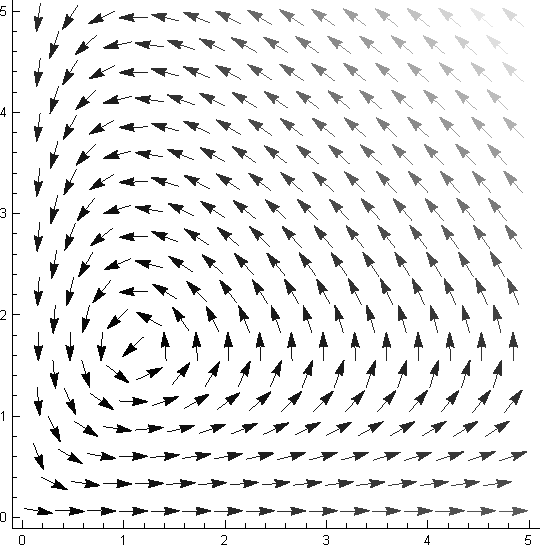
\includegraphics[width=10cm]{images/lv_eqns_1.pdf}
\end{center}
If we take the initial condition of $R(0) = 1$ and $F(0) = 1$, and send $F$ to $0$, we see that $R$ tends toward infinity.\newline

Meanwhile, if we send $R$ to $0$, we see that the number of tends to $0$.\newline

Using a computer, we can plot the solution to these initial conditions as seen below.
\begin{center}
  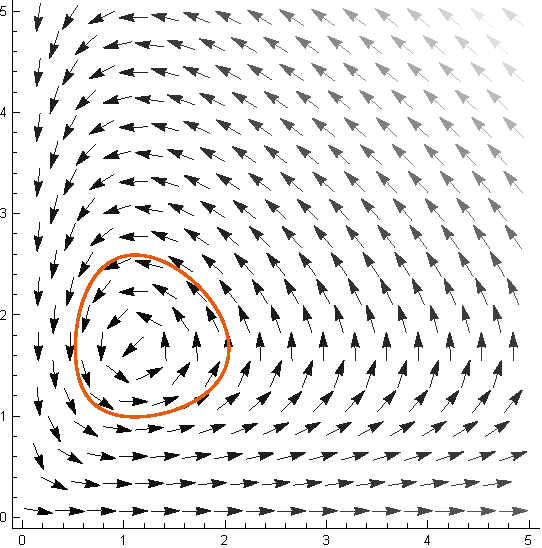
\includegraphics[width=10cm]{images/lv_eqns_w_sol.pdf}
\end{center}
As we send the initial conditions closer to $(1.11,1.67)$, we see that the solution curves seem to approach an equilibrium value.
\begin{center}
  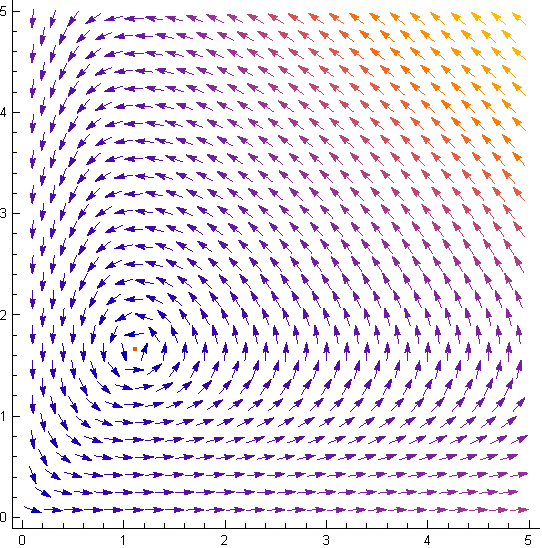
\includegraphics[width=10cm]{images/lv_eqns_w_sol_2.pdf}
\end{center}
\end{example}
\begin{example}[An Alternative Lotka--Volterra Model]
  Consider the following altered model.
\begin{align*}
  \diff{R}{t} &= 2R\left(1 - \frac{R}{2}\right) - 1.2RF\\
  \diff{F}{t} &= -F + 0.9RF.
\end{align*}
Note that, with this new initial condition, we see that the solution approaches an equilibrium point.
\begin{center}
  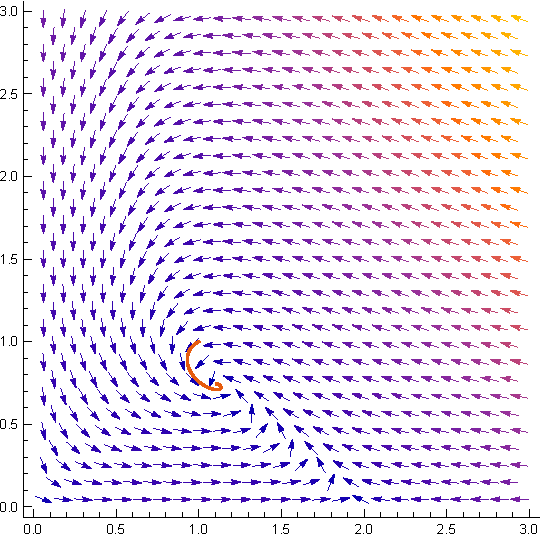
\includegraphics[width=10cm]{images/modified_lv_eqns_w_sol.pdf}
\end{center}
Solving for the equilibrium solutions, we get $R = F = 0$, $R = 2, F = 0$, and $R = \frac{1}{0.9},F = 0.74$.\newline

In particular, with this modified equation, we can see that as $F$ tends to $0$, the number of rabbits approaches a stable equilibrium of $R = 2$ as $t\rightarrow\infty$. Meanwhile, if $R$ tends to $0$, then $F$ also tends to $0$.\newline

In general, this modified Lotka--Volterra model approaches some equilibrium point regardless of the starting condition, which differs greatly to the periodic solutions that were found in the original model.
\end{example}
\subsection{Representing Systems of Equations with Vector Fields}%
Consider the system of differential equations,
\begin{align*}
  \diff{x}{t} &= f(x,y)\\
  \diff{y}{t} &= g(x,y).
\end{align*}
Note that this system is autonomous. We let
\begin{align*}
  \vec{Y}(t) &= \begin{pmatrix}x(t)\\y(t)\end{pmatrix}\\
  \vec{F}(x,y) &= \begin{pmatrix}f(x,y)\\g(x,y)\end{pmatrix}.
\end{align*}
We can see that
\begin{align*}
  \diff{\vec{Y}}{t} &= \begin{pmatrix}\diff{x}{t}\\\diff{y}{t}\end{pmatrix}\\
                    &= \begin{pmatrix}f(x,y)\\g(x,y)\end{pmatrix}\\
                    &= \vec{F}(x,y).
\end{align*}
\begin{definition}
  An equilibrium point $\vec{Y}_0$ of the system $\diff{\vec{Y}}{t} = \vec{F}\left(\vec{Y}\right)$ is a point a which $\vec{F}\left(\vec{Y}\right) = \vec{0}$.
\end{definition}
\begin{example}
  Consider the system
  \begin{align*}
    \diff{x}{t} &= x\\
    \diff{y}{t} &= y.
  \end{align*}
  The corresponding vector field $\vec{Y}$ is
  \begin{align*}
    \vec{Y} &= \begin{pmatrix}x\\y\end{pmatrix},
  \end{align*}
  which has the following vector field.
  \begin{center}
    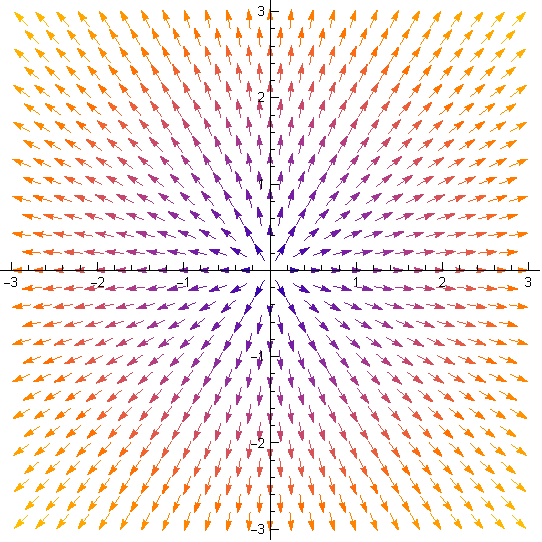
\includegraphics[width=5cm]{images/example_vector_field.pdf}
  \end{center}
  The direction field is the depiction of the vector field with where all vectors are of unit length.\newline

  Meanwhile, if we have the system
  \begin{align*}
    \diff{x}{t} &= y\\
    \diff{y}{t} &= -x,
  \end{align*}
  the direction field looks as follows.
  \begin{center}
    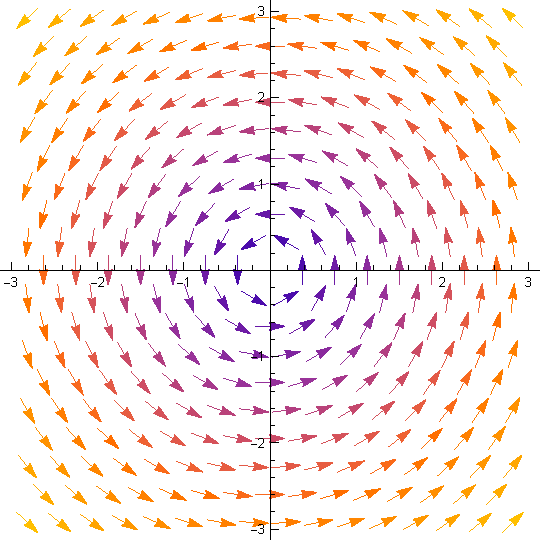
\includegraphics[width=7cm]{images/example_vector_field_2.pdf}
  \end{center}
  We can verify that 
  \begin{align*}
    \vec{y}(t) &= \begin{pmatrix}\cos(t)\\-\sin(t)\end{pmatrix}
  \end{align*}
  is a solution by plugging it into the expression for $\diff{\vec{y}}{t}$.
\end{example}
\begin{definition}[Decoupled System]
  A system of linear equations of the form
  \begin{align*}
    \diff{x}{t} &= f(x)\\
    \diff{y}{t} &= f(y)
  \end{align*}
   is known as a completely decoupled system.
\end{definition}
\begin{example}
  Considering the system
  \begin{align*}
    \diff{x}{t} &= -2x\\
    \diff{y}{t} &= -y,
  \end{align*}
  we can solve to get
  \begin{align*}
    x(t) &= k_1e^{-2t}\\
    y(t) &= k_2e^{-t}.
  \end{align*}
  Thus, the general solution to the system is of the form
  \begin{align*}
    \vec{F}(t) &= \begin{pmatrix}k_1e^{-2t}\\k_2e^{-t}\end{pmatrix}.
  \end{align*}
  Consider the IVP with 
  \begin{align*}
    \vec{Y}(0) &= \begin{pmatrix}1\\1\end{pmatrix}.
  \end{align*}
  Then, we get
  \begin{align*}
    k_1 &= 1\\
    k_2 &= 1,
  \end{align*}
  meaning the solution to the particular IVP is
  \begin{align*}
    \vec{F}(t) &= \begin{pmatrix}e^{-2t}\\e^{-t}\end{pmatrix}.
  \end{align*}
  Note that we can write a closed form function, $x = y^2$, which allows us to draw a solution curve on the phase plane.
\end{example}
\begin{example}[A Partially Decoupled System]
Consider the system
\begin{align*}
  \diff{x}{t} &= 3x + 2y\\
  \diff{y}{t} &= -y.
\end{align*}
Since $\diff{x}{t}$ depends on both $x$ and $y$, but $\diff{y}{t}$ depends only on $y$, we can solve for $y$ independent of $x$, and substitute.
\begin{align*}
  y(t) &= k_2e^{-t}
\end{align*}
Substituting, we have
\begin{align*}
  \diff{x}{t} - 3x &= 2k_2e^{-t}.
\end{align*}
Using the integrating factor $\mu(t) = e^{-3t}$, we have
\begin{align*}
  e^{-3t}\diff{x}{t} - 3xe^{-3t} &= 2k_2e^{-4t}\\
  \diff{}{t}\left(xe^{-3t}\right) &= 2k_2e^{-4t}\\
  xe^{-3t} &= -\frac{1}{2}k_2e^{-4t} + C\\
  x &= -\frac{1}{2}k_2e^{-t} + k_1e^{3t}.
\end{align*}
Thus, we have
\begin{align*}
  \vec{F}(t) &= \begin{pmatrix}-\frac{1}{2}k_2e^{-t} + k_1e^{3t} \\ k_2e^{-t}\end{pmatrix}.
\end{align*}
Consider the initial condition
\begin{align*}
  \vec{Y}(0) &= \begin{pmatrix}1 \\ 0\end{pmatrix}
\end{align*}
Then, substituting into our equation, we get $k_2 = 0$, $k_1 = 1$, so our solution is
\begin{align*}
  \vec{F}(t) &= \begin{pmatrix}e^{3t}\\0\end{pmatrix}.
\end{align*}
\end{example}
\subsection{Euler's Method for Systems of Differential Equations}%
Consider a first order autonomous system
\begin{align*}
\diff{x}{t} &= f(x,y)\\
\diff{y}{t} &= g(x,y),
\end{align*}
with $x(0) = x_0$ and $y(0) = y_0$.\newline

To approximate this solution, we can use the phase diagram. Converting to vector notation, we have
\begin{align*}
  \vec{F}(x,y) &= \begin{pmatrix}f(x,y)\\g(x,y)\end{pmatrix}\\
  \diff{\vec{Y}}{t} &= \vec{F}\left(\vec{Y}\right).
\end{align*}
Starting from $\left(x_0,y_0\right)$ in the phase diagram, we get the first step, $\left(x_1,y_1\right) = \left(x_0 ,y_0\right) + \left(\delta t\right) \vec{F}\left(x_0,y_0\right)$. Similarly, we inductively find
\begin{align*}
  \left(x_{k+1},y_{k+1}\right) &= \left(x_k,y_k\right) + \delta t \vec{F}\left(x_k,y_k\right).
\end{align*}
Componentwise, we have
\begin{align*}
  x_{k+1} &= x_k + \left(\delta t\right)f\left(x_k,y_k\right)\\
  y_{k+1} &= y_k + \left(\delta t\right) g\left(x_k,y_k\right).
\end{align*}
\begin{example}
  Consider the system
  \begin{align*}
    \diff{x}{t} &= -y\\
    \diff{y}{t} &= x-y
  \end{align*}
  with the initial condition 
  \begin{align*}
    \vec{Y}(0) &= \begin{pmatrix}1\\1\end{pmatrix},
  \end{align*}
  and step size $\delta t = 0.25$. We hope to approximate the solution at $t = 0.5$.
  \begin{center}
    \begin{tabular}{c|c|c|c|c|c}
      $k$ & $t_k$ & $x_k$ & $y_k$ & $f\left(x_k,y_k\right)$ & $g\left(x_k,y_k\right)$\\
      \hline
      $0$ & $0$ & $1$ & $1$ & $-1$ & $0$\\
      $1$ & $0.25$ & $0.75$ & $1$ & $-1$ & $-0.25$\\
      $2$ & $0.5$ & $0.5$ & $0.9375$ & --- & ---
    \end{tabular}
  \end{center}
\end{example}
\begin{example}
  Consider the Lotka--Volterra model
  \begin{align*}
    \diff{R}{t} &= 2R - 1.2RF\\
    \diff{F}{t} &= -F + 0.9RF
  \end{align*}
  with initial condition $R(0) = 1$ and $F(0) = 1$. Using Euler's method with $\delta t = 1$, we can approximate the population of rabbits and foxes after 3 time steps.
  \begin{center}
    \begin{tabular}{c|c|c|c|c|c}
      $k$ & $t_k$ &$ R_k$ & $F_k$ & $f\left(R_k,F_k\right)$ & $g\left(R_k,F_k\right)$\\
      \hline
      $0$ & $0$ & $1$ & $1$ & $0.8$ & $-0.1$\\
      $1$ & $1$ & $1.8$ & $0.9$ & $1.656$ & $0.558$\\
      $2$ & $2$ & $3.456$ & $1.458$ & $0.865$ & $3.077$\\
      $3$ & $3$ & $4.321$ & $4.535$ & --- & ---
    \end{tabular}
  \end{center}
\end{example}
\subsection{Existence and Uniqueness of Solutions}%
Just as with single equations, systems of differential equations have a corresponding existence and uniqueness theorem.
\begin{theorem}[Existence and Uniqueness for Systems of Ordinary Differential Equations]
  Let 
  \begin{align*}
    \diff{\vec{Y}}{t} &= \vec{F}\left(t,\vec{Y}\right),
  \end{align*}
  Suppose $t_0$ is an initial time and $\vec{Y}_0$ is an initial value.\newline

  If $\vec{F}$ is continuously differentiable,\footnote{We say $\vec{F}$ is continuously differentiable if all the partial derivatives of $f$ and $g$, $f_t,f_x,f_y,g_t,g_x,g_y$ exist and are continuous on some open subset of $txy$-space, where $\left(t_0,x_0,y_0\right)$ is contained in this open subset.} then there is $\ve > 0$ and a function $\vec{Y}(t)$ defined on $t_0-\ve < t < t_0 + \ve$ such that $\vec{Y}(t)$ satisfies the initial value problem,
  \begin{align*}
    \diff{\vec{Y}}{t} &= \vec{F}\left(t,\vec{Y}\right),~\vec{Y}\left(t_0\right) = \vec{Y}_0.
  \end{align*}
  This solution is unique for all $t\in \left(t_0-\ve,t_0+\ve\right)$.
\end{theorem}
\begin{example}
  Consider the following system of equations.
  \begin{align*}
    \diff{x}{t} &= x^2 + 1\\
    \diff{y}{t} &= 1,
  \end{align*}
  under the initial condition $\left(x_0,y_0\right) = \left(0,0\right)$.\newline

  To verify the existence and uniqueness of a solution, we take the partial derivatives
  \begin{align*}
    \pd{f}{t} &= 0\\
    \pd{f}{x} &= 2x\\
    \pd{f}{y} &= 0\\
    \pd{g}{t} &= 0\\
    \pd{g}{x} &= 0\\
    \pd{g}{y} &= 0.
  \end{align*}
  Thus, since all partial derivatives are continuous in a neighborhood around $(0,0,0)$ in $txy$-space, there is a unique solution for this equation.\newline

  Solving the equation, we get
  \begin{align*}
    \int_{}^{} \frac{1}{x^2 + 1}\:dx &= \int_{}^{} \:dt\\
    \arctan(x) &= t + C\\
    x &= \tan \left(t+C\right)\\
    C &= 0\\
    x(t) &= \tan t\\
    y(t) &= t,
  \end{align*}
  thus, we get the solution.
  \begin{align*}
    \vec{Y}(t) &= \begin{pmatrix}\tan(t)\\t\end{pmatrix}.
  \end{align*}
\end{example}
\begin{example}
  Consider an autonomous two-dimensional system
  \begin{align*}
    \diff{\vec{Y}}{t} &= \vec{F}\left(\vec{Y}\right),
  \end{align*}
  of the form
  \begin{align*}
    \diff{x}{t} &= f\left(x,y\right)\\
    \diff{y}{t} &= g\left(x,y\right).
  \end{align*}
  We can draw two conclusions from this case.
  \begin{enumerate}[(1)]
    \item Unless a solution is a simple closed curve on the phase plane, solutions cannot intersect themselves at any point.
    \item If two solution curves intersect at any point on the $xy$-plane, they are the same solution.
  \end{enumerate}
  \begin{lemma}
    Suppose $\vec{Y}_1$ is a solution to the autonomous system
    \begin{align*}
      \diff{\vec{Y}}{t} &= \vec{F}\left(\vec{Y}\right).
    \end{align*}
    Then, $\vec{Y}_1\left(t-t_0\right)$ is a solution to the system for any constant $t-t_0$.
  \end{lemma}
  \begin{proof}
    Given $\vec{Y}_1(t)$ is a solution, so
    \begin{align*}
      \diff{}{t}\left(\vec{Y}_1\left(t\right)\right) &= \vec{F}\left(\vec{Y}_1(t)\right). 
    \end{align*}
    We want to show that
    \begin{align*}
      \diff{}{t} \left(\vec{Y}_1\left(t-t_0\right)\right) &= \vec{F}\left(\vec{Y}_1\left(t-t_0\right)\right).
    \end{align*}
    Let $\tau = t-t_0$. Then,
    \begin{align*}
      \diff{}{t}\left(\vec{Y}_1(\tau)\right) &= \diff{}{\tau}\left(\vec{Y}_1(\tau)\right)\diff{\tau}{t}\\
                                             &= \diff{}{\tau}\left(\vec{Y}_1\left(\tau\right)\right)\\
                                             &= \vec{F}\left(\vec{Y}\left(\tau\right)\right).
    \end{align*}
  \end{proof}
  \begin{theorem}
    Let $\vec{Y}_1(t)$ and $\vec{Y}_2(t)$ be solutions to
    \begin{align*}
      \diff{\vec{Y}}{t} &= \vec{F}\left(\vec{Y}\right).
    \end{align*}
    If $\vec{Y}_1\left(t_1\right) = \vec{Y}_2\left(t_2\right) = \vec{Y_0}$ for some $t_1\neq t_2$, Then, $\vec{Y}_2\left(t\right) = \vec{Y}_1\left(t-c\right)$ for some $c = t_2 - t_1$.
  \end{theorem}
  \begin{proof}
    Since $\vec{Y}_1(t)$ is a solution, $\vec{Y}_1(t-c)$ is a solution. Specifically,
    \begin{align*}
      \vec{Y}_1\left(t-c\right) &= \vec{Y}_1\left(t-\left(t_2 - t_1\right)\right).
    \end{align*}
    We can see that
    \begin{align*}
      \vec{Y}_1\left(t_2 - c\right) &= \vec{Y}_1\left(t_1\right)\\
                                    &= Y_0\\
                                    &= \vec{Y}_2\left(t_2\right).
    \end{align*}
    Thus, $Y_1\left(t-c\right) = Y_2\left(t\right)$ for all $t$ (by the uniqueness theorem).
  \end{proof}
  For an autonomous system of equations with uniqueness, there are thus three types of solution curves on the phase plane.
  \begin{itemize}
    \item Simple closed curves;
    \item simple open curves;
    \item singular points (equilibrium solutions).
  \end{itemize}
  Here, ``simple'' refers to the fact that the curves do not intersect themselves.
\end{example}
\section{Solving Systems of Linear Differential Equations}%
Consider a system
\begin{align*}
  \diff{x}{t} &= ax + by\\
  \diff{y}{t} &= cx + dy.
\end{align*}
This is what is known as a linear system with constant coefficients, where the coefficients are $a,b,c,d$. Note that this system is autonomous, so solution curves do not intersect. We can also express this system as follows.
\begin{align*}
  \underbrace{\begin{pmatrix}\diff{x}{t}\\\diff{y}{t}\end{pmatrix}}_{\diff{\vec{Y}}{t}} &= \underbrace{\begin{pmatrix}a & b \\ c & d\end{pmatrix}}_{A} \underbrace{\begin{pmatrix}x\\y\end{pmatrix}}_{\vec{Y}}.
\end{align*}
Thus, this system is of the form
\begin{align*}
  \diff{\vec{Y}}{t} &= A\vec{Y}.
\end{align*}
\begin{theorem}
  If $A$ is a nonsingular matrix, then the only equilibrium point for the linear system
  \begin{align*}
    \diff{\vec{Y}}{t} &= A\vec{Y}
  \end{align*}
  is the origin.
\end{theorem}
\begin{proof}
  Note if $\vec{Y}_0 = \begin{pmatrix}x_0\\y_0\end{pmatrix}$ is an equilibrium solution, then
  \begin{align*}
    \begin{pmatrix}0\\0\end{pmatrix} &= \begin{pmatrix}a & b \\ c & d\end{pmatrix} \begin{pmatrix}x_0\\y_0\end{pmatrix},
  \end{align*}
  meaning
  \begin{align*}
    ax_0 + by_0 &= 0\\
    cx_0 + dy_0 &= 0.
  \end{align*}
  In the first equation, solving for $x_0$, we have
  \begin{align*}
    x_0 &= -\frac{b}{a}y_0,
  \end{align*}
  and substituting,
  \begin{align*}
    c\left(-\frac{b}{a}\right)y_0 + dy_0 &= 0\\
    \left(ad-bc\right)y_0 &= 0.
  \end{align*}
  Since $\det(A)\neq 0$, $ad-bc\neq 0$. Thus, $y_0 = x_0 = 0$.
\end{proof}
There is also a linearity principle for systems of equations.
\begin{theorem}[Linearity Principle]
  Let $\diff{\vec{Y}}{t} = A\vec{Y}$ be a linear system of equations.
  \begin{enumerate}[(1)]
    \item If $\vec{Y}(t)$ is a solution, and $k$ is any constant, then $k\vec{Y}(t)$ is a solution.
    \item If $\vec{Y}_1(t)$ and $\vec{Y}_2(t)$ are solutions, then $\vec{Y}_1(t)+ \vec{Y}_2(t)$ is also a solution.
  \end{enumerate}
\end{theorem}
\begin{example}\hfill
  \begin{enumerate}[(1)]
    \item 
      \begin{align*}
        \diff{}{t}\left(k\vec{Y}(t)\right) &=  k \diff{\vec{Y}}{t}\\
                                           &= k\left(A\vec{Y}\right)\\
                                           &= A\left(k\vec{Y}\right).
      \end{align*}
    \item 
      \begin{align*}
        \diff{}{t}\left(\vec{Y}_1(t) + \vec{Y}_2(t)\right) &= \diff{\vec{Y}_1}{t} + \diff{\vec{Y}_2}{t}\\
                                                           &= A\vec{Y}_1 + A\vec{Y}_2\\
                                                           &= A\left(\vec{Y}_1 + \vec{Y}_2\right).
      \end{align*}
  \end{enumerate}
\end{example}
Essentially, all linear combinations of solutions to $\diff{\vec{Y}}{t} = A\vec{Y} $ are solutions.
\begin{example}
  Consider
  \begin{align*}
    \diff{\vec{Y}}{t} &= \begin{pmatrix}2 & 3 \\ 0 & -4\end{pmatrix} \vec{Y},
  \end{align*}
  with $\vec{Y}(0) = \begin{pmatrix}2\\-3\end{pmatrix}$.\newline

  Suppose we are given two solutions, 
  \begin{align*}
    \vec{Y}_1(t) &= \begin{pmatrix}e^{2t}\\0\end{pmatrix}\\
    \vec{Y}_2(t) &= \begin{pmatrix}-e^{-4t}\\2e^{-4t}\end{pmatrix}.
  \end{align*}
  Then, we can see that any linear combination of $\vec{Y}_1(t)$ and $\vec{Y}_2(t)$. In particular, we need to find the particular linear combination such that $\left(a\vec{Y}_1 + b\vec{Y}_2\right)(0) = \begin{pmatrix}2\\-3\end{pmatrix} $.
\begin{recall}
  Recall that two vectors,
  \begin{align*}
    \begin{pmatrix}x_1\\y_1\end{pmatrix}, \begin{pmatrix}x_2\\y_2\end{pmatrix}
  \end{align*}
  are linearly independent in $\R^2$ if they do not lie on the same line through the origin. Alternatively, it is not the case that
  \begin{align*}
    \begin{pmatrix}x_2\\y_2\end{pmatrix} &= a \begin{pmatrix}x_1\\y_1\end{pmatrix}
  \end{align*}
  for some $a \neq 0$, or that
  \begin{align*}
    s_1 \begin{pmatrix}x_1\\y_1\end{pmatrix}  + s_2 \begin{pmatrix}x_2\\y_2\end{pmatrix} &=  \begin{pmatrix}0\\0\end{pmatrix}
  \end{align*}
  if and only if $s_1 = s_2 = 0$.
\end{recall}
\begin{definition}[Wronskian]
  In general, the Wronskian of $\vec{Y}_1(t)$ and $\vec{Y}_2(t)$ is
  \begin{align*}
    W\left(\vec{Y}_1,\vec{Y}_2\right) &= \det \begin{pmatrix}Y_{1x}(t) & Y_{2x}(t) \\ Y_{1y}(t) & Y_{2y}(t)\end{pmatrix}
  \end{align*}
\end{definition}
Our Wronskian is
\begin{align*}
  \det \begin{pmatrix}e^{2t} & -e^{-4t} \\ 0 & 2e^{-4t}\end{pmatrix} &= 2e^{-2t}\\
                   &\neq 0
\end{align*}
Thus, we can see that $\vec{Y}_1$ and $\vec{Y}_2$ are linearly independent.\newline

In general, if $W\left(\vec{Y}_1,\vec{Y}_2\right)\left(t_0\right)\neq 0$ for some $t_0$, then $\vec{Y}_1(t)$ and $\vec{Y}_2(t)$ are linearly independent.
\end{example}
\begin{theorem}[General Solution of Systems of Linear Equations]
  Let $\vec{Y}_1(t)$, $\vec{Y}_2(t)$ be solutions of the linear system
  \begin{align*}
    \diff{\vec{Y}}{t} &= A\vec{Y}.
  \end{align*}
  If $\vec{Y}_1(0)$ and $\vec{Y}_2(0)$ are linearly independent, then for any initial condition $\vec{Y}\left(0\right) = \begin{pmatrix}x_0\\y_0\end{pmatrix}$, we can find constants $k_1$ and $k_2$ such that $k_1\vec{Y}_1\left(t\right) + k_2\vec{Y}(t)$ is the solution to the initial value problem.\newline

  The general solution is of the form $k_1\vec{Y}_1(t) + k_2\vec{Y}_2(t)$.
\end{theorem}
\subsection{Straight Line Solutions}%
Let
\begin{align*}
  \diff{\vec{Y}}{t} &= \begin{pmatrix}a & b \\ c & d\end{pmatrix} \vec{Y}.
\end{align*}
We begin by examining the corresponding vector field for this system, where we have $\vec{F}\left(\vec{Y}\right) = A\vec{Y}$. We are specifically looking for straight line solutions in the phase plane.\newline

At a point $\left(x,y\right)$, the direction field for $\diff{\vec{Y}}{t}$ must be in the same (or opposite) direction to the vector pointing towards $\left(x,y\right)$.
\begin{center}
  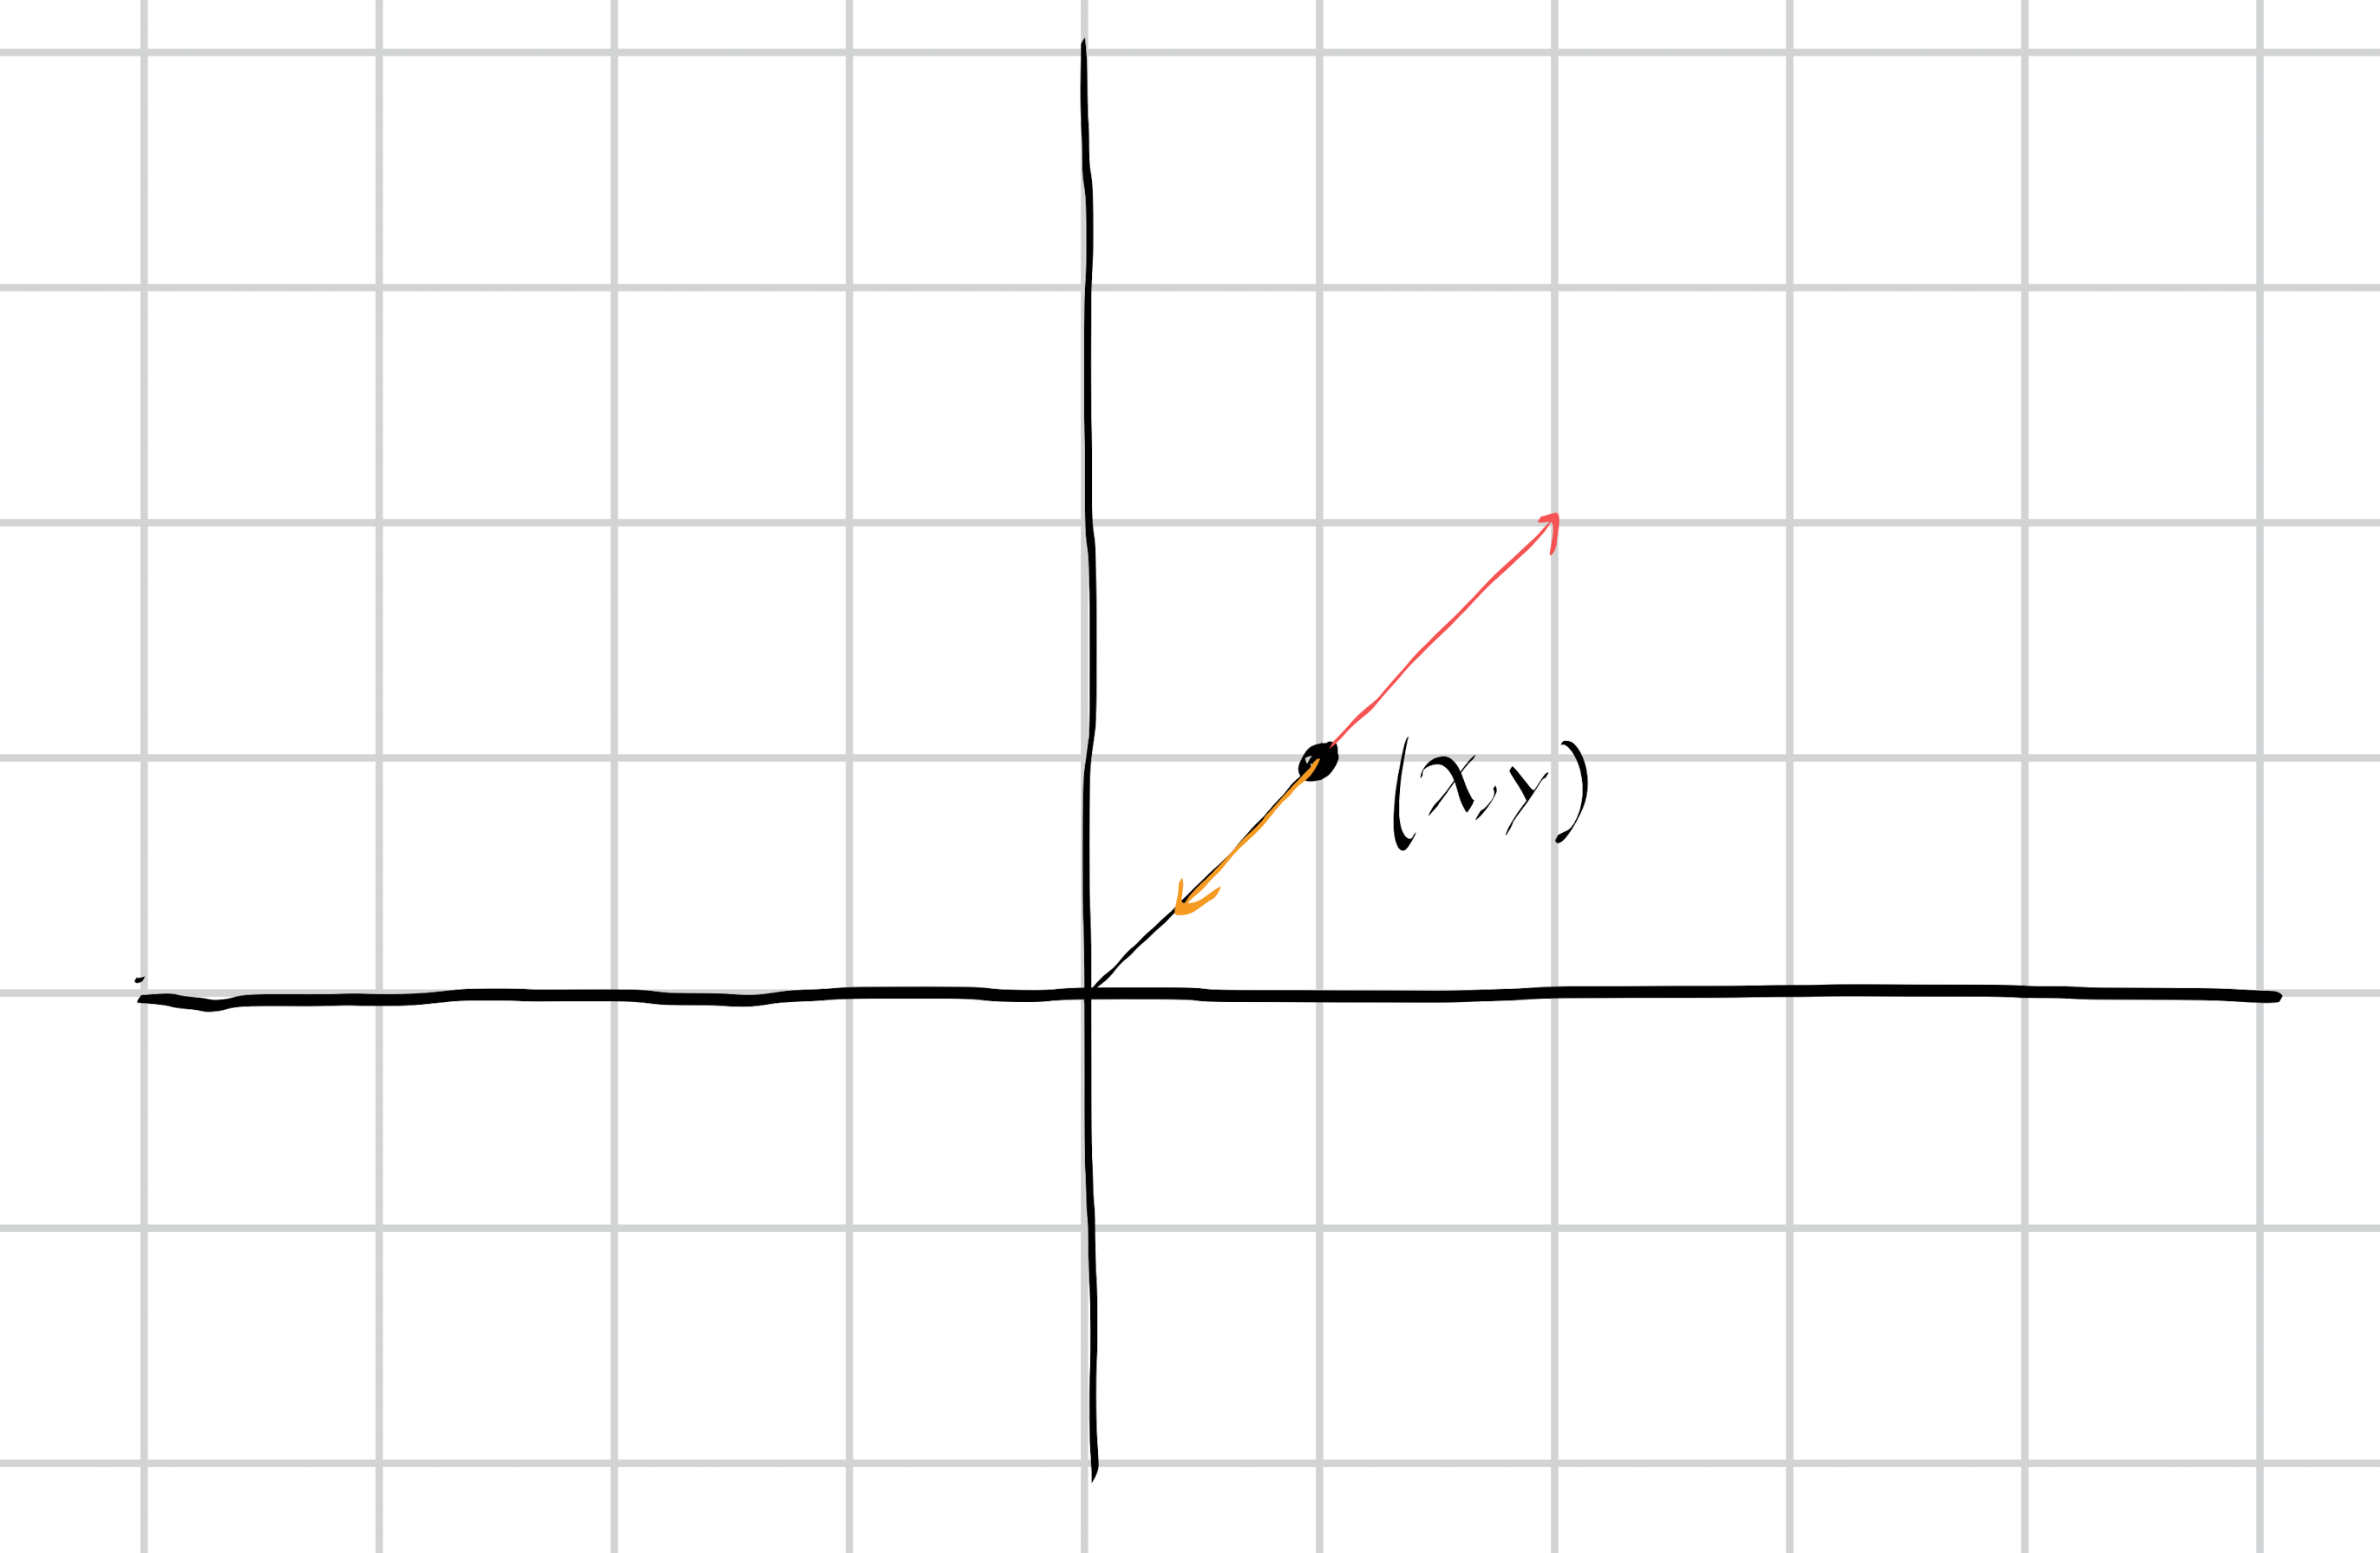
\includegraphics[width=7cm]{images/straight_line_solution.png}
\end{center}
Mathematically, we want to find a nonzero vector $\vec{v} = \begin{pmatrix}x\\y\end{pmatrix}$ and a number $\lambda$ such that
\begin{align*}
  A\vec{v} = \lambda \vec{v}.
\end{align*}
\begin{itemize}
  \item If $\lambda > 0$, then at $\vec{v}$, the vector field points away from the origin.
  \item If $\lambda < 0$, then at $\vec{v}$, the vector field points towards the origin.
\end{itemize}
The number $\lambda$ is the eigenvalue of $A$ and the vector $\vec{v}$ is the eigenvector corresponding to $\lambda$.
\begin{note}\hfill
  \begin{enumerate}[(1)]
    \item Given $A$, if $\vec{v}$ is an eigenvector for the eigenvalue $\lambda$, then so too is any $k\vec{v}$ for $k\in \R$.
    \item Given an eigenvector $\vec{v}$ for $\lambda$, the entire line through the origin $\Span\left(\vec{v}\right)$ are all eigenvectors for $\lambda$.
  \end{enumerate}
\end{note}
\begin{example}
  Consider the differential equation
  \begin{align*}
    \diff{\vec{Y}}{t} &= \begin{pmatrix}4 & -2 \\ 3 & -1\end{pmatrix} \vec{Y}.
  \end{align*}
  To find the eigenvalue of $A$, we take
  \begin{align*}
    \left(A - \lambda I\right)\vec{v} &= 0\\
    \begin{pmatrix}4-\lambda & -2 \\ 3 & -1 - \lambda\end{pmatrix} \begin{pmatrix}x\\y\end{pmatrix} &= 0,
  \end{align*}
  meaning we must have
  \begin{align*}
    \det\left(A - \lambda I\right) &= 0.
  \end{align*}
  to find non-trivial solutions. Calculating, we have
  \begin{align*}
    \det \begin{pmatrix}4-\lambda & -2 \\ 3 & -1-\lambda\end{pmatrix} &= \left(4-\lambda\right)\left(-1-\lambda\right) + 6\\
                                  &= \left(\lambda - 4\right)\left(\lambda + 1\right) + 6\\
                                  &= \lambda^2 - 3\lambda + 2\\
                                  &= \left(\lambda - 2\right)\left(\lambda - 1\right).
  \end{align*}
  We have eigenvalues of $\lambda_2 = 2$ and $\lambda_1 = 1$.\newline

  To find the corresponding eigenvectors, we start with $\lambda_1 = 1$.
  \begin{align*}
    \begin{pmatrix}3 & -2 \\ 3 & -2\end{pmatrix} \begin{pmatrix}x\\y\end{pmatrix} &= \begin{pmatrix}0\\0\end{pmatrix}\\
    3x - 2y &= 0\\
    3x -2y &= 0,
  \end{align*}
  meaning we have $y = \frac{3}{2}x$, or $\vec{v}_1 = \begin{pmatrix}2\\3\end{pmatrix}$. Similarly, we have
  \begin{align*}
    \begin{pmatrix}2 & -2 \\ 3 & -3\end{pmatrix} \begin{pmatrix}x\\y\end{pmatrix} &= \begin{pmatrix}0\\0\end{pmatrix},
  \end{align*}
  meaning we have $2x = 2y$, so $x = y$. Thus, $\vec{v}_{2} = \begin{pmatrix}1\\1\end{pmatrix}$.
\begin{definition}[Straight-Line Solution]
  If $\lambda$ is an eigenvalue associated with eigenvector $\vec{v} = \begin{pmatrix}x\\y\end{pmatrix}$. Then,
  \begin{align*}
    \vec{Y}_{\lambda}(t) &= e^{\lambda t}\vec{v}
  \end{align*}
  is a solution of $\diff{\vec{Y}}{t} = A\vec{Y}$.\newline

  If $A$ has two distinct eigenvalues, $\lambda_1$ and $\lambda_2$, then the corresponding eigenvectors are linearly independent, meaning there are two straight line solutions on the phase plane.
\end{definition}
\begin{exercise}
  Verify that the straight line solutions of the previous example are indeed straight line solutions.
\end{exercise}
Thus, we have $\vec{Y}_1(t) = e^{t} \begin{pmatrix}2\\3\end{pmatrix}$ and $\vec{Y}_2(t) = e^{2t} \begin{pmatrix}1\\1\end{pmatrix}$. Thus, the general solution is
\begin{align*}
  \vec{Y}(t) &= k_1\vec{Y}_1(t) + k_2\vec{Y}_2(t)\\
             &= \begin{pmatrix}2k_1e^{t} + k_2e^{2t}\\ 3k_1e^{t} + k_2e^{2t}\end{pmatrix}.
\end{align*}
Examining the phase plane, we see the following.
\begin{center}
  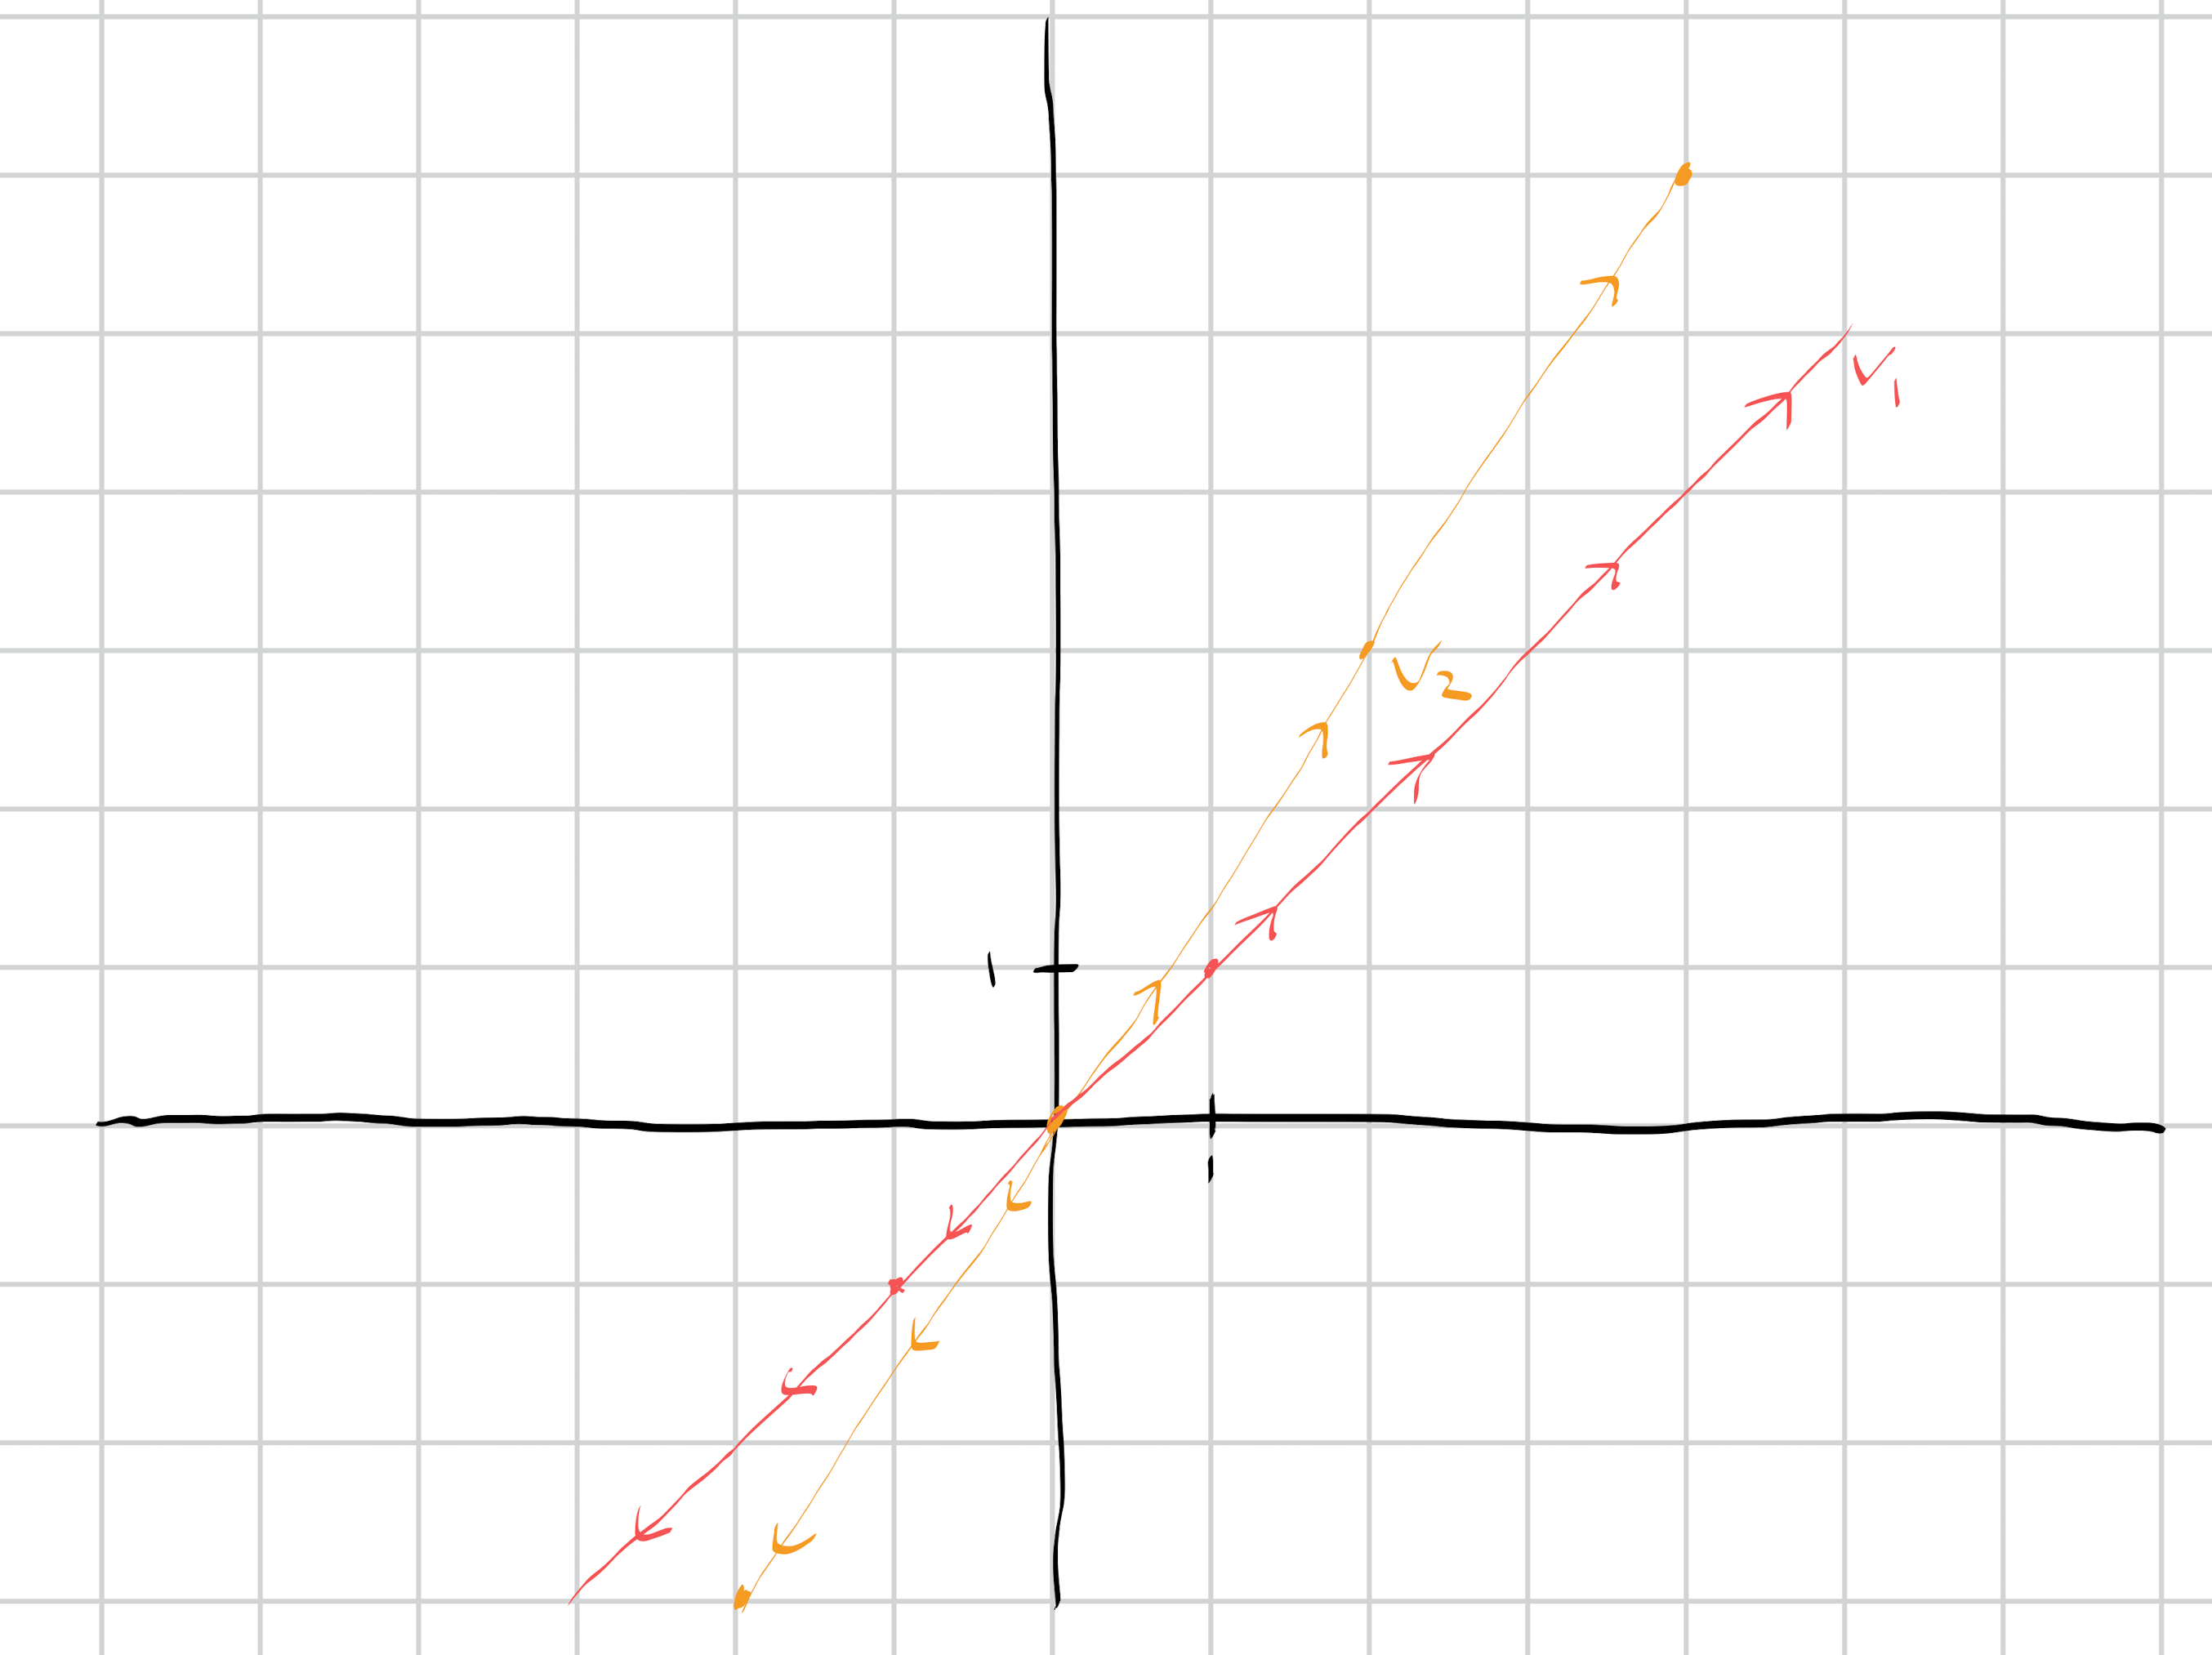
\includegraphics[width=7cm]{images/straight_line_2.png}
\end{center}
\end{example}
\begin{theorem}
  Suppose $A$ has a real eigenvalue $\lambda$ and associated vector $\vec{v}$.\newline

  Then, the linear system
  \begin{align*}
    \diff{\vec{Y}}{t} &= A\vec{Y}
  \end{align*}
  has the straight line solution
  \begin{align*}
    \vec{Y}(t) &= e^{\lambda t}\vec{v}.
  \end{align*}
  Moreover, if $\lambda_1$ and $\lambda_2$ are distinct real eigenvalues of $A$ with corresponding eigenvectors $\vec{v}_1$ and $\vec{v}_2$, the straight line solutions
  \begin{align*}
    \vec{Y}_1(t) &= e^{\lambda_1 t}\vec{v}_1\\
    \vec{Y}_2(t) &= e^{\lambda_2 t}\vec{v}_2,
  \end{align*}
  are linearly independent, so the general solution to the system is
  \begin{align*}
    \vec{Y}(t) &= k_1e^{\lambda_1 t}\vec{v}_1 + k_2e^{\lambda_2 t}\vec{v}_2.
  \end{align*}
\end{theorem}
\subsection{Phase Portraits for Linear Systems with Real Eigenvalues}%
Consider
\begin{align*}
  \diff{\vec{Y}}{t} &= A\vec{Y},\\
  A &= \begin{pmatrix}a & b \\ c & d\end{pmatrix}.
\end{align*}
Thus, we have the general eigenvalues
\begin{align*}
  \det \begin{pmatrix}a-\lambda & b \\ c & d-\lambda\end{pmatrix} &= 0\\
  \lambda^2 - \left(a+d\right)\lambda + \left(ad-bc\right) &= 0\\
  \left(\lambda - \frac{a + d}{2}\right)^2 &= \frac{4bc + \left(a-d\right)^2}{4}\\
  \lambda &= \frac{a+d}{2} \pm \frac{\sqrt{4bc + \left(a-d\right)^2}}{2}.
\end{align*}
\begin{itemize}
  \item We have complex eigenvalues if
\begin{align*}
  4bc + \left(a-d\right)^2 &< 0.
\end{align*}
\item  We have real eigenvalues if
\begin{align*}
  4bc + \left(a-d\right)^2 & > 0.
\end{align*}
\item We have repeated eigenvalues if
  \begin{align*}
    4bc + \left(a-d\right)^2 = 0
  \end{align*}
\end{itemize}
Note that for real eigenvalues with the same sign, the result
\begin{align*}
  \vec{Y}(t) &= k_1e^{\lambda_1 t}\vec{v}_1 + k_2e^{\lambda_2 t}\vec{v}_2
\end{align*}
provides that all solution curves are parallel to the ``faster'' growing/shrinking eigenvector, and are tangent to the ``slower'' growing/shrinking eigenvector.\newline

If we have a saddle (that is, one positive and one negative eigenvalue), then all solution curves are tangent to both eigenvectors, going in the direction of the positive/negative eigenvalue depending on its respective eigenvector.
\subsection{Phase Portraits for Systems with Complex Eigenvalues}%
We begin turning our attention to the case when
\begin{align*}
  4bc + \left(a-d\right)^2 &< 0.
\end{align*}
\begin{example}
  Consider the system
  \begin{align*}
    \diff{\vec{Y}}{t} &= \begin{pmatrix}2 & 2 \\ -4 & 6\end{pmatrix} \vec{Y}.
  \end{align*}
  Finding the eigenvalues, we take
  \begin{align*}
    \det\left(A - \lambda I\right) &= 0\\
    \left(2-\lambda\right)\left(6-\lambda\right) + 8 &= 0\\
    \lambda^2 - 8 \lambda + 20 &= 0\\
    \left(\lambda - 4\right)^2 &= -4\\
    \lambda &= 4 \pm 2i.
  \end{align*}
  Solving for the eigenvectors, we have
  \begin{align*}
    \begin{pmatrix}2 & 2 \\ -4 & 6\end{pmatrix} \begin{pmatrix}x\\y\end{pmatrix} &= \left(4+2i\right) \begin{pmatrix}x\\y\end{pmatrix}\\
    \left(-2-2i\right) x + 2y &= 0\\
    -4x + \left(2-2i\right)y &= 0\\
    y &= \left(1+i\right)x\\
    \vec{v}_1 &= \begin{pmatrix}1\\1+i\end{pmatrix}\\
    \begin{pmatrix}2 & 2 \\ -4 & 6\end{pmatrix} \begin{pmatrix}x\\y\end{pmatrix} &= \left(4-2i\right) \begin{pmatrix}x\\y\end{pmatrix}\\
    \left(-2 + 2i\right) + 2y &= 0\\
    -4x + \left(2+2i\right)y &= 0\\
    y &= \left(1 - i\right)x\\
    \vec{v}_2 &= \begin{pmatrix}1\\1 - i\end{pmatrix}.
  \end{align*}
  Using our system for straight-line solutions, we take
  \begin{align*}
    \vec{Y}_1(t) &= e^{\left(4+2i\right)t} \begin{pmatrix}1\\1+i\end{pmatrix}.
  \end{align*}
  We are dealing with an issue here --- namely, our equation exists in the real numbers, but we have a complex solution. To ameliorate this, we use the identity $e^{a+bi} = e^{a}\left(\cos b + i\sin b\right)$, to separate the equation to find
  \begin{align*}
    \vec{Y}_1\left(t\right) &= e^{4t}\left(\cos\left(2t\right) + i\sin\left(2t\right)\right) \begin{pmatrix}1\\1+i\end{pmatrix}\\
                            &= e^{4t}\cos\left(2t\right) \begin{pmatrix} 1\\1+i\end{pmatrix} + ie^{4t}\sin\left(2t\right) \begin{pmatrix}1\\1+i\end{pmatrix}\\
                            &= e^{4t}\cos\left(2t\right) \begin{pmatrix}1\\1\end{pmatrix} + ie^{4t}\cos\left(2t\right) \begin{pmatrix}0\\1\end{pmatrix} + ie^{4t}\sin\left(2t\right) \begin{pmatrix}1\\1\end{pmatrix} - e^{4t}\sin\left(2t\right) \begin{pmatrix}0\\1\end{pmatrix}\\
                            &= \underbrace{e^{4t} \begin{pmatrix}\cos\left(2t\right) \\ \cos\left(2t\right) - \sin\left(2t\right)\end{pmatrix}}_{\re\left(\vec{Y}_{1}(t)\right)} + i\underbrace{\left(e^{4t} \begin{pmatrix}\sin\left(2t\right)\\ \cos\left(2t\right) + \sin\left(2t\right)\end{pmatrix}\right)}_{\im\left(\vec{Y}_1(t)\right)}
  \end{align*}
  Note that $\re\left(\vec{Y}_1(0)\right)$ and $\im\left(\vec{Y}_1(0)\right)$ are linearly independent, and $\re\left(\vec{Y}_1(t)\right)$ and $\im\left(\vec{Y}_1(t)\right)$ are real solutions.\newline

  The general solution is, thus
  \begin{align*}
    \vec{Y}(t) &= k_1\re\left(\vec{Y}_1(t)\right) + k_2\im\left(\vec{Y}_1(t)\right).
  \end{align*}
\end{example}
\begin{theorem}[Complex Eigenvalues and Solutions]
  Suppose $\vec{Y}(t)$ is a complex-valued solution to the linear system of differential equation
  \begin{align*}
    \diff{\vec{Y}}{t} &= A\vec{Y}.
  \end{align*}
  Suppose
  \begin{align*}
    \vec{Y}(t) &= \re\left(\vec{Y}(t)\right) + i\im\left(\vec{Y}(t)\right),
  \end{align*}
  where both real and imaginary parts are real-valued functions of $t$. Then, $\re\left(\vec{Y}(t)\right)$ and $\im\left(\vec{Y}(t)\right)$ are both solutions to $\diff{\vec{Y}}{t} = A\vec{Y}$. The general solution is of the form
  \begin{align*}
    \vec{Y}(t) &= k_1\re\left(\vec{Y}(t)\right) + k_2\im\left(\vec{Y}(t)\right).
  \end{align*}
\end{theorem}
\begin{example}
  Let $\lambda = \alpha \pm i\beta$. The complex-valued solution is
  \begin{align*}
    \vec{Y}(t) &= e^{\left(\alpha + i\beta\right)t} \vec{v},
  \end{align*}
  where $\vec{v}$ is the eigenvector corresponding to $\lambda = \alpha + i\beta$.\newline

  Splitting up, we get
  \begin{align*}
    \vec{Y}(t) &= e^{\alpha t}e^{i\beta t}v\\
               &= e^{\alpha t}\left(\cos\left(\beta t\right) + i\sin\left(\beta t\right)\right)\vec{v}.
  \end{align*}
  Since $\vec{v}$ is constant, the long-term behavior of the solution curves is affected by $t$.
\begin{itemize}
  \item If $\alpha > 0$, then $e^{\alpha t} \rightarrow \infty$ as $t\rightarrow\infty$, so our solutions move away from the origin. If $\beta \neq 0$, then they do so in a spiral pattern.
    \begin{center}
      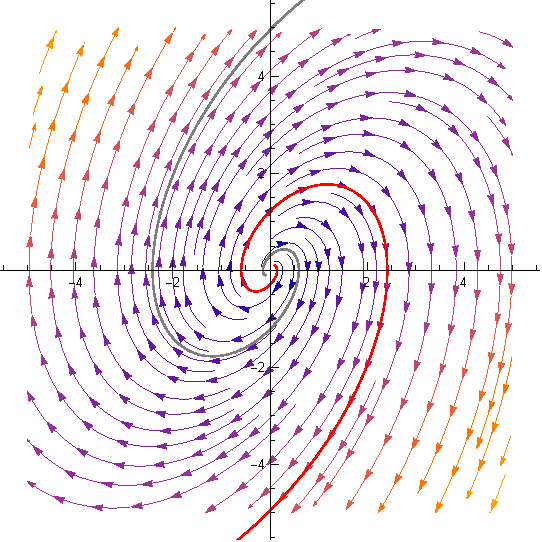
\includegraphics[width=10cm]{images/positive_real_part.pdf}
    \end{center}
  \item If $\alpha < 0$, then $e^{\alpha t}\rightarrow 0$ as $t\rightarrow\infty$, so our solutions move toward the origin. If $\beta \neq 0$, they do so in a spiral pattern.
    \begin{center}
      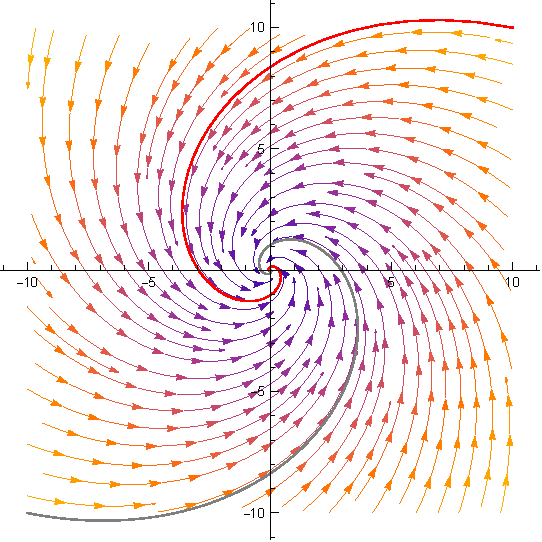
\includegraphics[width=10cm]{images/negative_real_part.pdf}
    \end{center}
  \item If $\alpha = 0$ and $\beta \neq 0$, we have a purely periodic solution.
    \begin{center}
      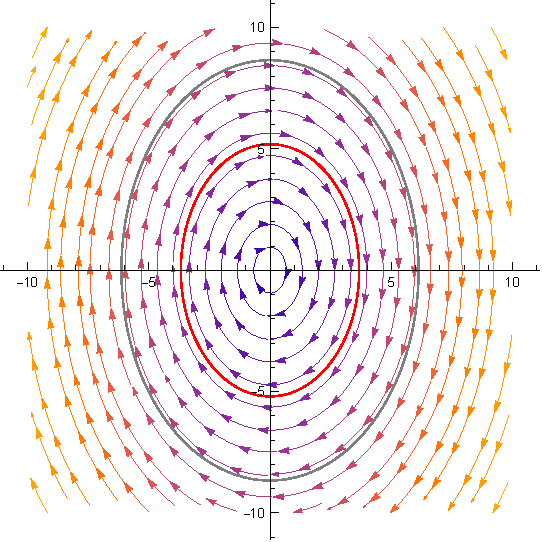
\includegraphics[width=10cm]{images/zero_real_part.pdf}
    \end{center}
\end{itemize}
\end{example}
Recall that when we find the eigenvalues of a matrix $A$, we see that
\begin{align*}
  \det \begin{pmatrix}a-\lambda & b \\ c & d-\lambda\end{pmatrix} &= 0\\
  \lambda^2 - \underbrace{\left(a+d\right)}_{\tr(A)}\lambda + \underbrace{\left(ad-bc\right)}_{\det (A)} &= 0.
\end{align*}
Solving using the quadratic formula we get
\begin{align*}
  \lambda &= \frac{\left(a+d\right) \pm \sqrt{\left(a+d\right)^2 - 4\left(ad-bc\right)}}{2}.
\end{align*}
We can see that the real part of $\lambda$ is
\begin{align*}
  \re\left(\lambda\right) &= \frac{a+d}{2}.
\end{align*}
This is a quick way to evaluate a whether the origin is a spiral source vs. spiral sink.
\subsection{Phase Portraits for Repeated Eigenvalues}%
Consider
\begin{align*}
  \diff{\vec{Y}}{t} &= \begin{pmatrix}-2 & 1 \\ 0 & -2\end{pmatrix} \vec{Y}
\end{align*}
our linear system. There are repeated eigenvalues of $\lambda = -2$. The corresponding eigenvector is
\begin{align*}
  \vec{v} &= \begin{pmatrix}1\\0\end{pmatrix}.
\end{align*}
We can see the straight line solution of the form
\begin{align*}
  \vec{Y}_1(t) &= e^{-2t} \begin{pmatrix}1\\0\end{pmatrix}.
\end{align*}
To see the general solutions, we start by converting into the system.
\begin{align*}
  \diff{x}{t} &= -2x + y\\
  \diff{y}{t} &= -2y.
\end{align*}
Since this system is partially decoupled, we are indeed able to solve it.
\begin{align*}
  y(t) &= k_1e^{-2t}\\
  \diff{x}{t} &= -2x + k_1e^{-2t}\\
  \diff{x}{t} + 2x &= k_1e^{-2t}\\
  e^{2t}\diff{x}{t} + 2xe^{2t} &= k_1\\
  \diff{}{t}\left(xe^{2t}\right) &= k_1\\
  xe^{2t} &= k_1t + k_2\\
  x &= k_1te^{-2t} + k_2e^{-2t}.
\end{align*}
Our general solution is, thus
\begin{align*}
  \vec{Y}(t) &= \begin{pmatrix}k_1te^{-2t} + k_2e^{-2t}\\ k_2e^{-2t}\end{pmatrix}.
\end{align*}
Including the initial condition of $x(0) = x_0$, $y(0) = y_0$, we get
\begin{align*}
  \vec{Y}(t) &= \begin{pmatrix}y_0te^{-2t} + x_0e^{-2t} \\ y_0e^{-2t}\end{pmatrix}\\
             &= te^{-2t} \underbrace{\begin{pmatrix}y_0\\0\end{pmatrix}}_{\vec{v}} + e^{-2t} \underbrace{\begin{pmatrix}x_0\\y_0\end{pmatrix}}_{\vec{Y}(0)}.
\end{align*}
\begin{theorem}
  Let $\diff{\vec{Y}}{t} = A\vec{Y}$ be a linear system where $A$ is a $2\times 2$ matrix with a repeated real eigenvalue $\lambda$, but with only one eigenline. Then, the general solution is the following.
  \begin{align*}
    \vec{Y}(t) &= e^{\lambda t} \vec{v}_0 + te^{\lambda t}\vec{v}_1,
  \end{align*}
  where $\vec{v}_0$ is an arbitrary initial condition, and $\vec{v}_1$ is determined as follows:
  \begin{align*}
    \vec{v}_1 &= \left(A- \lambda I\right)\vec{v}_0.
  \end{align*}
  If $\vec{v}_1 = 0$, then $\vec{v}_0$ is an eigenvector, and $\vec{Y}(t)$ is a straight line solution. Otherwise, $\vec{v}_1$ is an eigenvector.
\end{theorem}
\begin{example}
  Let
  \begin{align*}
    \diff{\vec{Y}}{t} &= \begin{pmatrix}-1 & 2 \\ -2 & 3\end{pmatrix} \vec{Y}.
  \end{align*}
  The eigenvalues of this matrix are $\lambda = 1$. We let
  \begin{align*}
    \vec{v}_0 &= \begin{pmatrix}x_0\\y_0\end{pmatrix},
  \end{align*}
  and
  \begin{align*}
    \vec{v}_1 &= \left(A - \lambda I\right)\vec{v}_0\\
              &= \begin{pmatrix}-2 & 2 \\ -2 & 2\end{pmatrix} \begin{pmatrix}x_0\\y_0\end{pmatrix}\\
              &= \begin{pmatrix}-2x_0 + 2y_0 \\ -2x_0 + 2y_0\end{pmatrix}.
  \end{align*}
  Thus, our solution is
  \begin{align*}
    \vec{Y}(t) &= e^{t} \begin{pmatrix}x_0\\y_0\end{pmatrix} + te^{t} \begin{pmatrix}-2x_0 + 2y_0\\-2x_0 + 2y_0\end{pmatrix}.
  \end{align*}
  To create solutions, we let the initial condition change over time, and find the desired eigenvectors.\newline

  For instance, if our initial condition is $\vec{v}_0 = \begin{pmatrix}1\\0\end{pmatrix}$, then $\vec{v}_1 = \begin{pmatrix}-2\\-2\end{pmatrix}$, and our solutions look as follows.
  \begin{center}
    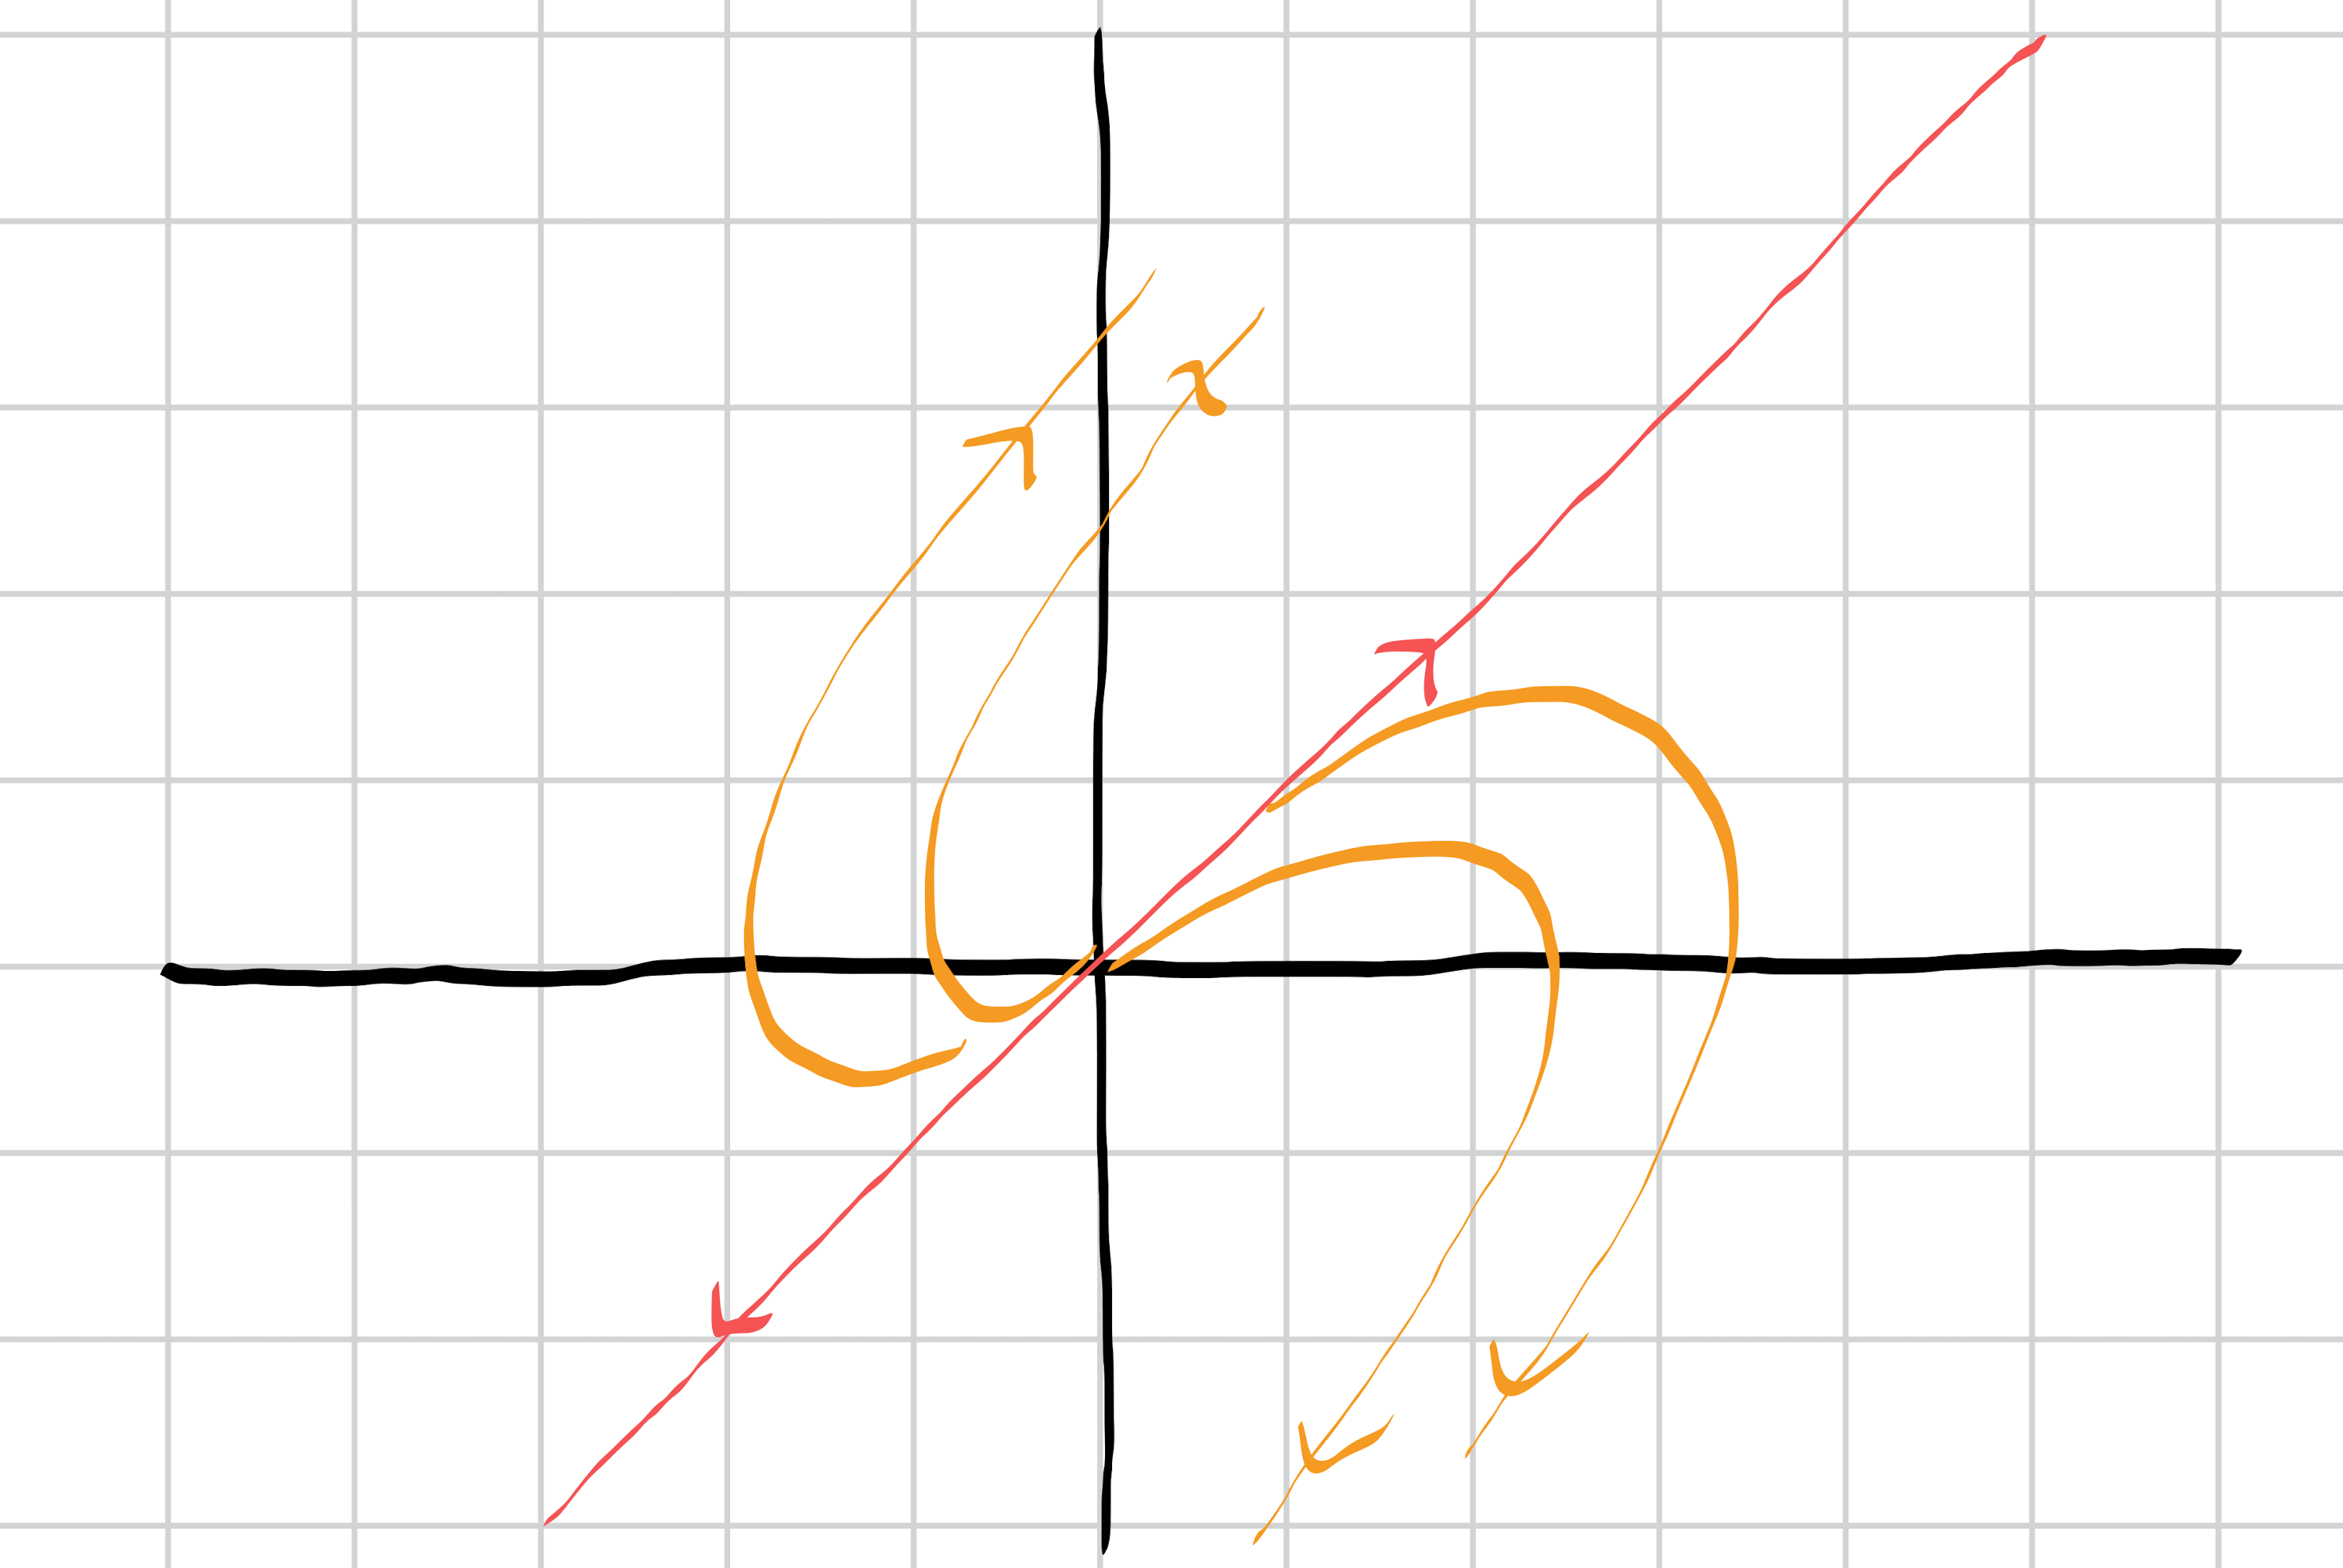
\includegraphics[width=10cm]{images/nodal_source.png}
  \end{center}
  In this scenario, we say the origin is a nodal source.
\end{example}
\begin{example}[Qualitative Analysis]
  Note that we can take
  \begin{align*}
    \vec{Y}(t) &= e^{\lambda t}\vec{v}_0 + te^{\lambda t}\vec{v}_1\\
               &= e^{\lambda t}\left(\vec{v}_1 + t\vec{v}_1\right).
  \end{align*}
  As $t\rightarrow\infty$, the solution asymptotically approaches the direction $\vec{v}_1$. This is more readily apparent if $\lambda > 0$.\newline

  For $\lambda < 0$, we have nodal sinks. To find the initial direction for this case, we plug in the initial condition and evaluate the vector field at the particular point.
  \begin{center}
    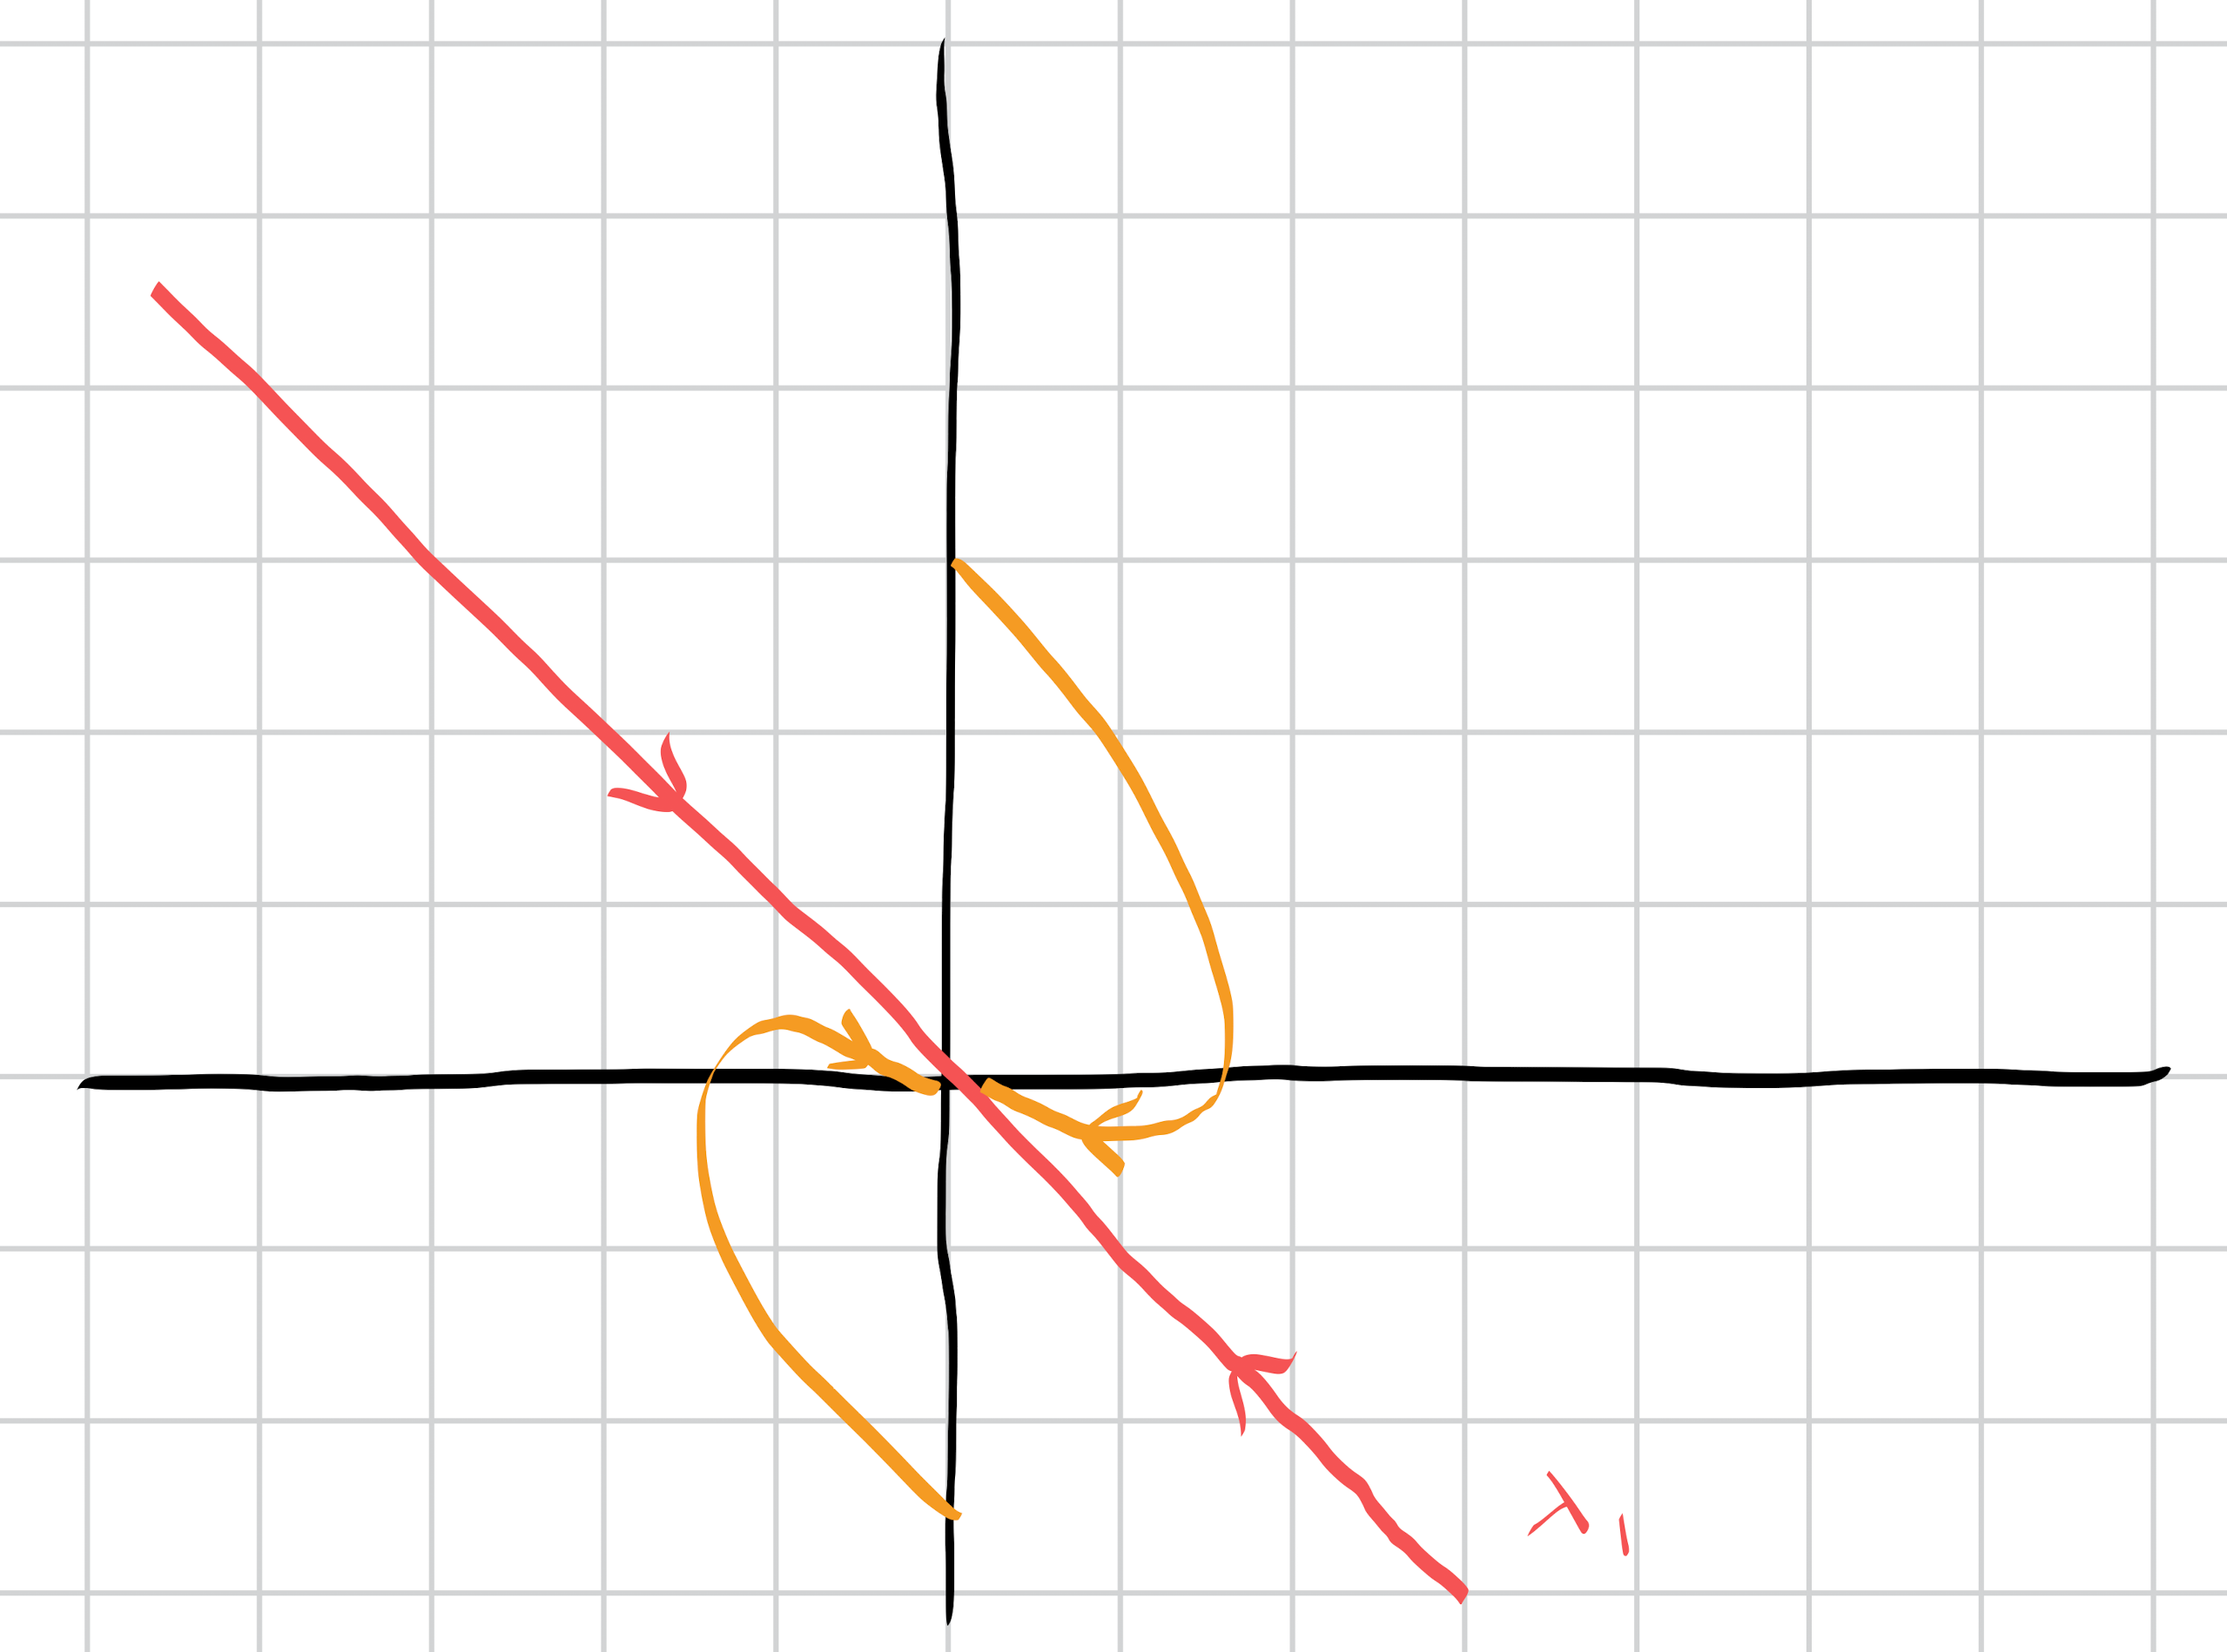
\includegraphics[width=7cm]{images/nodal_sink_1.png}\break
    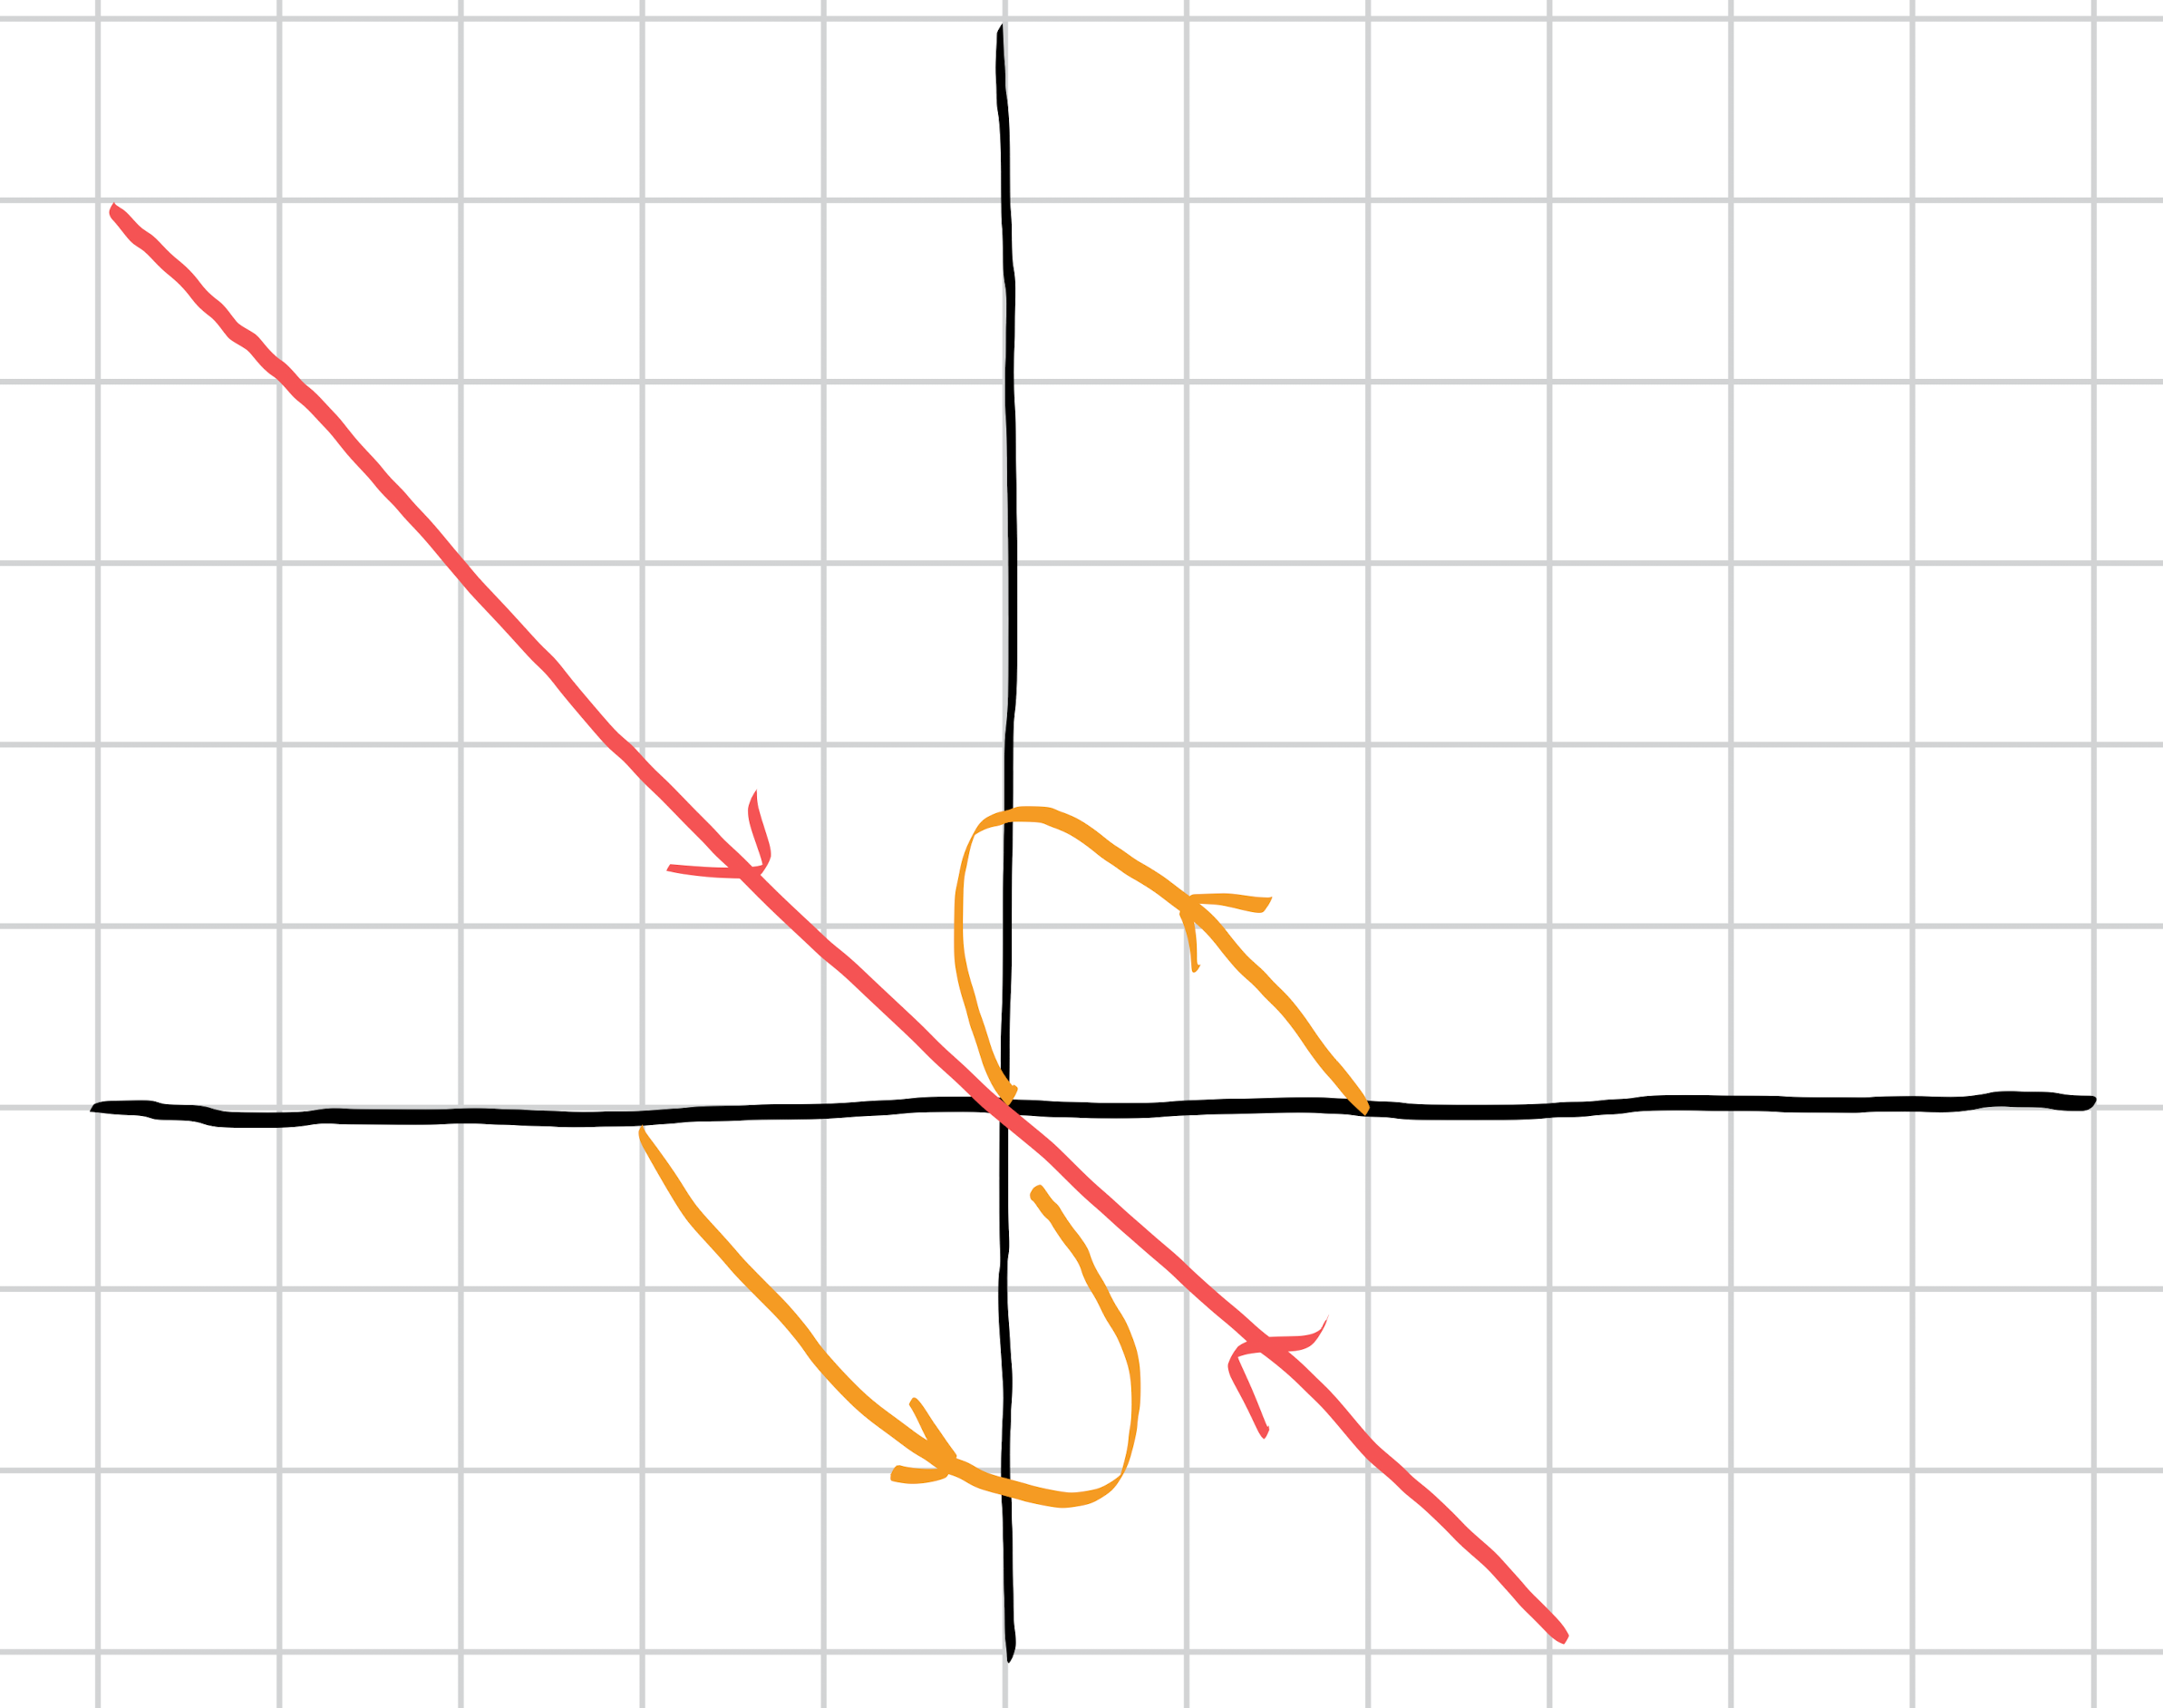
\includegraphics[width=7cm]{images/nodal_sink_2.png}
  \end{center}
\end{example}
\begin{example}[Scaled Identity]
  Consider the equation
  \begin{align*}
    \diff{\vec{Y}}{t} &= \underbrace{\begin{pmatrix}a & 0 \\ 0 & a\end{pmatrix}}_{A} \vec{Y}.
  \end{align*}
  The eigenvalues of $A$ are repeated with value $a$. Note that since this is a scaled identity matrix, the eigenvectors are every vector in the plane.\newline

  Thus, we can select linearly independent eigenvectors. We let
  \begin{align*}
    \vec{v}_1 &= \begin{pmatrix}1\\0\end{pmatrix}\\
    \vec{v}_2 &= \begin{pmatrix}0\\1\end{pmatrix}.
  \end{align*}
  Note that $\vec{v}_1$ and $\vec{v}_2$ are linearly independent.\newline

  Since every vector is an eigenvector, every solution is a straight line solution. The general solution is
  \begin{align*}
    \vec{Y}(t) &= k_1e^{at} \begin{pmatrix}1\\0\end{pmatrix} + k_2e^{at} \begin{pmatrix}0\\1\end{pmatrix}\\
               &= \begin{pmatrix}k_1e^{at} \\ k_2e^{at}\end{pmatrix}.
  \end{align*}
  In this case, our phase portrait has its phase lines as follows. 
  \begin{center}
    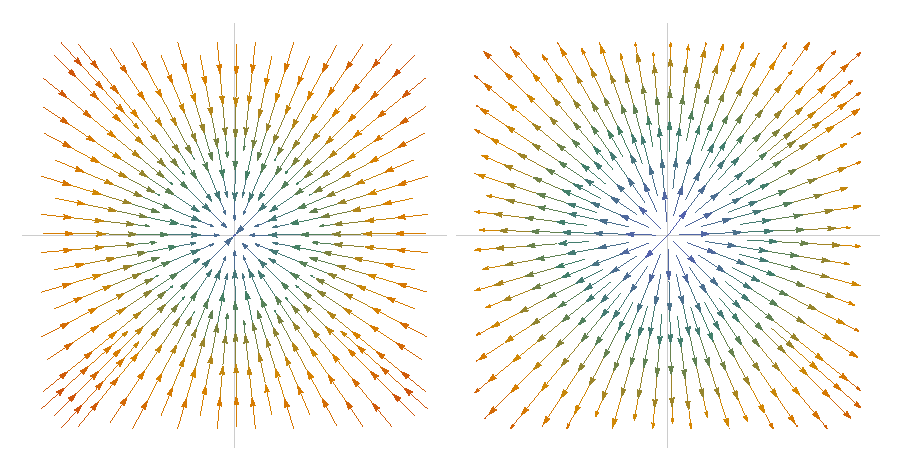
\includegraphics[height=7cm]{images/source_star_sink_star.pdf}
  \end{center}
  We say these are sink star and source star points respectively.
\end{example}
\begin{example}
  Consider the equation
  \begin{align*}
    \diff{\vec{Y}}{t} &= \begin{pmatrix}-3 & 1 \\ 3 & -1\end{pmatrix}\vec{Y},
  \end{align*}
  which has eigenvalues $\lambda_1 = 0$ and $\lambda_2 = 4$, with eigenvectors
  \begin{align*}
    \vec{v}_1 &= \begin{pmatrix}1\\3\end{pmatrix}\\
    \vec{v}_2 &= \begin{pmatrix}-1\\1\end{pmatrix}.
  \end{align*}
  The general solution is of the form
  \begin{align*}
    \vec{Y}(t) &= k_1 \begin{pmatrix}1\\3\end{pmatrix} + k_2 e^{-4t}\begin{pmatrix}-1\\1-1\\1\end{pmatrix}.
  \end{align*}
  We can see that if $k_2 = 0$, then we have equilibrium solutions. Thus, the eigenline for $\vec{v}_1$ consist of all the equilibrium solutions. The phase diagram looks as follows.
  \begin{center}
    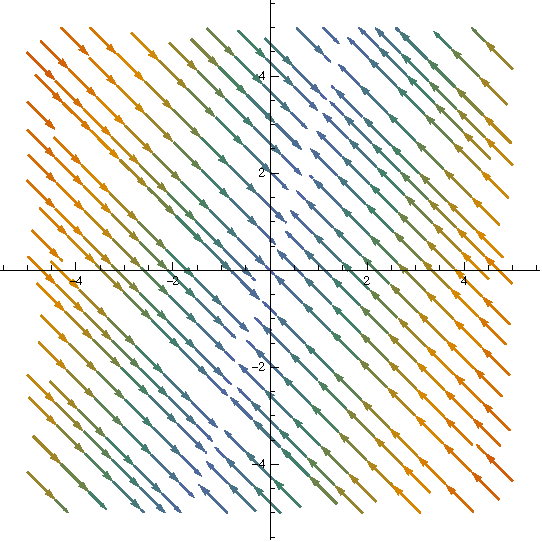
\includegraphics[width=10cm]{images/zero_eigenvalue.pdf}
  \end{center}
\end{example}
\begin{example}
  Consider the system
  \begin{align*}
    \diff{\vec{Y}}{t} &= \begin{pmatrix}0 & 2 \\ 0 & 0\end{pmatrix}\vec{Y},
  \end{align*}
  with repeated eigenvalues $\lambda = 0$. We only have one eigenvector
  \begin{align*}
    \vec{v}  &= \begin{pmatrix}1\\0\end{pmatrix}.
  \end{align*}
  Let $\vec{v}_0 = \begin{pmatrix}x_0\\y_0\end{pmatrix}$. Then, $v_1 = \begin{pmatrix}2y_0\\0\end{pmatrix}$. Thus, our general solution is
  \begin{align*}
    \vec{Y}(t) &= k_1 \begin{pmatrix}x_0\\y_0\end{pmatrix} + 2t \begin{pmatrix}y_0\\0\end{pmatrix}.
  \end{align*}
  The phase diagram looks as follows.
  \begin{center}
    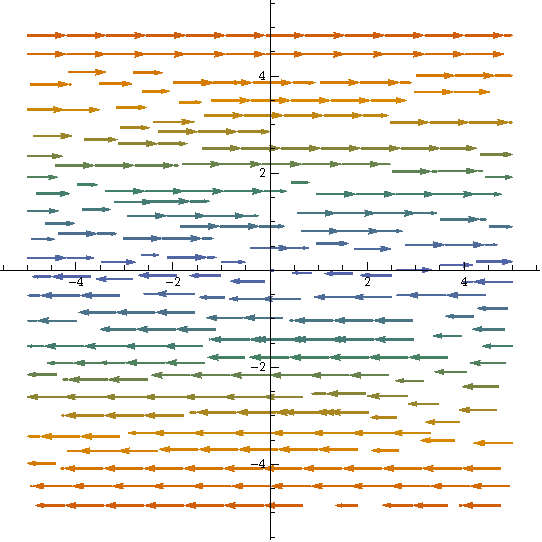
\includegraphics[width=10cm]{images/one_eigenvector_zero_eigenvalue.pdf}
  \end{center}
\end{example}
\begin{example}
  Consider the system
  \begin{align*}
    \diff{\vec{Y}}{t} &= \begin{pmatrix}0 & 0 \\ 0 & 0\end{pmatrix} \vec{Y}.
  \end{align*}
  Then, there is one repeated eigenvalue of $0$, and every point is an equilibrium solution.
\end{example}
\subsection{The Trace-Determinant Plane}%
Recall that in the expression
\begin{align*}
  \diff{\vec{Y}}{t} &= \begin{pmatrix}a & b \\ c & d\end{pmatrix} \vec{Y},
\end{align*}
the eigenvalues of $A$ are the solutions to
\begin{align*}
  \lambda^2 - \left(a + d\right)\lambda + \left(ad - bc\right) &= 0\\
  \lambda^2 - T\lambda + D &= 0\\
  \lambda &= \frac{T}{2} \pm \sqrt{\frac{T^2}{4} - D}.
\end{align*}
\begin{itemize}
  \item If we have complex eigenvalues with real part $\frac{T}{2}$,
    \begin{itemize}
      \item  for $T < 0$, we have a spiral sink;
      \item for $T > 0$, we have a spiral source;
      \item for $T = 0$, we have a center.
    \end{itemize}
  \item If we have repeated eigenvalues, then
    \begin{itemize}
      \item for $T < 0$, we have a nodal sink (or a sink star point, if every vector is an eigenvector);
      \item for $T > 0$, we have a nodal source (or a source star point, if every vector is an eigenvector);
      \item for $T = 0$, we have the special cases discussed earlier.
    \end{itemize}
  \item If we have two real eigenvalues,
    \begin{itemize}
      \item for $T > 0$ and $D > 0$, we have two positive eigenvalues,\footnote{Recall that the trace is the sum of the eigenvalues and the determinant is the product of the eigenvalues.} so we have a source;
      \item for $T > 0$ and $D = 0$, we have one zero eigenvalue and one positive eigenvalue, so we have a line of unstable equilibria;
      \item for $T > 0$ and $D < 0$, we have one positive eigenvalue and one negative eigenvalue, so we have a saddle;\newline

      \item for $T < 0$ and $D > 0$, we have two negative eigenvalues, so we have a sink;
      \item for $T < 0$ and $D = 0$, we have one zero eigenvalue and one negative eigenvalue, so we have a line of stable equilibria;
      \item for $T < 0$ and $D < 0$, we have one positive eigenvalue and one negative eigenvalue, so we have a saddle.
    \end{itemize}
\end{itemize}
The following diagram\footnote{Taken from \href{https://tex.stackexchange.com/questions/347201/drawing-the-trace-determinant-diagram-on-latex}{\LaTeX Stack Exchange}.} visualizes the trace-determinant plane.
\begin{center}
  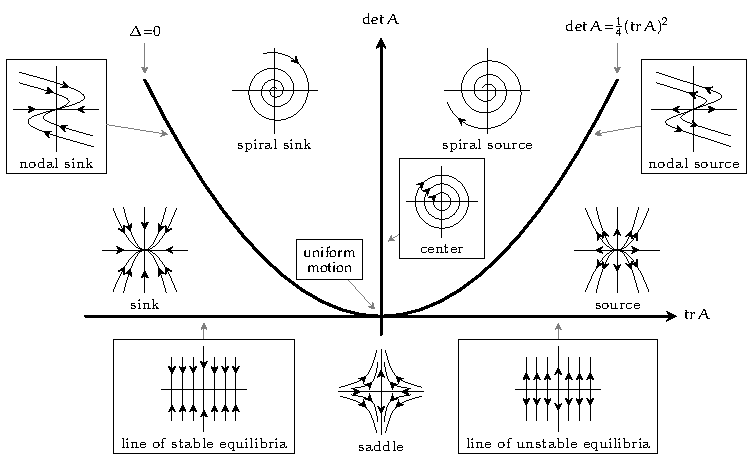
\includegraphics[width=15cm]{images/trace_determinant.pdf}
\end{center}
\begin{example}[Bifurcations for Systems of Equations]
  Consider the family of systems (where $a$ is a parameter)
  \begin{align*}
    \diff{\vec{Y}}{t} &= \begin{pmatrix}-2 & a \\ -2 & 0\end{pmatrix} \vec{Y}.
  \end{align*}
  We find that
  \begin{align*}
    \det A &= 2a\\
    \tr A &= -2.
  \end{align*}
  Using the trace-determinant plane, we find the equation
  \begin{align*}
    \det A &= \frac{1}{4}\left(\tr A\right)^2\\
    2a &= 1
  \end{align*}
  characterizes the bifurcation values. 
  \begin{itemize}
    \item If $a > \frac{1}{2}$, the origin is a spiral sink.
    \item If $0 < a < \frac{1}{2}$, the origin is a sink.
    \item If $a < 0$, the origin is a saddle.
    \item If $a = \frac{1}{2}$, the origin is a nodal sink or sink star point.
    \item If $a = 0$, we have a line of attracting fixed points (as one of our eigenvalues is negative).
  \end{itemize}
  The bifurcation values are thus at $a = 0$ and $a = \frac{1}{2}$.
  \begin{center}
    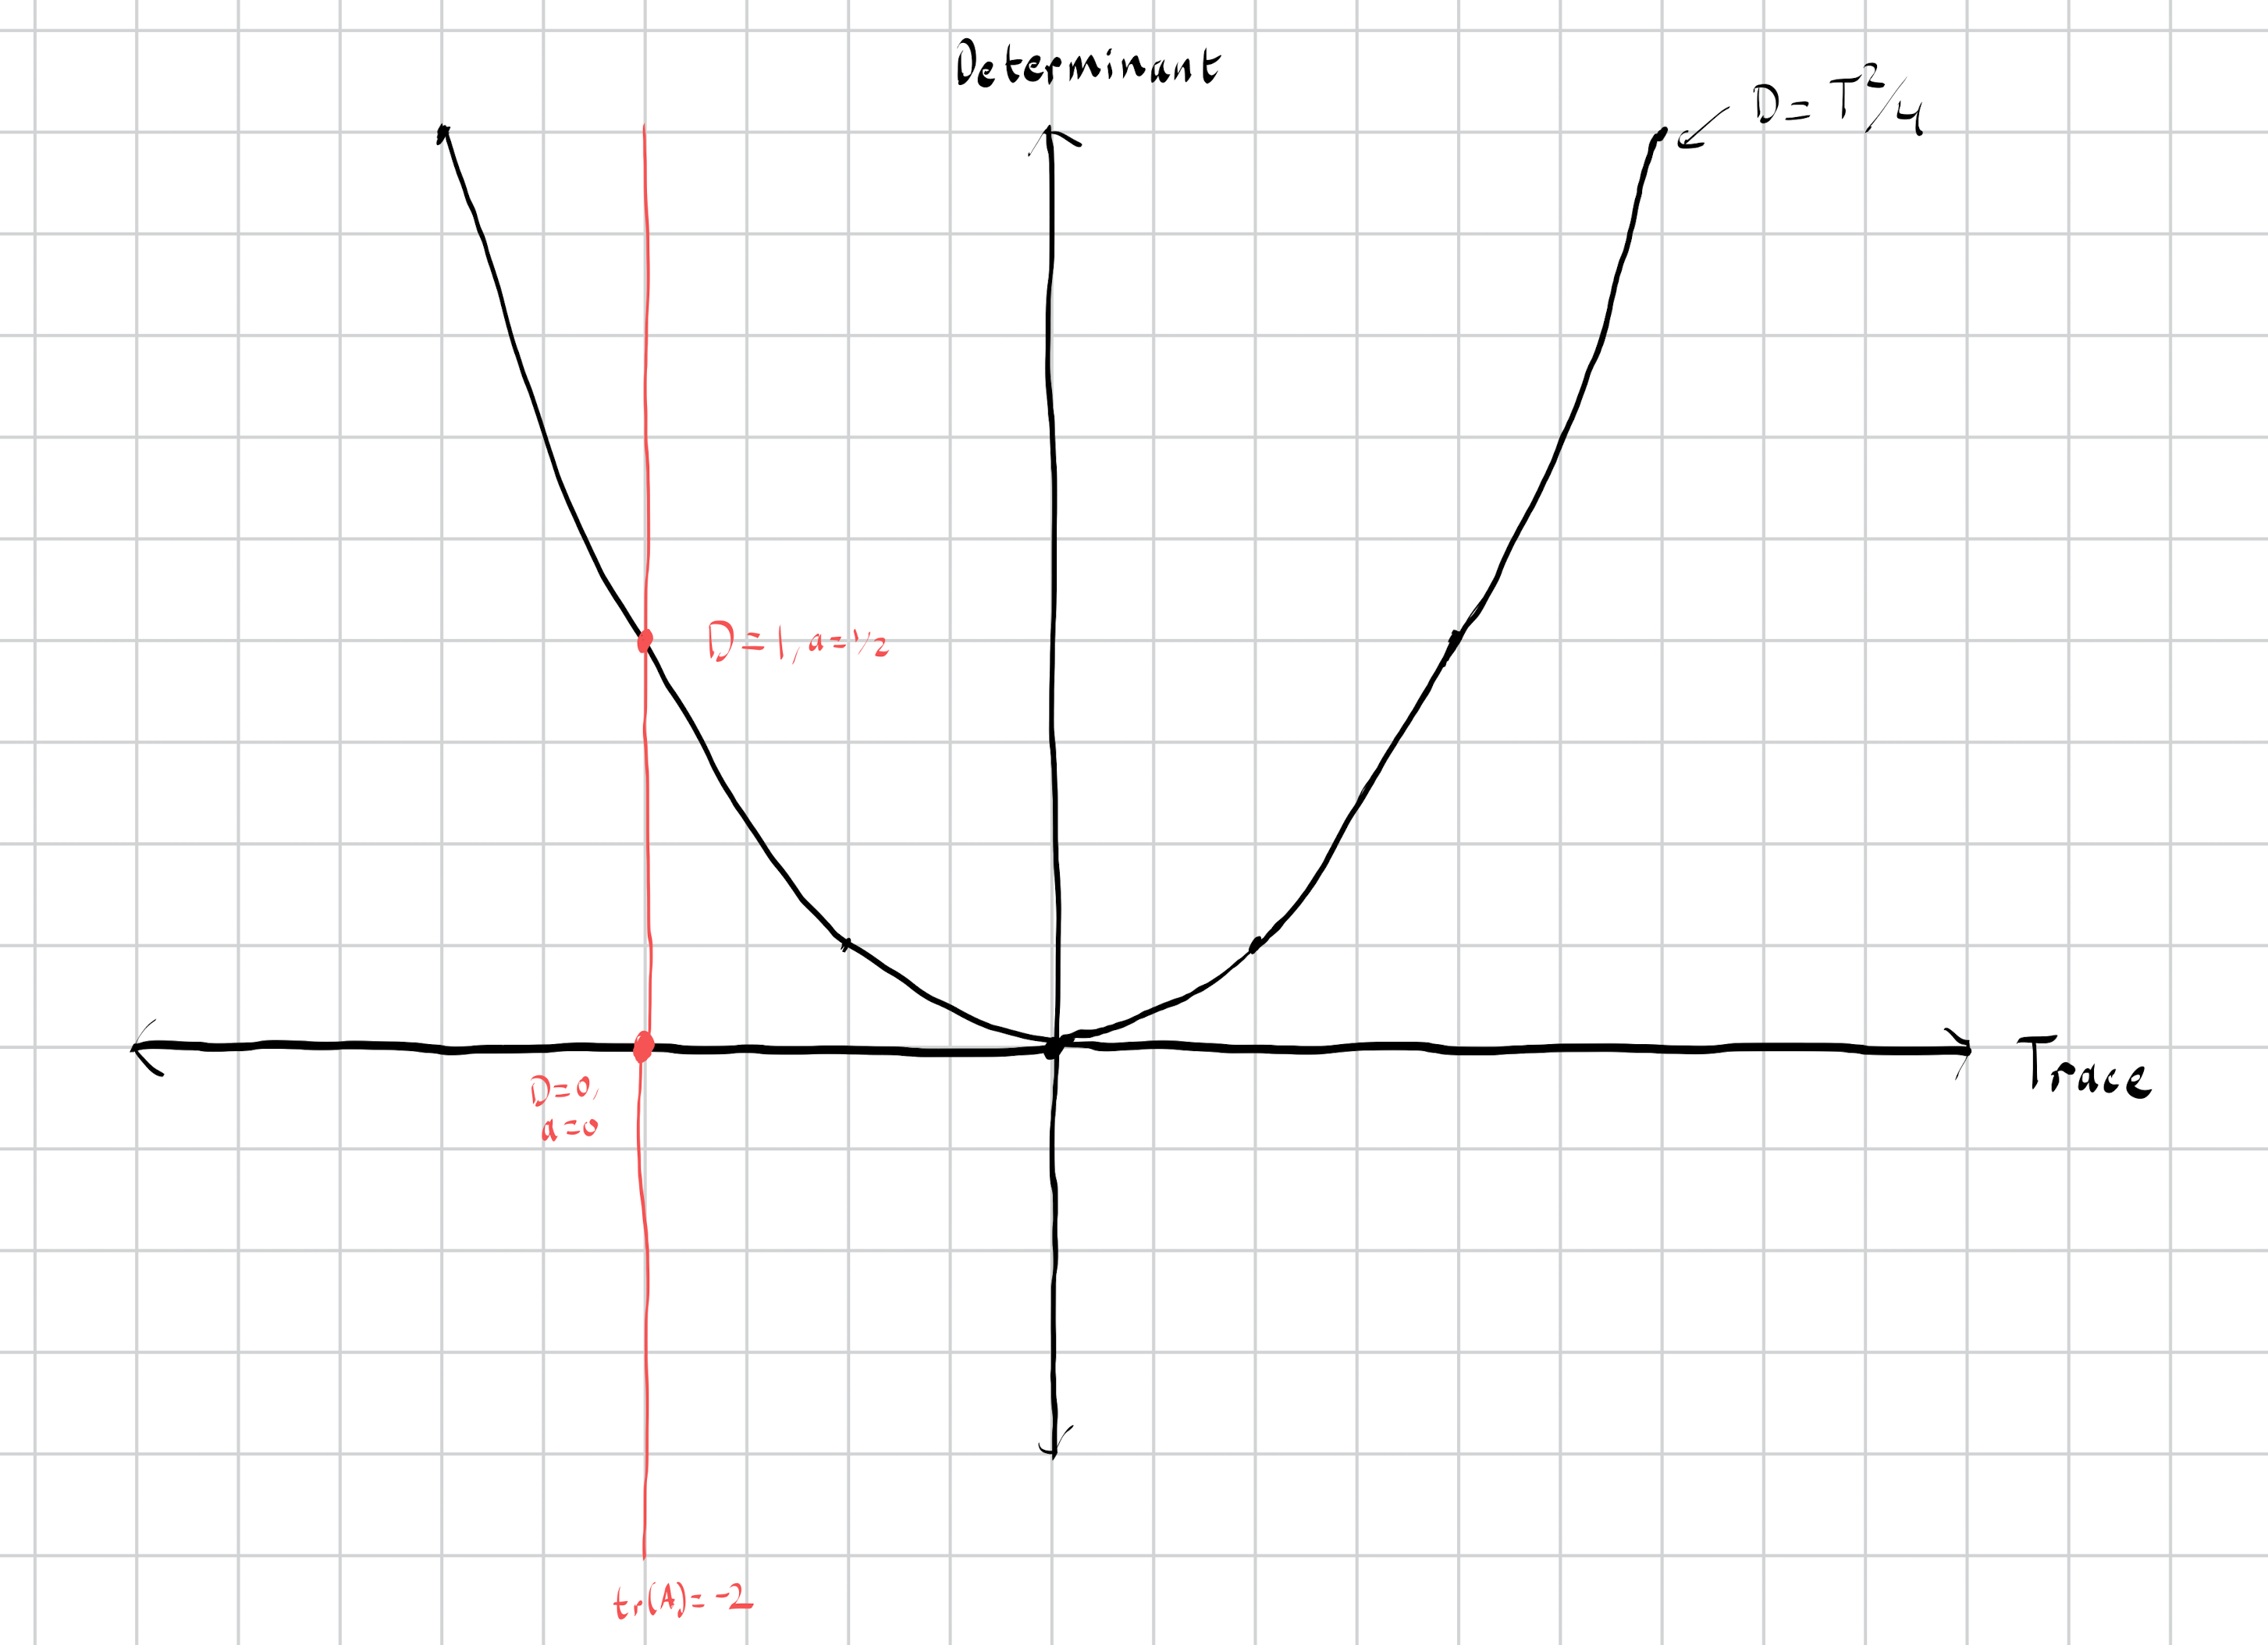
\includegraphics[width=10cm]{images/bifurcation_trace_determinant_1.png}
  \end{center}
\end{example}
\section{Understanding Nonlinear Systems}%
\subsection{Equilibrium Point Analysis}%
We will start by examining a special system known as the Van der Pol system of equations.
\begin{align*}
  \diff{x}{t} &= y\\
  \diff{y}{t} &= -x + \left(1-x^2\right)y.
\end{align*}
\begin{center}
  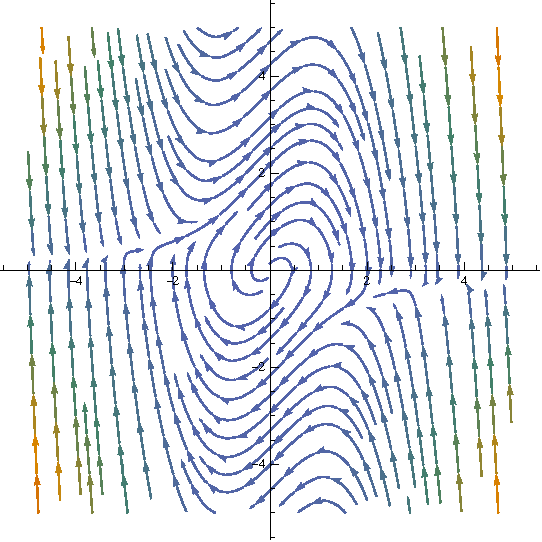
\includegraphics[width=10cm]{images/van_der_pol_equation.pdf}
\end{center}
We can start by finding the equilibrium solutions. Taking $\diff{x}{t} = 0$, we find $y = 0$, from which we place into $\diff{y}{t} = -x + \left(1-x^2\right)\left(0\right) = 0$, so $x = 0$.\newline

The only equilibrium point is the origin. Note that we can see the origin is a type of spiral source as we zoom in close to the origin.
\begin{center}
  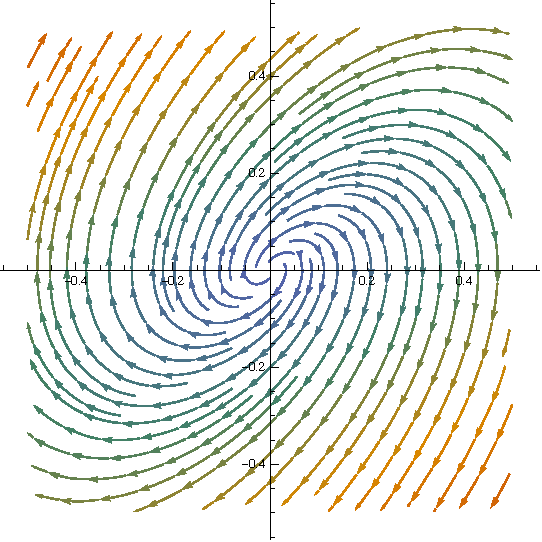
\includegraphics[width=10cm]{images/van_der_pol_equation_near_origin.pdf}
\end{center}
We can justify this by approximating the nonlinear system with a linear system.\newline

When we are very close to the origin such as at $x=y=0.1$, the term $x^2 y$ is orders of magnitude smaller than $x$ and $y$. We can then analyze the linearized system
\begin{align*}
  \diff{x}{t} &= y\\
  \diff{y}{t} &= -x + y,
\end{align*}
which is
\begin{align*}
  \diff{\vec{Y}}{t} &= \begin{pmatrix}0 & 1 \\ -1 & 1\end{pmatrix} \vec{Y}.
\end{align*}
Solving this system of equations, we find eigenvalues 
\begin{align*}
  \det\left(A - \lambda I\right) &= \lambda\left(\lambda - 1\right) + 1\\
  \lambda^2 - \lambda + 1 &= 0\\
  \left(\lambda - \frac{1}{2}\right)^2 &= -\frac{3}{4}\\
  \lambda &= \frac{1}{2} \pm \frac{\sqrt{3}}{2}i.
\end{align*}
We can see that this is a complex solution, and specifically that the origin is a spiral source (as the real part is positive). Note that, near the origin, we can see that the linearization (on the right) and the original system (on the left) are very similar.
\begin{center}
  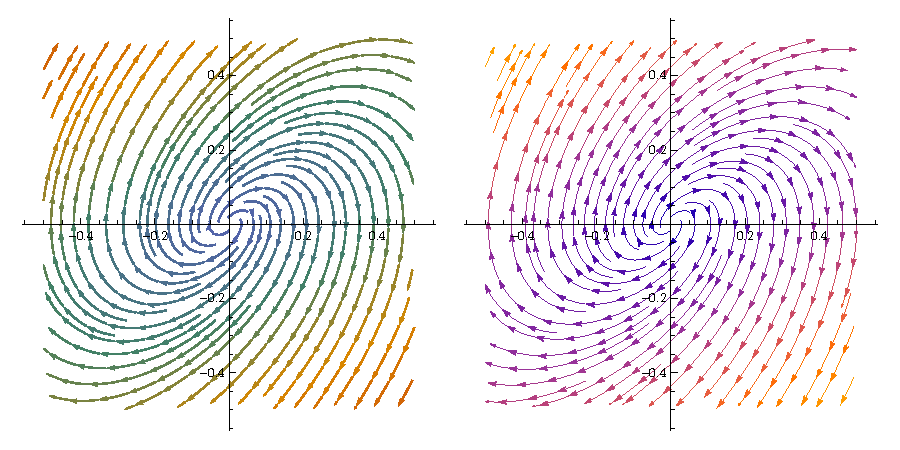
\includegraphics[width=15cm]{images/van_der_pol_linearization.pdf}
\end{center}
Considering an arbitrary nonlinear system
\begin{align*}
  \diff{x}{t} &= f\left(x,y\right)\\
  \diff{y}{t} &= g\left(x,y\right)
\end{align*}
with equilibrium point $\left(a,b\right)$, where $f\left(a,b\right) = 0 = g\left(a,b\right)$, we can use techniques from multivariable calculus to find the linear approximation of $f\left(x,y\right)$ near $\left(a,b\right)$.
\begin{align*}
  f\left(x,y\right) &\approx f\left(a,b\right) + \pd{f}{x}\Bigr\vert_{\left(a,b\right)}\left(x-a\right) + \pd{f}{y}\Bigr\vert_{\left(a,b\right)}\left(y-b\right).
\end{align*}
Thus, to linearize our system near the equilibrium point, we find
\begin{align*}
  f\left(x,y\right) &\approx \diff{f}{x}\Bigr\vert_{\left(a,b\right)}\left(x-a\right) + \diff{f}{y} \Bigr\vert_{\left(a,b\right)}\left(y-b\right)\\
  g\left(x,y\right) &\approx \diff{g}{x}\Bigr\vert_{\left(a,b\right)}\left(x-a\right) + \diff{g}{y}\Bigr\vert_{\left(a,b\right)}\left(y-b\right).
\end{align*}
Note that we can view this as the system
{ \renewcommand{\arraystretch}{1.75}
  \begin{align*}
    \diff{\vec{Y}}{t} &= \begin{pmatrix}\diff{f}{x}\Bigr\vert_{\left(a,b\right)} & \diff{f}{y} \Bigr\vert_{\left(a,b\right)} \\ \diff{g}{x}\Bigr\vert_{\left(a,b\right)} & \diff{g}{y}\Bigr\vert_{\left(a,b\right)}\end{pmatrix} \begin{pmatrix}x-a\\y-b\end{pmatrix}
  \end{align*}
}
We can now take the change of variables $u = x-a$ and $v = y-b$, to yield
{\renewcommand{\arraystretch}{1.75}
  \begin{align*}
    \begin{pmatrix}\diff{u}{t} \\ \diff{v}{t}\end{pmatrix} &= \underbrace{\begin{pmatrix}\diff{f}{x}\Bigr\vert_{\left(a,b\right)} & \diff{f}{y} \Bigr\vert_{\left(a,b\right)} \\ \diff{g}{x}\Bigr\vert_{\left(a,b\right)} & \diff{g}{y}\Bigr\vert_{\left(a,b\right)}\end{pmatrix}}_{J|_{(a,b)}} \begin{pmatrix}u\\v\end{pmatrix}.
  \end{align*}
}
This is our new linearized system, 
\begin{align*}
  \diff{\vec{U}}{t} &= J\left(a,b\right) \vec{U},
\end{align*}
where
\begin{align*}
  \vec{U} &= \begin{pmatrix}u\\v\end{pmatrix}.
\end{align*}
\begin{example}
  Consider the system
  \begin{align*}
    \diff{x}{t} &= x-y\\
    \diff{y}{t} &= x^2 + y^2 - 2.
  \end{align*}
  We find the equilibrium solutions $\left(-1,-1\right),\left(1,1\right)$.\newline

  To find the linearization, find the Jacobian
  \begin{align*}
    J|_{\left(x,y\right)} &= \begin{pmatrix}1 & -1 \\ 2x & 2y\end{pmatrix}\\
    J|_{\left(1,1\right)} &= \begin{pmatrix}1 & -1 \\ 2 & 2\end{pmatrix}\\
    J|_{\left(-1,-1\right)}  &= \begin{pmatrix}1 & -1 \\ -2 & -2\end{pmatrix}.
  \end{align*}
  \begin{itemize}
    \item Evaluating the eigenvalues for $J|_{\left(1,1\right)}$, we find
      \begin{align*}
        \left(1-\lambda\right)\left(2-\lambda\right) + 2 &= 0\\
        \lambda^2 - 3\lambda + 4 &= 0\\
        \lambda &= \frac{3}{2} \pm \frac{\sqrt{7}}{2}i,
      \end{align*}
      implying that the equilibrium point $\left(1,1\right)$ is a spiral source.
    \item Evaluating the eigenvalues for $J|_{\left(-1,-1\right)}$, we find
      \begin{align*}
        \left(\lambda - 1\right)\left(\lambda + 2\right)- 2 &= 0\\
        \lambda^2 + \lambda - 4 &= 0\\
        \left(\lambda + \frac{1}{2}\right)^2 &= \frac{5}{4}\\
        \lambda &= \frac{1}{2}\pm \frac{\sqrt{5}}{2}.
      \end{align*}
      Since there is one positive eigenvalue and one negative eigenvalue, we see that this equilibrium point is a saddle.
  \end{itemize}
  We can see in the plot below that near our equilibrium points, our linearization works decently well.
  \begin{center}
    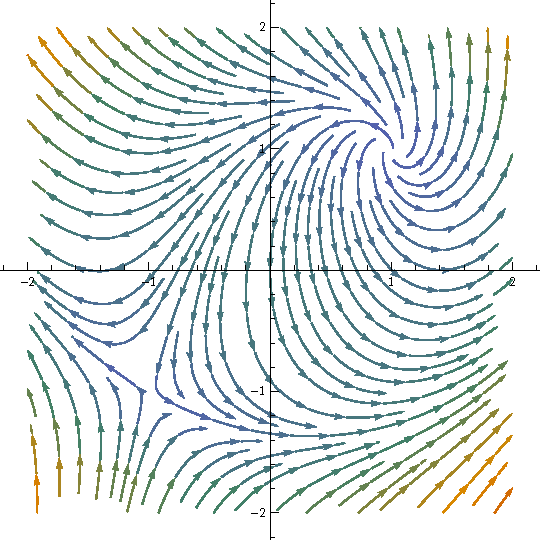
\includegraphics[width=7.5cm]{images/linearizing_system_1.pdf}\break

    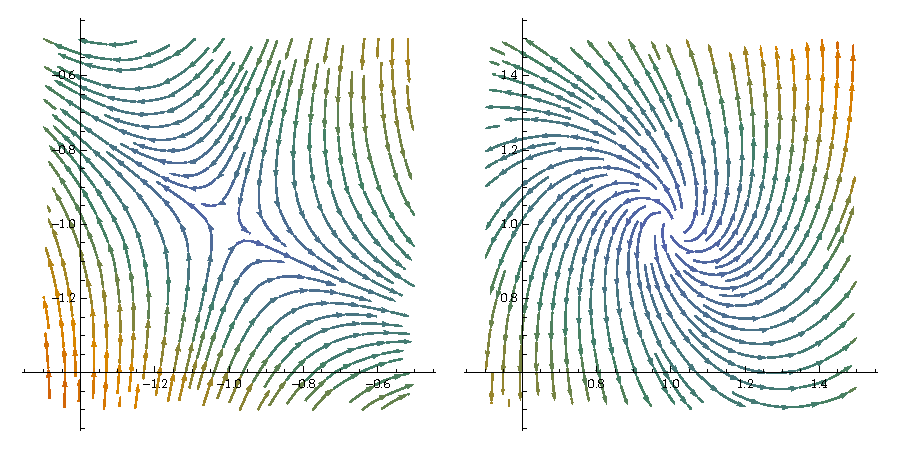
\includegraphics[width=15cm]{images/linearizing_system_1_zoomed.pdf}
  \end{center}
\end{example}
Unfortunately, there are places where linearization may fail.
\begin{example}[Linearization's Failure]
  Consider the linearization
  \begin{align*}
    \diff{x}{t} &= y - \left(x^2 + y^2\right)x\\
    \diff{y}{t} &= -x-\left(x^2 + y^2\right)y.
  \end{align*}
  Note that $\left(0,0\right)$ is an equilibrium solution. Solving the Jacobian, we find
  \begin{align*}
    J|_{\left(x,y\right)} &= \begin{pmatrix}-3x^2 - y^2 & 1-2yx\\-1-2xy & -3y^2 - x^2\end{pmatrix}
  \end{align*}
  Evaluating at the equilibrium solution, we find
  \begin{align*}
    \diff{\vec{U}}{t} &=  \begin{pmatrix}0 & 1 \\ -1 & 0\end{pmatrix} \begin{pmatrix}u\\v\end{pmatrix}.
  \end{align*}
  The eigenvalues are $\lambda = \pm i$. Thus, we find that the origin is a center. Presumably.
  \begin{center}
    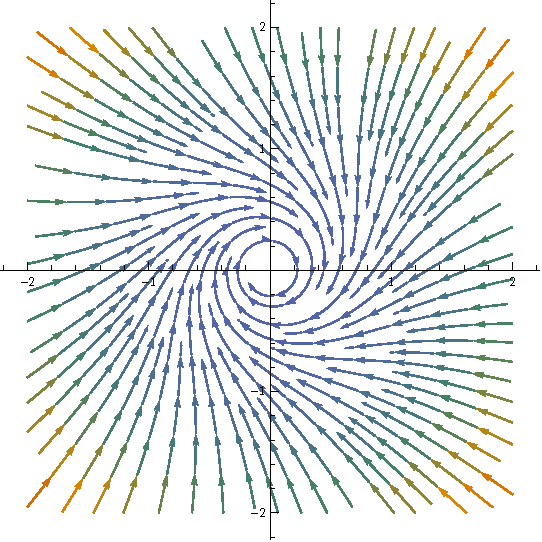
\includegraphics[width=10cm]{images/linearizing_system_2.pdf}
  \end{center}
  However, we see that solutions spiral towards the origin (very slowly).
\end{example}
Thus, we are forced to see that we cannot rely on the linearization method to solve borderline cases.\newline

In particular, the borderline cases on the trace-determinant plane occur at the points where
\begin{itemize}
  \item $T = 0$ (i.e., centers);
  \item $D = \frac{1}{4}T^2$ (i.e., repeated eigenvalues);
  \item $D = 0$ (i.e., attracting/repelling fixed points).
\end{itemize}
\end{document}
